\chapter{Surface-Wave JWKB Theory}

In this final chapter we analyze the propagation of Rayleigh
and Love waves on a non-rotating, hydrostatic,
laterally heterogeneous Earth, using a
surface-wave analogue of the body-wave JWKB theory developed
in Chapter~15.  The resulting surface-wave JWKB theory is
valid for arbitrarily large three-dimensional variations in the elastic and
anelastic properties of the Earth; however, the variations are
required to be {\em laterally smooth\/} in the sense
\index{perturbation!smooth}%
$\lambda/\Lambda_{\Omega}\ll 1$,
where $\lambda=2\pi k^{-1}$ is the
wavelength of the surface wave on the
unit sphere $\Omega$, and $\Lambda_{\Omega}$
is the corresponding angular scale
of the heterogeneity.  Smooth topographic variations on the
outer free surface and internal solid-solid and
fluid-solid discontinuities are accounted for,
as well as slowly varying lateral volumetric
heterogeneity within the aspherical sub-regions of the Earth.
As in our study of high-frequency
body waves, we base our analysis upon a {\em slowly varying
variational principle\/}, which yields local radial Love and
Rayleigh eigenfunctions, local dispersion relations, and transport
equations describing the conservation of surface-wave energy.
The dispersion relations determine the geometry
of surface-wave rays on $\Omega$,
whereas the transport equations determine
the associated Love and Rayleigh amplitude variations.

\enlargethispage{-0.5\baselineskip}

The two-dimensional character of
the propagation makes surface-wave ray
theory simpler in many respects than body-wave ray theory.
In addition, we presume there are no lateral boundaries, so
that discontinuities in geometrical spreading and coupling
between different dispersion branches need not be considered.
On the other hand, there are some additional complications;
in particular, the propagation is multi-modal and dispersive,
and rays must be traced on the curved surface of the
unit sphere rather than through three-dimensional Euclidean space.
Important contributions to surface-wave JWKB theory have been made
by Woodhouse (\citeyear{woodhouse74}), Babich, Chikhachev
\& Yanovskaya (\citeyear{babich&al76}), Yomogida
(\citeyear{yomogida85}), Yomogida \& Aki (\citeyear{yomogida&aki85}),
Woodhouse \& Wong (\citeyear{woodhouse&wong86}),
Jobert \& Jobert (\citeyear{jobert&jobert87})
and Keilis-Borok, Levshin \& others (\citeyear{keilis-borok89}).
We follow the treatment by
Tromp \& Dahlen (\citeyear{tromp&dahlen92a};
\citeyear{tromp&dahlen92b})
and Wang \& Dahlen (\citeyear{wang&dahlen94};
\citeyear{wang&dahlen95}),
adhering to our usual convention that
$\exp(-i\omega t)$ appears in the Fourier
integral upon transforming from time
$t$ to angular frequency $\omega$.

\section{Preliminaries}

As in the last chapter, we employ our customary set-theoretical
notation to describe a piecewise continuous Earth model
$\earth=\earth_{\rm S}\cup\earth_{\rm F}$ composed of
concentric solid and fluid regions separated by non-intersecting
interfaces $\Sigma=\p\earth\cup\Sigma_{\rm SS}\cup\Sigma_{\rm FS}$
with unit outward normal $\bnh$ (see Figure~3.1).  The geographically
variable radii of the outer free surface and interior solid-solid
and fluid-solid discontinuities will be denoted by
$d=a\cup d_{\rm SS}\cup d_{\rm FS}$ (see Section~8.2).
Since we seek a theory that is applicable to mantle as well as
crustal surface waves, we retain the effects of self-gravitation
in the analysis.  The displacement $\bs$ and incremental
Eulerian gravitational potential $\phi$ are governed by the
linearized momentum equation~(\ref{4.nrhydromom}) and Poisson's
equation~(\ref{3.Poisson}):
\index{equations of motion!hydrostatic}%
\eq
\label{16.eqmot}
-\omega^2\rho\hspace{0.3 mm}\bs
+\bdel(\rho\hspace{0.3 mm}\bs\cdot\bdel\phi)
+\rho\bdel\phi-[\bdel\cdot(\rho\hspace{0.3 mm}\bs)]
\bdel\phi=\bdel\cdot\bT,
\en
\eq \label{16.Poisson}
\del^2\phi=-\bdel\cdot(\rho\hspace{0.3 mm}\bs).
\en
We restrict attention to an Earth having an isotropic
elastic stress-strain relation, as in~(\ref{15.Hooke}):
\index{Hooke's law}%
\eq \label{16.Hooke}
\bT=\kappa(\bdel\cdot\bs)\bI+2\mu\bd,
\en
where $\kappa$ and $\mu$ are the isentropic incompressibility and
the rigidity, respectively, and $\bd=\half[\bdel\bs+(\bdel\bs)^{\rm T}]
-\third(\bdel\cdot\bs)\bI$ is the strain deviator.
The system of elastic-gravitational
equations~(\ref{16.eqmot})--(\ref{16.Hooke})
must be solved subject to the kinematic continuity conditions
\index{boundary conditions!kinematic}%
\index{boundary conditions!dynamic}%
\index{boundary conditions!gravitational}%
$[\bs]^+_-=\bzero$ on $\Sigma_{\rm SS}$,
$[\bnh\cdot\bs]^+_-=0$ on $\Sigma_{\rm FS}$
and $[\phi]^+_-=0$ on $\Sigma$, together with
the dynamical and gravitational boundary
conditions~(\ref{4.hydrobc1})--(\ref{4.hydrobc3})
and~(\ref{3.surfmass}):
\eq \label{16.bceqn1}
\bnh\cdot\bT=\bzero\quad\mbox{on $\p\earth$},
\en
\eq \label{16.bceqn2}
[\bnh\cdot\bT]^+_-=\bzero\quad\mbox{on $\Sigma_{\rm SS}$},
\en
\eq \label{16.bceqn3}
[\bnh\cdot\bT]^+_-=\bnh[\bnh\cdot\bT\cdot\bnh]^+_-
=\bzero\quad\mbox{on $\Sigma_{\rm FS}$},
\en
\eq \label{16.bceqn4}
[\bnh\cdot\bdel\phi+4\pi G\rho\bnh\cdot\bs]^+_-=0
\quad\mbox{on all of $\Sigma$.}
\en
Since we are interested in the propagation
of transient waves, it is essential to regard
$\bs(\bx,\om)$, $\phi(\bx,\om)$ and $\bT(\bx,\om)$ as
{\em complex\/}.  As in Chapter~15, we consider
the real angular frequency to be positive: $\om>0$.

The equations of motion~(\ref{16.eqmot})--(\ref{16.Poisson})
and associated boundary conditions~(\ref{16.bceqn1})--(\ref{16.bceqn4})
can be obtained from the variational principle $\delta\sI'=0$,
where
\index{variational principle!surface-wave}%
\index{surface-wave variational principle}%
\index{action!surface-wave}%
\index{surface-wave action}%
\eq \label{16.I'}
\sI'=\int_{\subspace} L'(\bs,\bdel\bs,\bdel\phi\,;\,
\bs^*,\bdel\bs^*,\bdel\phi^*)\,dV.
\en
The integration in equation~(\ref{16.I'}) is over all of
space $\allspace$; the integrand is the
Lagrangian density in an isotropic Earth, given by
\index{Lagrangian density!surface-wave}%
\index{surface-wave Lagrangian density}%
\eqa \label{16.L'}
\lefteqn{
L'=\half[\om^2\rho\hspace{0.3 mm}\bs^*\cdot\bs
-\kappa(\bdel\cdot\bs^*)(\bdel\cdot\bs)
-2\mu\bd^*\!:\!\bd
} \nonumber \\
&&\mbox{}
-\rho(\bs^*\cdot\bdel\phi+\bs\cdot\bdel\phi^*)
-\rho\hspace{0.3 mm}\bs^*\cdot\bdel\bdel\Phi\cdot\bs
\nonumber \\
&&\mbox{}
-\half\rho\bdel\Phi\cdot(\bs^*\cdot\bdel\bs+\bs\cdot\bdel\bs^*
-\bs^*\bdel\cdot\bs-\bs\bdel\cdot\bs^*)
\nonumber \\
&&\mbox{}
-(4\pi G)^{-1}\bdel\phi^*\cdot\bdel\phi],
\ena
where $\Phi$ is the initial gravitational potential and $G$
is the gravitational constant.  Equations~(\ref{16.I'})
and~(\ref{16.L'}) are the travelling-wave equivalents of
the standing-wave action~(\ref{4.hydroact2}) and Lagrangian
density~(\ref{4.ZOOT}).  It is convenient to regard $\bs$ and
$\phi$ as independent variables in the present application;
for that reason, we base our JWKB analysis upon the
{\em modified\/} action $\sI'$ and Lagrangian density
\index{modified action}%
\index{action!modified}%
$L'$ rather than the travelling-wave versions
of~(\ref{4.hydroact}) and~(\ref{4.ZOOTME}).
The variation of the modified action~(\ref{16.I'}) is
\eqa \label{16.varact} \lefteqn{
\delta\sI'=2\,\Re{\rm e}\int_{\subearth}\bdelta\bs^*\cdot
\left[\p_{\subs^*}L'-\bdel\cdot(\p_{\sbdel\subs^*}L')\right] dV} \nonumber \\
&&\mbox{}-2\,\Re{\rm e}\int_{\subspace}\delta\phi^*\,
[\bdel\cdot(\p_{\sbdel\phi^*}L')]\,dV \nonumber \\
&&\mbox{}-2\,\Re{\rm e}\int_{\Sigma}\left[\bdelta\bs^*\cdot
(\bnh\cdot\p_{\sbdel\subs^*}L')+\bdelta\phi^*
(\bnh\cdot\p_{\sbdel\phi^*}L')\right]^+_-\,d\/\Sigma.
\ena
This vanishes for arbitrary independent variations
$\bdelta\bs$ and $\delta\phi$ satisfying the admissibility
constraints $[\bdelta\bs]^+_-=\bzero$ on $\Sigma_{\rm SS}$,
$[\bnh\cdot\bdelta\bs]^+_-=0$ on $\Sigma_{\rm FS}$
and $[\delta\phi]^+_-=0$ on $\Sigma$ if and only if
$\bs$ and $\phi$ satisfy the Euler-Lagrange equations
\index{Euler-Lagrange equations!surface-wave}%
\eq \label{16.ELeqn1}
\p_{\subs^*}L'-\bdel\cdot(\p_{\sbdel\subs^*}L')\quad\mbox{in $\earth$},
\en
\eq \label{16.ELeqn2}
\bdel\cdot(\p_{\sbdel\phi^*}L')\quad\mbox{in $\allspace$}
\en
and associated boundary conditions
\eq \label{16.ELbc1}
\bnh\cdot(\p_{\sbdel\subs^*}L')=\bzero\quad\mbox{on $\p\earth$},
\en
\eq \label{16.ELbc2}
[\bnh\cdot(\p_{\sbdel\subs^*}L')]^+_-=\bzero\quad\mbox{on $\Sigma_{\rm SS}$},
\en
\eq \label{16.ELbc3}
[\bnh\cdot(\p_{\sbdel\subs^*}L)]^+_-=
\bnh[\bnh\cdot(\p_{\sbdel\subs^*}L)\cdot\bnh]^+_-
=\bzero\quad\mbox{on $\Sigma_{\rm FS}$},
\en
\eq \label{16.ELbc4}
[\bnh\cdot(\p_{\sbdel\phi^*}L')]^+_-=0\quad\mbox{on $\Sigma$}.
\en
Equations~(\ref{16.ELeqn1})--(\ref{16.ELeqn2})
and~(\ref{16.ELbc1})--(\ref{16.ELbc4}) are identical
to~(\ref{16.eqmot})--(\ref{16.Poisson})
and~(\ref{16.bceqn1})--(\ref{16.bceqn4}).
The value of the modified action at the stationary
transient solution is $\sI'=0$.

The volumetric energy density associated with
the Lagrangian density~(\ref{16.L'}) is
\index{energy density!surface-wave}%
\index{surface-wave energy density}%
$E=E'=\om\p_{\omega}L'-L'$.  A more useful quantity in the present
instance is the radially integrated {\em surface energy density\/},
defined by
\eq \label{16.E_Om}
E_\Omega=\int_0^\infty(\om\p_{\omega}L'-L')\,r^2dr.
\en
The transient, frequency-domain analogue of the elastic-gravitational
energy flux~(\ref{3.K'in16}) is
\index{energy flux!surface-wave}%
\index{surface-wave energy flux}%
\eqa \label{16.K'} \lefteqn{
\bK'=\Re{\rm e}\,\{i\om[\kappa\hspace{0.2 mm}\bs^*(\bdel\cdot\bs)
+2\mu(\bs^*\cdot\bd)}
\nonumber \\
&&\mbox{}\qquad\qquad-\rho\hspace{0.2 mm}\bs^*(\bs\cdot\bdel\Phi)
+\rho\hspace{0.2 mm}\phi^*\bs+(4\pi G)^{-1}\phi^*\bdel\phi]\}.
\ena
In this case, the interesting quantity is the {\em total lateral
flux of energy\/}:
\index{energy flux!surface-wave}%
\index{surface-wave energy flux}%
\eq \label{16.K'_Om}
\bK_{\Omega}^{\prime}=\int_0^{\infty}(\bI-\brh\brh)
\cdot\bK'\,r\hspace{0.2 mm}dr.
\en
The surface through which the energy passes is a
cone extending outward from the center of the Earth;
the differential $r\hspace{0.2 mm}dr$ accounts for the
radial dependence of the area of a patch on this cone.
Both $E_{\Omega}$ and $\bK_{\Omega}^{\prime}$ may
be regarded as functions of position $\brh$ on the unit
sphere $\Omega$.  Written out explicitly, these surficial
variables are
\eqa \label{16.E_Om2} \lefteqn{
E_\Omega=\half\int_0^{\infty}[\om^2\rho\hspace{0.3 mm}\bs^*\cdot\bs
+\kappa(\bdel\cdot\bs^*)(\bdel\cdot\bs)
+2\mu\bd^*\!:\!\bd} \nonumber \\
&&\mbox{}
+\rho(\bs^*\cdot\bdel\phi+\bs\cdot\bdel\phi^*)
+\rho\hspace{0.3 mm}\bs^*\cdot\bdel\bdel\Phi\cdot\bs
\nonumber \\
&&\mbox{}
+\half\rho\bdel\Phi\cdot(\bs^*\cdot\bdel\bs+\bs\cdot\bdel\bs^*
+\bs^*\bdel\cdot\bs-\bs\bdel\cdot\bs^*)
\nonumber \\
&&\mbox{}
+(4\pi G)^{-1}\bdel\phi^*\cdot\bdel\phi]\,r^2dr,
\ena
\eqa \label{16.K'_Om2} \lefteqn{
\bK_{\Omega}^{\prime}=\Re{\rm e}
\int_0^{\infty}i\om(\bI-\brh\brh)\cdot
[\kappa\hspace{0.2 mm}\bs^*(\bdel\cdot\bs)
+2\mu(\bs^*\cdot\bd)}
\nonumber \\
&&\mbox{}\qquad-\rho\hspace{0.2 mm}\bs^*(\bs\cdot\bdel\Phi)
+\rho\hspace{0.2 mm}\phi^*\bs+(4\pi G)^{-1}\phi^*\bdel\phi]\,r\hspace{0.2 mm}dr.
\ena
The integration extends outward to infinity in
both~(\ref{16.E_Om2}) and~(\ref{16.K'_Om2});
however, only the gravitational-field self-energy
$(8\pi G)^{-1}\bdel\phi^*\cdot\bdel\phi$ and the
purely gravitational flux
${\rm Re}\,[i\omega(4\pi G)^{-1}\phi^*\bdel\phi]$
are non-zero outside of the Earth, in $\allspace-\earth$.
The units of $E_\Omega$ and $\bK_{\Omega}^{\prime}$ are
energy per steradian and energy per unit time per radian
of wavefront arc on $\Omega$, respectively.

\section{Slow Variational Principle}
\index{variational principle!slow|(}%
\index{slow variational principle!surface waves|(}%

Guided by the vector representation~(\ref{B.sphtor}),
we seek JWKB solutions to
\index{JWKB solution!surface waves}%
equations~(\ref{16.eqmot})--(\ref{16.Poisson})
and~(\ref{16.bceqn1})--(\ref{16.bceqn4}) of the form
\eqa \label{16.JWKB} \lefteqn{
\bs=(U\brh+k_{\rm R}^{-1}V\bdel_1)A_{\rm R}\exp(-i\psi_{\rm R})}
\nonumber \\
&&\mbox{}\qquad
-k_{\rm L}^{-1}W(\brh\times\bdel_1)A_{\rm L}\exp(-i\psi_{\rm L}),
\ena
\eqa \label{16.JWKB_phi} \lefteqn{
\phi=PA_{\rm R}\exp(-i\psi_{\rm R}),}
\ena
where the subscripts R and L stand for {\em Rayleigh\/} and
{\em Love\/}, respectively.  The amplitudes $A_{\rm R}$,
$A_{\rm L}$ and phases $\psi_{\rm R}$, $\psi_{\rm L}$ are
\index{amplitude!Love-wave}%
\index{amplitude!Rayleigh-wave}%
\index{surface-wave amplitude}%
\index{phase!Love-wave}%
\index{phase!Rayleigh-wave}%
\index{surface-wave phase}%
presumed to be real.
On a spherically symmetric Earth the radial eigenfunctions
$U$, $V$, $W$ and $P$ are functions of radius~$r$ only,
and the complex quantities
$A_{\rm R}\exp(-i\psi_{\rm R})$ and
$A_{\rm L}\exp(-i\psi_{\rm L})$ are
travelling-wave Legendre functions of the form
\eq
A\exp(-i\psi)\sim Q_{k-\subhalf\,m}^{(1,2)}(\cos\theta)\exp(im\phi),
\en
as discussed in Chapter~11.
On a laterally heterogeneous Earth,
the real functions $U$, $V$, $W$ and $P$ are
regarded as {\em local radial eigenfunctions\/},
\index{local radial eigenfunction}%
\index{radial eigenfunction!local}%
which depend not only upon the radius $r$ but also upon
the geographical position $\brh=(\theta,\phi)$ on the unit sphere.
The real {\em local Rayleigh and Love wavevectors\/} are
\index{wavevector}%
\index{local wavevector}%
defined in terms of the phases $\psi_{\rm R}$ and $\psi_{\rm L}$ by
\eq \label{16.wavevectors}
\bk_{\rm R}=\bdel_1\psi_{\rm R},
\qquad
\bk_{\rm L}=\bdel_1\psi_{\rm L}.
\en
The associated scalar local wavenumbers
\index{local wavenumber}%
\index{wavenumber!local}%
are $k_{\rm R}=||\bk_{\rm R}||$ and $k_{\rm L}=||\bk_{\rm L}||$.

As in Section~\ref{15.sec.slow}, we obtain a {\em slowly varying action\/}
by substituting the JWKB representation~(\ref{16.JWKB})--(\ref{16.JWKB_phi})
into~(\ref{16.I'}) and retaining only the lowest-order terms in the
small parameter $\lambda/\hspace{-0.3 mm}\Lambda_{\Omega}$.
The resulting JWKB action separates naturally into
distinct Rayleigh- and Love-wave parts:
\index{action!slow}%
\index{slow action!surface waves}%
\eq \label{16.actsum}
\sI'=\sI'_{\rm R}+\sI_{\rm L},
\en
where
\eq
\label{16.Ract}
\sI'_{\rm R}=\int_{\subspace}\sL'_{\rm R}(U,V,P,\p_rU,\p_rV,\p_rP,
A_{\rm R},\bdel_1\psi_{\rm R})\,dV,
\en
\eq
\label{16.Lact}
\sI_{\rm L}=\int_{\subearth}\sL_{\rm L}
(W,\p_rW,A_{\rm L},\bdel_1\psi_{\rm L})\,dV.
\en
We have retained the primes upon $\sI'_{\rm R}$
and $\sL'_{\rm R}$, but dropped them upon $\sI_{\rm L}$ and $\sL_{\rm L}$,
since Love waves are unaccompanied by any gravitational perturbation.
The integrands in~(\ref{16.Ract}) and~(\ref{16.Lact}) are
{\em slowly varying Lagrangian densities\/} analogous to~(\ref{15.sLden}):
\index{Lagrangian density!slow}%
\index{slow Lagrangian density!surface waves}%
\eqa \label{16.sL'_R}
\lefteqn{
\sL_{\rm R}^{\prime}=\half[\om^{2\!}\rho(U^2+V^2)
-\kappa(\p_rU+2r^{-1}U-kr^{-1}V)^2} \nonumber \\
&&\mbox{}-\third\mu(2\p_rU-2r^{-1}U+kr^{-1}V)^2
-\mu(\p_rV-r^{-1}V-kr^{-1}U)^2 \nonumber \\
&&\mbox{}\qquad-(k^2-2)\mu r^{-2}V^2
-2\rho(U\p_rP+kr^{-1}VP) \nonumber \\
&&\mbox{}\qquad\qquad-4\pi G\rho^2U^2
+2\rho gr^{-1}U(2U-kV) \nonumber \\
&&\mbox{}\qquad\qquad\qquad
-(4\pi G)^{-1}(\p_rP^2+k^2r^{-2}P^2)]\hspace{0.3 mm}A_{\rm R}^2,
\ena
\eq \label{16.sL'_L}
\sL_{\rm L}=\half[\om^{2\!}\rho W^2
-\mu(\p_rW-r^{-1}W)^2
-(k^2-2)\mu r^{-2}W^2]
\hspace{0.3 mm}A_{\rm L}^2.
\en
As in our discussion of body waves, we shall
use script letters throughout this chapter to denote
densities and other quantities that vary on the slow
scale $\Lambda_{\Omega}$ of the lateral heterogeneity; the wavelength-scale
variations associated with the exponentials $\exp(-i\psi_{\rm R})$
and $\exp(-i\psi_{\rm L})$ have been eliminated in~(\ref{16.sL'_R})
and~(\ref{16.sL'_L}).  The Rayleigh-wave density $\sL'_{\rm R}$ depends upon
$U,V,P,\p_rU,\p_rV,\p_rP,A_{\rm R}$ and the wavevector $\bdel_1\psi_{\rm R}$,
whereas the Love-wave density $\sL_{\rm L}$ depends upon
$W,\p_rW,A_{\rm L}$ and $\bdel_1\psi_{\rm L}$, as indicated
by the arguments in equations~(\ref{16.Ract})--(\ref{16.Lact}).
We have dropped the subscript R upon
$k_{\rm R}=\|\bdel_1\psi_{\rm R}\|$ in~(\ref{16.sL'_R})
and the subscript L upon
$k_{\rm L}=\|\bdel_1\psi_{\rm L}\|$ in~(\ref{16.sL'_L}) to
facilitate the comparison of $\sL'_{\rm R}$ and
$\sL_{\rm L}$ with the corresponding one-dimensional
Lagrangian densities~(\ref{eq:8.spherl2})
and~(\ref{eq:8.torl}).  Apart from the
three-dimensionality and the extra
amplitude factors $A_{\rm R}^2$ and $A_{\rm L}^2$,
the only difference is the replacement of the
ordinary radial derivatives $\dot{U}$, $\dot{V}$, $\dot{W}$
and $\dot{P}$ by the partial derivatives $\p_rU$,
$\p_rV$, $\p_rW$ and $\p_rP$.

The decomposition~(\ref{16.actsum}) of the slowly
varying action $\sI'$ into separate terms $\sI'_{\rm R}$ and
$\sI_{\raisebox{-0.2 ex}{\scriptsize\rm L}}$ is an indication
that Rayleigh and Love waves propagate independently,
to lowest order in the small parameter
$\lambda/\hspace{-0.3 mm}\Lambda_{\Omega}$.
Fundamental and overtone waves of the same type are likewise
uncoupled; a surface wave of a given type and overtone number
{\em clings to its identity\/} as it propagates.
All of the information needed to trace surface-wave rays and
connect the amplitudes $A_{\rm R}$, $A_{\rm L}$, the phases
$\psi_{\rm R}$, $\psi_{\rm L}$ and the wavevectors
$\bk_{\rm R}$, $\bk_{\rm L}$ at points along
those rays is contained in the slowly varying Rayleigh
and Love Lagrangian densities $\sL'_{\rm R}$ and
$\sL_{\raisebox{-0.2 ex}{\scriptsize\rm L}}$.
We consider the two types of surface waves separately in the
next two sections, treating the easier case first.

\subsection{Love waves}
\index{Love wave|(}%}%
\index{surface wave!Love|(}%}%

Dropping the subscripts upon $\sI_{\rm L}$, $\sL_{\rm L}$
and $A_{\rm L}$ for the sake of brevity,
we consider the {\em slow Love-wave variational principle\/}
\index{slow variational principle!Love waves}%
\eqa \label{16.deltaI_L} \lefteqn{
\delta\sI=\int_{\subearth}\delta W\hspace{-0.3 mm}
\left[\p_W\sL-r^{-2}\p_r
(r^2\p_{\partial_r\hspace{-0.3 mm}W}\sL)\right]dV} \nonumber \\
&&\mbox{}+\sum_d\left[\delta W\hspace{0.3 mm}
(\p_{\partial_r\hspace{-0.3 mm}W}\sL)\right]^+_- \nonumber \\
&&\mbox{}+\int_{\Omega}\delta A\left[\int_0^a
(\p_A\sL)\,r^2dr\right]d\/\Omega \nonumber \\
&&\mbox{}
+\int_{\Omega}\delta\psi\left\{\bdel_1\cdot
\left[\int_0^a(\p_{\sbdel_{\hspace{-0.3 mm}1}\psi}\sL)\,r^2dr\right]
\right\}d\/\Omega=0.
\ena
The second and third integrals involving the
variations $\delta A$ and $\delta\psi$ are
over the unit sphere $\Omega$, because the
amplitude $A$ and phase $\psi$ are independent
of the radius $r$.  The variation~(\ref{16.deltaI_L})
vanishes for arbitrary variations satisfying the admissibility
constraint $[\delta W]^+_-=0$ on $r=d_{\rm SS}$
if and only if the fields $W$, $A$ and $\psi$
satisfy the three Euler-Lagrange equations
\index{Euler-Lagrange equations!Love-wave}%
\eq \label{16.elL1}
\p_W\sL-r^{-2}\p_r(r^2\p_{\partial_r\hspace{-0.3 mm}W}\sL)=0
\quad\mbox{in $0\leq r\leq a$},
\en
\eq \label{16.elL2}
\int_0^a(\p_A\sL)\,r^2dr=0\quad\mbox{on $\Omega$},
\en
\eq \label{16.elL3}
\bdel_1\cdot\left[\int_0^a(\p_{\sbdel_{\hspace{-0.3 mm}1}\psi}\sL)\,r^2dr\right]=0
\quad\mbox{on $\Omega$},
\en
together with the boundary conditions
\eq \label{16.bcL1}
\p_{\partial_r\hspace{-0.3 mm}W}\sL=0\quad\mbox{on $r=a$ and $r=d_{\rm FS}$},
\en
\eq \label{16.bcL2}
[\p_{\partial_r\hspace{-0.3 mm}W}\sL]_-^+=0\quad\mbox{on $r=d_{\rm SS}$}.
\en
Written out explicitly, equation~(\ref{16.elL1}) is
\eqa \label{16.W}
\lefteqn{r^{-2}\p_r[\mu r^2(\p_rW-r^{-1}W)]
+\mu r^{-1}(\p_rW-r^{-1}W)} \nonumber \\
&&\mbox{}+[\om^{2\!}\rho-(\sqL^2-2)\mu r^{-2}]W=0.
\ena
The quantity $-\p_{\partial_r\hspace{-0.3 mm}W}\sL$
is precisely the local traction $T=\mu(\p_rW-r^{-1}W)$, so the
local boundary conditions~(\ref{16.bcL1})--(\ref{16.bcL2}) are
\eq \label{16.T1}
T=0\quad\mbox{on $r=a$ and $r=d_{\rm FS}$},
\en
\eq \label{16.T2}
[T]_-^+=0\quad\mbox{on $r=d_{\rm SS}$}.
\en
Equations~(\ref{16.W}) and~(\ref{16.T1})--(\ref{16.T2}) are identical to the
relations~(\ref{eq:8.W}) and~(\ref{8.bcneed})--(\ref{eq:8.dfsT})
that determine the Love-wave displacement $W$ and traction $T$
on a spherically symmetric Earth; the only difference is that
differentiation $d/\hspace{-0.3 mm}dr$ is replaced by partial
differentiation $\p_r$.  Recall that the free surface and interior
discontinuity surfaces
$d=a\cup d_{\rm SS}\cup d_{\rm FS}$ may exhibit slowly varying
topographic variations.

The above results should be interpreted in the following manner.
At every geographical position $\brh=(\theta,\phi)$ in a laterally
heterogeneous Earth, we construct a hypothetical spherically
symmetric model having the same structure $\kappa$,
$\mu$, $\rho$, $d$ as that underlying the surface point $a\brh$.
By repeatedly solving equations~(\ref{16.W})
and~(\ref{16.T1})--(\ref{16.T2}), we can determine
the {\em local radial eigenfunction\/}~$W$ and the associated
\index{local radial eigenfunction}%
\index{radial eigenfunction!local}%
\index{local wavenumber}%
\index{wavenumber!local}%
{\em local wavenumber\/}~$k$ at every point $\brh$
and every angular frequency $\om$.  In normal-mode calculations
we fix the angular degree $l$ and therefore the wavenumber
$k=\sqrt{l(l+1)}$, and we determine the fundamental and
higher-overtone eigenfrequencies $\om$; in surface-wave
calculations, it is preferable to fix $\om$ and determine
the wavenumbers $k$.  We think of a monochromatic Love
wave as propagating from point to point on the surface of
the unit sphere $\Omega$.
As a wave propagates, it ``carries'' its local radial structure
$W$ and wavenumber $k$ with it.  In the language of classical
mechanics, we say that $W$ and $k$ vary {\em adiabatically\/}
\index{adiabatic variation}%
along the surface-wave ray.

The second slow Euler-Lagrange equation (\ref{16.elL2}) is the
slowly varying analogue of the {\em Love-wave dispersion
relation\/}~(\ref{11.tordisp}):
\index{dispersion!Love-wave}%
\index{Love-wave dispersion}%
\eq \label{16.locdisL}
\om^2I_1-k^2I_2-I_3=0.
\en
The local radial integrals $I_1$, $I_2$ and $I_3$ are identical
to~(\ref{11.Lint1})--(\ref{11.Lint3}), with $\dot{W}$ replaced
by $\p_rW$:
\eq \label{16.I1L}
I_1=\int_0^a\rho W^2\,r^2dr,
\en
\eq \label{16.I2L}
I_2=\int_0^a\mu W^2\,dr,
\en
\eq \label{16.I3L}
I_3=\int_0^a\mu[(\p_rW-r^{-1}W)^2-2r^{-2}W^2]\,r^2dr.
\en
By subtracting the local dispersion relations for two
waves with associated frequencies $\om$ and $\om+\delta\om$,
local wavenumbers $k$ and $k+\delta\hspace{-0.1 mm}k$,
and local radial eigenfunctions $W$ and $W+\delta W$,
we find that the
{\em local group speed\/} $C=d\om\hspace{-0.3 mm}
\index{local group speed}%
\index{group speed!local}%
\index{local phase speed}%
\index{phase speed!local}%
/\hspace{-0.3 mm}d\hspace{-0.1 mm}k$ and {\em phase speed\/}
$c=\om/k$ of a Love wave are related by the slowly
varying analogue of~(\ref{11.Lgrvel}):
\eq \label{16.Lgrvel}
C=\frac{I_2}{cI_1}.
\en
Both $C$ and $c$ are {\em angular\/} rates of propagation,
measured in radians per second on the surface
of the unit sphere $\Omega$.
We shall use the local dispersion relation~(\ref{16.locdisL}) as the basis
for kinematic Love-wave ray tracing in Section~\ref{16.sec.raytrace}.
In this sense, it is analogous to the eikonal equation~(\ref{15.geikonal})
for body waves.

The slowly varying energy density and lateral energy flux
obtained by substituting the JWKB representation
$\bs=-k^{-1}W(\brh\times\bdel_1)A\exp(-i\psi)$ into
equations~(\ref{16.E_Om2}) and~(\ref{16.K'_Om2}) are
\index{energy density!slow}%
\index{energy flux!slow}%
\index{slow energy density!Love waves}%
\index{slow energy flux!Love waves}%
\eq \label{16.sE_OmL}
\sE_\Omega=\half(\om^2I_1+k^2I_2+I_3)A^2=\om^2I_1A^2,
\en
\eq \label{16.KOmL}
\bsK_{\Omega}=\om I_2A^2\bk=C\sE_{\Omega}\bkh.
\en
We have dropped the prime upon $\bsK_{\Omega}=\bsK_{\Omega{\rm L}}$,
and used the dispersion relation~(\ref{16.locdisL})
and the group-speed identity~(\ref{16.Lgrvel}) to obtain the
final results in~(\ref{16.sE_OmL}) and~(\ref{16.KOmL}),
respectively.  The energy density~(\ref{16.sE_OmL}) is
the sum of the kinetic energy density $\half\om^2I_1A^2$
and the elastic potential energy density $\half(k^2I_2+I_3)A^2$.
The dispersion relation stipulates
that the energy of a propagating Love wave is equipartitioned; the total
surface energy density is therefore twice the kinetic energy
density.  The magnitude of the Love-wave energy flux
$\|\bsK_{\Omega}\|$ is the product of the wave
speed $C$ and the energy density $\sE_{\Omega}$, as
in the case of body waves.  It is noteworthy that it
is $C$ rather than the phase speed $c$ that appears
in equation~(\ref{16.KOmL}); this is because the
{\em energy of a dispersive wave propagates with
the group speed\/}.

The final Euler-Lagrange equation~(\ref{16.elL3}) is the Love-wave
analogue of the {\em transport equation\/}~(\ref{15.transport}):
\index{transport equation!Love waves}%
\eq \label{16.transL}
\bdel_1\cdot\bsK_{\Omega}=0.
\en
This equation determines the variation in Love-wave amplitude
along a ray, as we shall see in Section~\ref{16.sec.amplitudes}.
The local dispersion relation (\ref{16.locdisL})
and the transport equation (\ref{16.transL}) can also
be obtained from the {\em surface variational principle\/}
\index{variational principle!surface}%
$\delta\sI_\Omega=0$, where
\eq \label{16.sI_OmL}
\sI_\Omega=\int_\Omega\sL_\Omega(A,\bdel_1\psi)\,d\Omega.
\en
The {\em slowly varying surface Lagrangian density\/}
in~(\ref{16.sI_OmL}) is given by
\eq \label{16.L_OmL}
\sL_\Omega=\int_0^a\sL\,r^2dr=\half(\om^2I_1-k^2I_2-I_3)A^2.
\en
The surface Lagrangian and energy densities are related
to each other by a Legendre transformation, as usual:
$\sE_{\Omega}=\om\p_{\omega}\sL_{\Omega}-\sL_{\Omega}$.
The flux~(\ref{16.KOmL}) can be written in the form
$\bsK_{\Omega}=\p_{\subk}\sL_{\Omega}$.
\index{Love wave|)}%}%
\index{surface wave!Love|)}%}%

\subsection{Rayleigh waves}
\index{Rayleigh wave|(}%}%
\index{surface wave!Rayleigh|(}%}%

The variation of the slowly varying Rayleigh-wave
action~(\ref{16.Ract}) can be written in a manner
analogous to~(\ref{16.deltaI_R}):
\index{slow variational principle!Rayleigh waves}%
\eqa \label{16.deltaI_R} \lefteqn{
\delta\sI'=\int_{\subearth}\delta U\hspace{-0.3 mm}
\left[\p_U\sL'-r^{-2}\p_r
(r^2\p_{\partial_r\hspace{-0.1 mm}U}\sL')\right]dV} \nonumber \\
&&\mbox{}+\int_{\subearth}\delta V\hspace{-0.3 mm}
\left[\p_V\sL'-r^{-2}\p_r
(r^2\p_{\partial_r\hspace{-0.3 mm}V}\sL')\right]dV \nonumber \\
&&\mbox{}+\int_{\subspace}\delta P\hspace{-0.3 mm}
\left[\p_P\sL'-r^{-2}\p_r
(r^2\p_{\partial_r\hspace{-0.1 mm}P}\sL')\right]dV \nonumber \\
&&\mbox{}+\sum_d\left[\delta U\hspace{0.3 mm}
(\p_{\partial_r\hspace{-0.1 mm}U}\sL')+\delta V\hspace{0.3 mm}
(\p_{\partial_r\hspace{-0.3 mm}V}\sL')+\delta P\hspace{0.3 mm}
(\p_{\partial_r\hspace{-0.1 mm}P}\sL')\right]^+_- \nonumber \\
&&\mbox{}+\int_{\Omega}\delta A\left[\int_0^{\infty}
(\p_A\sL')\,r^2dr\right]d\/\Omega \nonumber \\
&&\mbox{}
+\int_{\Omega}\delta\psi\left\{\bdel_1\cdot
\left[\int_0^{\infty}(\p_{\sbdel_{\hspace{-0.3 mm}1}\psi}\sL')\,r^2dr\right]
\right\}d\/\Omega=0,
\ena
where we have dropped the subscripts upon
$\sI_{\rm R}^{\prime}$ and $\sL_{\rm R}^{\prime}$ for simplicity.
This vanishes for arbitrary variations satisfying the
admissibility constraints $[\delta U]^+_-=0$ on $r=d$,
$[\delta V]^+_-=0$ on $r=d_{\rm SS}$ and $[\delta P]^+_-=0$
on $r=d$ if and only if  $U$, $V$, $P$, $A$ and $\psi$
satisfy the Euler-Lagrange equations
\index{Euler-Lagrange equations!Rayleigh-wave}%
\eq \label{16.elR1}
\p_U\sL'-r^{-2}\p_r(r^2\p_{\partial_r\hspace{-0.1 mm}U}\sL')=0
\quad\mbox{in $0\leq r\leq a$},
\en
\eq \label{16.elR2}
\p_V\sL'-r^{-2}\p_r(r^2\p_{\partial_r\hspace{-0.3 mm}V}\sL')=0
\quad\mbox{in $0\leq r\leq a$},
\en
\eq \label{16.elR3}
\p_P\sL'-r^{-2}\p_r(r^2\p_{\partial_r\hspace{-0.1 mm}P}\sL')=0
\quad\mbox{in $0\leq r\leq\infty$},
\en
\eq \label{16.elR4}
\int_0^a(\p_{A}\sL')\,r^2dr=0\quad\mbox{on $\Omega$},
\en
\eq \label{16.elR5}
\bdel_1\cdot\left[\int_0^a(\p_{\sbdel_{\hspace{-0.3 mm}1}\psi}\sL')\,r^2dr\right]=0
\quad\mbox{on $\Omega$},
\en
together with the boundary conditions
\eq \label{16.bcR1}
\p_{\partial_r\hspace{-0.1 mm}U}\sL'=\p_{\partial_r\hspace{-0.3 mm}V}\sL'=0
\quad\mbox{on $r=a$},
\en
\eq \label{16.bcR2}
[\p_{\partial_r\hspace{-0.1 mm}U}\sL']^+_-=
[\p_{\partial_r\hspace{-0.3 mm}V}\sL']^+_-=0
\quad\mbox{on $r=d_{\rm SS}$},
\en
\eq \label{16.bcR3}
[\p_{\partial_r\hspace{-0.1 mm}U}\sL']^+_-=
\p_{\partial_r\hspace{-0.3 mm}V}\sL'=0
\quad\mbox{on $r=d_{\rm FS}$},
\en
\eq \label{16.bcR4}
[\p_{\partial_r\hspace{-0.1 mm}P}\sL']^+_-=0
\quad\mbox{on $r=d$}.
\en
Written out explicitly, equations (\ref{16.elR1})--(\ref{16.elR3})
are
\eqa \label{16.U} 
\lefteqn{r^{-2}\p_r[r^2(\kappa+\fourthirds\mu)\p_rU
+(\kappa-\twothirds\mu) r(2U-\sqL V)]} \nonumber \\
&&\mbox{}+r^{-1}[(\kappa+\fourthirds\mu)\p_rU
+(\kappa-\twothirds\mu) r^{-1}(2U-\sqL V)] \nonumber \\
&&\mbox{}
-3\kappa r^{-1}(\p_rU+2r^{-1}U-\sqL r^{-1}V) \\
&&\mbox{}-\sqL\mu r^{-1}(\p_rV-r^{-1}V+\sqL r^{-1}U)+\om^{2\!}\rho U
\nonumber \\
&&\mbox{}-\rho[\p_rP
+(4\pi G\rho-4gr^{-1})U+\sqL gr^{-1}V]=0, \nonumber
\ena
\eqa \label{16.V}
\lefteqn{r^{-2}\p_r[\mu r^2(\p_rV-r^{-1}V+\sqL r^{-1}U)]}
\nonumber \\
&&\mbox{}+\mu r^{-1}(\p_rV-r^{-1}V+\sqL r^{-1}U)
\nonumber \\
&&\mbox{}+\sqL(\kappa-\twothirds\mu)r^{-1}\p_rU
+\sqL(\kappa+\third\mu)r^{-2}(2U-\sqL V) \nonumber \\
&&\mbox{}+[\om^{2\!}\rho-(\sqL^2-2)\mu r^{-2}]V
-\sqL\rho r^{-1}(P+gU)=0,
\ena
\eqa \label{16.P} \lefteqn{
\p_r^2P+2r^{-1}\p_rP-k^2r^{-2}P} \nonumber \\
&&\mbox{}=-4\pi G(\p_r\rho)U
-4\pi G\rho\hspace{0.2 mm}[\p_rU+r^{-1}(2U-\sqL V)].
\ena
The partial derivatives
$-\p_{\raisebox{0.5 ex}{$\scriptstyle\partial_r\hspace{-0.1 mm}U$}}\sL'$,
$-\p_{\raisebox{0.5 ex}{$\scriptstyle\partial_r\hspace{-0.3 mm}V$}}\sL'$ and
$-\p_{\raisebox{0.5 ex}{$\scriptstyle\partial_r\hspace{-0.1 mm}P$}}\sL$
are the tractions $R=(\kappa+\fourthirds\mu)\p_rU
+(\kappa-\twothirds\mu)r^{-1}(2U-\sqL V)$,
$S=\mu(\p_rV-r^{-1}V+\sqL r^{-1}U)$ and
the gravitational scalar $(4\pi G)^{-1}\p_rP+\rho\hspace{0.2 mm}U$,
respectively. The local boundary
conditions~(\ref{16.bcR1})--(\ref{16.bcR4})
become
\eq \label{16.RS1}
R=S=0
\quad\mbox{on $r=a$},
\en
\eq
[R]^+_-=[S]^+_-=0
\quad\mbox{on $r=d_{\rm SS}$},
\en
\eq
[R]^+_-=S=0
\quad\mbox{on $r=d_{\rm FS}$},
\en
\eq \label{16.P1}
[\p_rP+4\pi G\rho\hspace{0.2 mm}U]^+_-=0
\quad\mbox{on $r=d$}.
\en
As in the Love-wave case, these are identical to
the corresponding relations~(\ref{eq:8.U})--(\ref{eq:8.V})
and~(\ref{8.bcneed})--(\ref{eq:8.ap}) on a spherical
Earth, with $\dot{U}$, $\dot{V}$ and $\dot{P}$
replaced by $\p_rU$, $\p_rV$ and $\p_rP$.
At every point~$\brh=(\theta,\phi)$
on $\Omega$, the elastic-gravitational
boundary-value problem~(\ref{16.U})--(\ref{16.P1})
determines the {\em local radial eigenfunctions\/}
\index{local radial eigenfunction}%
\index{radial eigenfunction!local}%
\index{local wavenumber}%
\index{wavenumber!local}%
$U$, $V$ and $P$, as well as the {\em local
wavenumber\/}~$k$.  A monochromatic Rayleigh wave
of angular frequency $\omega$ ``carries'' these
adiabatically varying quantities with it as it
\index{adiabatic variation}%
propagates.

The first geographical Euler-Lagrange equation~(\ref{16.elR4})
is the slowly varying analogue of the Rayleigh-wave dispersion
relation~(\ref{11.Raydisp}):
\index{dispersion!Rayleigh-wave}%
\index{Rayleigh-wave dispersion}%
\eq \label{16.locdisR}
\om^2I_1-k^2I_2^{\prime}-kI_3^{\prime}-I_4^{\prime}=0,
\en
where
\eq \label{16.I1R}
I_1=\int_0^a\rho (U^2+V^2)\,r^2dr,
\en
\eq \label{16.I2R}
I_2^{\prime}=\int_0^a[\mu U^2+(\kappa+\fourthirds\mu)V^2]\,dr
+\frac{1}{4\pi G}\int_0^\infty P^2\,dr,
\en
\eqa
\lefteqn{I_3^{\prime}=\int_0^a[\fourthirds\mu V
(\p_rU-r^{-1}U)-2\kappa V(\p_rU+2r^{-1}U)} \nonumber \\
&&\qquad\mbox{}+2\mu U(\p_rV-r^{-1}V)+2\rho(VP+gUV)]\,rdr,
\ena
\eqa
\lefteqn{I_4^{\prime}=\int_0^a[(\kappa(\p_rU+2r^{-1}U)^2
+\fourthirds\mu(\p_rU-r^{-1}U)^2} \nonumber \\
&&\qquad\mbox{}+\mu(\p_rV-r^{-1}V)^2
-2\mu r^{-2}V^2 \nonumber \\
&&\qquad\mbox{}
+\rho(4\pi G\rho\hspace{0.3 mm}U^2+2U\p_rP-4r^{-1}gU^2)]\,r^2dr \nonumber \\
&&\qquad\mbox{}
+\frac{1}{4\pi G}\int_0^\infty (\p_rP)^2\,r^2dr. \label{16.I4R}
\ena
The {\em local group speed\/} $C=d\om\hspace{-0.3 mm}
/\hspace{-0.3 mm}d\hspace{-0.1 mm}k$ and {\em phase speed\/}
\index{local group speed}%
\index{group speed!local}%
\index{local phase speed}%
\index{phase speed!local}%
$c=\om/k$ of a Rayleigh wave are related by the slowly
varying analogue of equation~(\ref{11.Rgrvel}):
\eq \label{16.Rgrvel}
C=\frac{I_2^{\prime}+\half k^{-1}I_3^{\prime}}{cI_1}.
\en
The slowly varying energy density and lateral energy flux
obtained by substituting the JWKB representations
$\bs=(U\brh+k^{-1}V\bdel_1)A\exp(-i\psi)$ and $\phi=PA\exp(i\psi)$
into equations~(\ref{16.E_Om2}) and~(\ref{16.K'_Om2}) are
\index{energy density!slow}%
\index{energy flux!slow}%
\index{slow energy density!Rayleigh waves}%
\index{slow energy flux!Rayleigh waves}%
\eq \label{16.sE_OmR}
\sE_\Omega=\half(\om^2I_1+k^2I^{\prime}_2+kI_3^{\prime}
+I_4^{\prime})A^2=\om^2I_1A^2,
\en
\eq \label{16.KOmR}
\bsK_{\Omega}^{\prime}=\om(I_2^{\prime}+\half k^{-1}I_3^{\prime})
A^2\bk=C\sE_{\Omega}^{\prime}\bkh.
\en
The total surface energy density is twice the kinetic energy
density, and the magnitude of the energy flux
$\|\bsK_{\Omega}^{\prime}\|$ is the product of the group
speed $C$ and the energy density $\sE_{\Omega}$,
just as for Love waves.  The final Euler-Lagrange
equation~(\ref{16.elR5}) is the Rayleigh-wave
{\em transport equation\/}:
\index{transport equation!Rayleigh waves}%
\eq \label{16.transR}
\bdel_1\cdot\bsK_{\Omega}^{\prime}=0.
\en
The local dispersion relation~(\ref{16.locdisR}) and
the transport equation~(\ref{16.transR}) can alternatively
\index{variational principle!surface}%
be obtained from the surface variational principle
$\delta\sI'_\Omega=0$, where
\eq
\sI'_\Omega=\int_\Omega\sL'_\Omega(A,\bdel_1\psi)\,d\Omega.
\en
The Rayleigh-wave analogue of the surface Lagrangian
density~(\ref{16.L_OmL}) is
\eq \label{16.L'_OmR}
\sL'_\Omega=\int_0^{\infty}\sL'\,r^2dr=
\half(\om^2I_1-k^2I^\prime_2-kI^\prime_3-I^\prime_4)A^2.
\en
The Rayleigh-wave surface energy density~(\ref{16.sE_OmR})
and energy flux~(\ref{16.KOmR}) are related to the surface Lagrangian
density~(\ref{16.L'_OmR}) by $\sE_{\Omega}^{\prime}
=\om\p_{\omega}\sL_{\Omega}^{\prime}-\sL_{\Omega}^{\prime}$
and $\bsK_{\Omega}^{\prime}=\p_{\subk}\sL_{\Omega}^{\prime}$.
\index{Rayleigh wave|)}%}%
\index{surface wave!Rayleigh|)}%}%
\index{variational principle!slow|)}%
\index{slow variational principle!surface waves|)}%

\section{Surface-Wave Ray Tracing}
\index{ray tracing!surface-wave|(}%
\index{surface-wave ray tracing|(}%
\label{16.sec.raytrace}

In this section we show how the local Love- and Rayleigh-wave
dispersion relations~(\ref{16.locdisL}) and~(\ref{16.locdisR})
determine the geometry of surface-wave rays upon the unit
sphere $\Omega$.  For maximum generality, we employ an
arbitrary system of curvilinear coordinates $x^1$, $x^2$
upon $\Omega$.  Later, in Section~\ref{16.sec.practical},
we shall introduce spherical polar coordinates and set
$x^1=\theta,x^2=\phi$.  For the moment, however, $x^1$
and $x^2$ need not even be orthogonal.  We use Greek
indices $\alpha,\beta,\ldots$
that take on the values 1 and 2 to denote the
covariant and contravariant components of surface
vectors and tensors upon $\Omega$.  Readers who are
unfamiliar with the concepts of covariance and
contravariance, and the use of the metric tensor
to raise and lower indices, may wish to read
Appendices~A.6.3 and~A.6.4 before proceeding.

\subsection{Hamiltonian formulation}
\index{ray theory!Hamiltonian formulation!surface waves|(}%

The wavevector $\bk=\bdel_1\psi$ of a Love or Rayleigh wave
is a tangent vector upon $\Omega$, with covariant components
\eq \label{16.kcompdef}
k_1=\frac{\p\psi}{\p x^1},\qquad
k_2=\frac{\p\psi}{\p x^2}.
\en
The local wavenumber~$k=\sqrt{\bk\cdot\bk}$ may be written
in terms of these components in the form
\eq
k=\sqrt{g^{\alpha\beta}k_\alpha k_\beta}.
\en
The quantities $g^{\alpha\beta}$ are the contravariant components
of the metric tensor $\bg=\bI-\brh\brh$ on the unit sphere:
$g^{\alpha\beta}=(\bdel_1x^\alpha)\cdot(\bdel_1x^\beta)$.
The local Love- and Rayleigh-wave dispersion relations
(\ref{16.locdisL}) and (\ref{16.locdisR}) determine
the wavenumber~$k$ as a function of position $\brh=(x^1,x^2)$
and angular frequency~$\omega$:
\eq \label{16.disp}
k=k(x^1,x^2,\omega).
\en
By analogy with~(\ref{15.hamilt}) we introduce the
surface-wave {\em Hamiltonian\/}
\index{Hamiltonian!surface-wave}%
\index{surface-wave Hamiltonian}%
\eq \label{16.H}
H=\half[g^{\alpha\beta}k_\alpha k_\beta-k^2(x^1,x^2)],
\en
where the dependence upon frequency $\om$ is henceforth understood.
In the framework of classical mechanics, $x^1$ and $x^2$ are
the {\em generalized coordinates\/} describing a surface-wave ray path,
\index{generalized coordinate}%
whereas $k_1$ and $k_2$ are the associated {\em conjugate momenta\/}.
\index{momentum!conjugate}%
\index{conjugate momentum}%
The Hamiltonian~(\ref{16.H}) vanishes along a ray path by virtue of the
dispersion relation (\ref{16.disp}).  In fact, we can regard the
equation
\eq \label{16.disp2}
H(x^1,x^2,k_1,k_2)=0
\en
as an alternative statement of the Love or Rayleigh dispersion relation,
just as we regard~(\ref{15.Heqzero}) as an alternative statement
of the eikonal equation for body waves.  The
substitution~(\ref{16.kcompdef}) converts~(\ref{16.disp2})
into a first-order partial differential
equation for the surface-wave phase~$\psi$,
which may be solved by the method of characteristics.
The characteristic equations are
{\em Hamilton's equations\/} for
the Hamiltonian~(\ref{16.H}):
\index{Hamilton's equations!surface waves}%
\eq \label{16.hameqn}
\frac{dx^\gamma}{d\sigma}=\frac{\p H}{\p k_\gamma},\qquad
\frac{dk_\gamma}{d\sigma}=-\frac{\p H}{\p x^\gamma}.
\en
The only complication not present in the body-wave
ray-tracing equations~(\ref{15.Hameqn}) is that we
must account for the geographical variation of the
metric tensor $\bg=\bI-\brh\brh$. The explicit form
of the surface-wave ray-tracing
equations~(\ref{16.hameqn}) is
\eq \label{16.rayeqns}
\frac{dx^\gamma}{d\sigma}=g^{\gamma\eta}k_\eta,\qquad
\frac{dk_\gamma}{d\sigma}=-\half\hspace{0.3 mm}\frac{\p g^{\alpha\beta}}
{\p x^\gamma}\hspace{0.3 mm}k_\alpha k_\beta+\half\hspace{0.3 mm}\frac{\p k^2}
{\p x^\gamma}.
\en
The dependent variable~$\sigma$
in~(\ref{16.hameqn}) and~(\ref{16.rayeqns}) is
the {\em generating parameter\/}, which is
\index{generating parameter}%
related to the phase $\psi$, the angular
distance of propagation~$\Delta$ and the
travel time~$T$ along a surface-wave ray path by
the analogue of equation~(\ref{15.sigsT}):
\eq \label{16.4differs}
d\psi=k^2\hspace{0.3 mm}d\sigma=k\hspace{0.3 mm}d\Delta
=kC\hspace{0.3 mm}dT.
\en
The ray-tracing equations~(\ref{16.rayeqns}) have a
unique solution for every set of Cauchy initial conditions
\eq \label{16.rayincond}
x^\gamma(0)=x^{\prime\gamma},
\qquad
k_\gamma(0)=k_\gamma^{\prime}.
\en
The Hamiltonian~(\ref{16.H}) is an integral of the
system~(\ref{16.rayeqns}) because
\eq
\frac{dH}{d\sigma}=\frac{\p H}{\p x^\gamma}\frac{dx^\gamma}{d\sigma}
+\frac{\p H}{\p k_\gamma}\frac{dk_\gamma}{d\sigma}=0.
\en
We can integrate~(\ref{16.4differs}) to find the phase
difference between any two consecutive  points $\brh_1$
and $\brh_2$ along a ray:
\eq \label{16.psi}
\psi_2-\psi_1=\int_{\sigma_1}^{\sigma_2} k^2\,d\sigma
=\int_{\Delta_1}^{\Delta_2}k\,d\Delta
=\int_{T_1}^{T_2}kC\,dt.
\en
We can also write~(\ref{16.psi}) in terms of the
wavevector $k_1,k_2$ and differential position
$dx^1,dx^2$ along the ray in a manner analogous
to~(\ref{15.Tdiffneed16}):
\eq
\psi_2-\psi_1=\int_{\hat{\mbox{\scriptsize\bf r}}_1}
^{\hat{\mbox{\scriptsize\bf r}}_2}
k_{\gamma}\,dx^{\gamma}=\int_{\hat{\mbox{\scriptsize\bf r}}_1}
^{\hat{\mbox{\scriptsize\bf r}}_2}
\bk\cdot d\brh.
\en
Mathematically, the surface-wave ray
Hamiltonian~(\ref{16.H}) is identical to that of a
{\em librating spherical pendulum\/} with kinetic energy
\index{librating spherical pendulum}%
\index{spherical pendulum}%
$T=\half g^{\alpha\beta}k_\alpha k_\beta$ and potential energy
$V=-\half k^2(x^1,x^2)<0$.
The pendulum librates rather than oscillates
because its potential energy is negative
everywhere on the surface of the unit sphere $\Omega$.
This reflects the fact that Love and Rayleigh waves must always
propagate---they can never become trapped in a local
minimum of the surface potential energy.  The total energy
is zero by virtue of the dispersion relation~(\ref{16.disp2}):
$H=T+V=0$.
\index{ray theory!Hamiltonian formulation!surface waves|)}%

\renewcommand{\thesubsection}{$\!\!\!\raise1.3ex\hbox{$\star$}\!\!$
\arabic{chapter}.\arabic{section}.\arabic{subsection}}
\subsection{Alternative forms}
\renewcommand{\thesubsection}{\arabic{chapter}.\arabic{section}.\arabic{subsection}}

As in the body-wave case, it is possible to rewrite the
surface-wave ray-tracing equations in a myriad
of alternative equivalent forms.  We note first that
there is a concise vector version of Hamilton's
equations~(\ref{16.rayeqns}):
\eq \label{16.ray_vec}
\frac{d\brh}{d\sigma}=\bk,
\qquad
\frac{d\hspace{0.2 mm}\bk}{d\sigma}=-k^2\brh+\half\bdel_1k^2.
\en
The vector form of the initial
conditions~(\ref{16.rayincond}) is $\brh(0)=\brh'$, $\bk(0)=\bk'$.
The two first-order equations~(\ref{16.ray_vec}) may be combined
into a single second-order vector equation,
\eq \label{16.forced}
\frac{d^2\brh}{d\sigma^2}+k^2\brh=\half\bdel_1k^2.
\en
This is the classical equation of motion of a forced
spherical pendulum.  The forcing term $\half\bdel_1k^2$
vanishes in the absence of geographical wavenumber variations;
the surface-wave trajectories on such a spherically
symmetric Earth model are great circles: $\brh(\sigma)=\brh'\cos\sigma+
\bkh^{\raisebox{-0.5 ex}{$\scriptstyle\prime$}}\sin\sigma$.
In index notation, equation~(\ref{16.forced}) becomes
\eq \label{16.index}
\frac{d}{d\sigma}\left(g_{\gamma\eta}\frac{dx^\eta}{d\sigma}\right)
-\half\frac{\p g_{\alpha\beta}}{\p x^\gamma}\frac{dx^\alpha}{d\sigma}
\frac{dx^\beta}{d\sigma}=\half\frac{\p k^2}{\p x^\gamma}.
\en
The quantities
$g_{\alpha\beta}=(\p\brh/\p x^\alpha)\cdot(\p\brh/\p x^\beta)$
are the covariant components of the metric tensor $\bg$.  In
combining equations~(\ref{16.rayeqns}) to obtain the result~(\ref{16.index}),
we have used the identity $\p g^{\alpha\beta}\hspace{-0.5 mm}/\p x^\gamma
=-g^{\alpha\mu}g^{\beta\nu}(\p g_{\mu\nu}/\p x^\gamma)$,
which can be easily established by differentiation of the
metric inverse relationship
$g^{\alpha\eta}g_{\eta\beta}=\delta^{\alpha}_{\;\,\beta}$.
If the local wavevector~$\bk$ is
considered to be the conjugate momentum of a surface
wave, then the corresponding {\em orbital angular momentum\/} is
\index{orbital angular momentum}%
\index{angular momentum!orbital}%
\eq
\bL=\brh\times\bk.
\en
The rate of change of the angular momentum along a ray is
\eq
\frac{d\hspace{0.2 mm}\bL}{d\sigma}=\half\brh\times\bdel_1k^2.
\en
On a great-circular orbit about a spherically symmetric Earth,
the angular momentum is conserved: $d\hspace{0.2 mm}\bL/d\sigma=\bzero$.

We can also use the angular distance $\Delta$ rather than the
generating parameter $\sigma$ as the independent variable in
the Greek-index version of Hamilton's equations~(\ref{16.rayeqns}):
\eq \label{16.rayD}
\frac{dx^\gamma}{d\Delta}=\frac{g^{\gamma\eta}k_{\eta}}{k},
\qquad
\frac{dk_\gamma}{d\Delta}=
-\frac{1}{2k}\frac{\p g^{\alpha\beta}}{\p x^\gamma}
k_\alpha k_\beta+\frac{\p k}{\p x^\gamma}.
\en
The corresponding vector equations, analogous to~(\ref{16.ray_vec}), are
\eq \label{16.rayvecD}
\frac{d\brh}{d\Delta}=\bkh,
\qquad
\frac{d\hspace{0.2 mm}\bk}{d\Delta}=-k\brh+\bdel_1k.
\en
These first-order equations may be combined into
the single second-order differential equation
\eq \label{16.drdDelta}
\frac{d}{d\Delta}\left(k\frac{d\brh}{d\Delta}
\right)+k\brh=\bdel_1k.
\en
Using the relation $d/\hspace{-0.2 mm}d\Delta=\bkh\cdot\bdel_1$,
we can convert~(\ref{16.drdDelta}) into an alternative
forced spherical pendulum analogous to~(\ref{15.raypath4}):
\eq \label{16.d2rdDelta}
\frac{d^2\brh}{d\Delta^2}+\brh=\bdel_{\!\perp}\ln k,
\en
where $\bdel_{\!\perp}=\bdel_1-\bkh\bkh\cdot\bdel_1$.
It is noteworthy that only the cross-path
wavenumber gradient acts to deflect a surface wave
away from the great circle
$\brh(\Delta)=\brh'\cos\Delta+
\bkh^{\raisebox{-0.5 ex}{$\scriptstyle\prime$}}\sin\Delta$.
The arclength rate of change of the angular
momentum is
\eq \label{16.dLdDelta}
\frac{d\hspace{0.2 mm}\bL}{d\Delta}=\brh\times\bdel_1k.
\en
Finally, we can use the travel time~$T$
as the independent variable; the governing equations
in that case are
\eq
\frac{dx^\gamma}{dT}=C\left(\frac{g^{\gamma\eta}k_{\eta}}{k}\right),
\en
\eq 
\frac{dk_\gamma}{dT}=C\left(-\frac{1}{2k}
\frac{\p g^{\alpha\beta}}{\p x^\gamma}
k_\alpha k_\beta+\frac{\p k}{\p x^\gamma}
\right)
\en
or, equivalently,
\eq
\frac{d\brh}{dT}=C\bkh,
\qquad
\frac{d\hspace{0.2 mm}\bk}{dT}=C(-k\brh+\bdel_1k).
\en
The analogues of equations~(\ref{16.drdDelta})--(\ref{16.dLdDelta}) are
\eq \label{16.raytfirst}
\frac{d}{dT}\left(\frac{k}{C}\frac{d\brh}{dT}
\right)+kC\brh=C\bdel_1k,
\en
\eq
\frac{d^2\brh}{dT^2}+C^2\brh=C^2\bdel_{\!\perp}\ln k,
\en
\eq \label{16.raytlast}
\frac{d\hspace{0.2 mm}\bL}{dT}=C\brh\times\bdel_1k.
\en
The derivative $d/\hspace{-0.2 mm}dT=\bC\cdot\bdel_1$
is the time rate of change \vspace{-0.3 mm}
experienced by an observer moving along the ray with the
group velocity $\bC=C\bkh$.  When tracing rays in terms of
$T$ rather than $\sigma$ or $\Delta$, it is necessary to
specify the group speed $C(x^1,x^2)$ as well as
the wavenumber $k(x^1,x^2)$.

\renewcommand{\thesubsection}{$\!\!\!\raise1.3ex\hbox{$\star$}\!\!$
\arabic{chapter}.\arabic{section}.\arabic{subsection}}
\subsection{Hamilton's and Fermat's principles}
\index{Hamilton's principle!surface waves|(}%
\index{Fermat's principle!surface waves|(}%
\renewcommand{\thesubsection}{\arabic{chapter}.\arabic{section}.\arabic{subsection}}

Using a dot to denote differentiation with respect to
$\sigma$, we define the ray Lagrangian associated with
the Hamiltonian~(\ref{16.H}) by
\eqa \lefteqn{
L(x^1,x^2,\dot{x}^1,\dot{x}^2)=k_\gamma\dot{x}^\gamma-H(x^1,x^2,k_1,k_2)}
\nonumber \\
&&\mbox{}\hspace{17.0 mm}
=\half[g_{\alpha\beta}\dot{x}^\alpha\dot{x}^\beta+k^2(x^1,x^2)].
\ena
The ray trajectories $x^{\gamma}(\sigma)$ can be derived
from {\em Hamilton's principle\/}
\eq
\delta\!\int_{\sigma_1}^{\sigma_2}L(x^1,x^2,\dot{x}^1,\dot{x}^2)\,d\sigma=0.
\en
The associated Euler-Lagrange equation $d(\p_{\dot{x}^{\gamma}}L)/d\sigma
-\p_{x^{\gamma}}L=0$ is precisely the configuration-space
ray-tracing equation~(\ref{16.index}).  Alternatively,
we can write Hamilton's principle in phase space in the form
\index{phase space}%
\eq
\delta\!\int_{\sigma_1}^{\sigma_2}
[k_\gamma\dot{x}^\gamma-H(x^1,x^2,k_1,k_2)]\,d\sigma=0.
\en
In this case the Euler-Lagrange equations are
Hamilton equations~(\ref{16.rayeqns}).

{\em Fermat's principle\/} stipulates that the phase
difference $\psi_2-\psi_1$ between any two fixed points
on $\Omega$ is stationary:
\eq \label{16.fermat}
\delta\!\int_{\hat{\mbox{\scriptsize\bf r}}_1}
^{\hat{\mbox{\scriptsize\bf r}}_2}\bk\cdot d\brh=
\delta\!\int_{\Delta_1}^{\Delta_2}k\,d\Delta=
\delta\!\int_{T_1}^{T_2}kC\,dT=0.
\en
As in the body-wave case, we are not permitted to regard the
angular arclength $\Delta$ or the travel time $T$ as the
independent variables in taking the variation~(\ref{16.fermat});
instead, we must eliminate $\Delta$ and $T$ by introducing a
new independent variable $\xi$ such that
\eq \label{16.relations}
\sqrt{g_{\alpha\beta}\frac{dx^\alpha}{d\xi}\frac{dx^\beta}{d\xi}}
=\frac{d\Delta}{d\xi}=C\frac{dT}{d\xi}.
\en
The substitution~(\ref{16.relations}) transforms~(\ref{16.fermat})
into a variational relation analogous to~(\ref{15.Fermat3}):
\eq \label{16.fermat_tau}
\delta\int_{\xi_1}^{\xi_2}k(x^1,x^2)\;
\sqrt{g_{\alpha\beta}\frac{dx^\alpha}{d\xi}
\frac{dx^\beta}{d\xi}}\;d\xi=0.
\en
\index{principle of least action!Jacobi's form of}%
This is Jacobi's form of the principle of least action
for surface waves.  The associated Euler-Lagrange
equation, analogous to~(\ref{15.Fermat4}), is
\eqa \label{16.tau}
\lefteqn{
\frac{d}{d\xi}\left[k\left(g_{\alpha\beta}\frac{dx^\alpha}{d\xi}
\frac{dx^\beta}{d\xi}\right)^{-1/2}g_{\gamma\eta}\frac{dx^\eta}{d\xi}\right]
} \nonumber \\
&&\mbox{}
-\half k\left(g_{\alpha\beta}\frac{dx^\alpha}{d\xi}
\frac{dx^\beta}{d\xi}\right)^{-1/2}
\frac{\p g_{\mu\nu}}{\p x^\gamma}\frac{dx^\mu}{d\xi}
\frac{dx^\nu}{d\xi} \nonumber \\
&&\mbox{}\qquad\qquad-\left(g_{\alpha\beta}\frac{dx^\alpha}{d\xi}
\frac{dx^\beta}{d\xi}\right)^{1/2}
\frac{\p k}{\p x^\gamma}=0.
\ena
This equation determines the ray path in terms of the parameter~$\xi$.
Knowing $x^\sigma(\xi)$ we can obtain the propagation distance
$\Delta(\xi)$ and travel time $T(\xi)$ by
integrating (\ref{16.relations}).  Alternatively, we can
use~(\ref{16.relations}) to convert~(\ref{16.tau}) directly
into the Greek-index versions of~(\ref{16.drdDelta}) and~(\ref{16.raytfirst}).
The above considerations show that Hamilton's and Fermat's
principles are essentially equivalent, as in the body-wave case.
\index{Hamilton's principle!surface waves|)}%
\index{Fermat's principle!surface waves|)}%
\index{ray tracing!surface-wave|)}%
\index{surface-wave ray tracing|)}%

\section{Amplitude Variation}
\index{amplitude!surface-wave|(}%
\index{surface-wave amplitude|(}%
\label{16.sec.amplitudes}

Surface-wave amplitudes vary as a result of the geometrical spreading
of the associated rays on the surface of the unit sphere $\Omega$.
For a general treatment that applies to both Love and Rayleigh waves,
we drop the prime in equation~(\ref{16.transR}) and consider a generic
transport equation of the form
\eq \label{16.gtransport}
\bdel_1\cdot\bsK_{\Omega}=0,
\en
where
\eq \label{16.gKdef}
\bsK_{\Omega}=C\sE_{\Omega}\bkh=\om^2CI_1A^2\bkh=
\om c\hspace{0.3 mm}CI_1A^2\bk.
\en
The correspondence between~(\ref{16.gtransport})--(\ref{16.gKdef}) and
the body-wave transport relations~(\ref{15.gtrans})--(\ref{15.genKdef})
is obvious, and we shall conduct a parallel analysis.  Attention will
again be restricted to the waves excited by a point source.

\subsection{Conservation of energy}
\index{conservation!of surface-wave energy|(}%
\index{energy!conservation of!surface-wave|(}%

The quantity $\bsK_{\Omega}$ is the radially integrated,
lateral energy flux of a Love or Rayleigh wave, and
equation~(\ref{16.gtransport}) expresses the
{\em conservation of surface-wave energy\/}.
\index{conservation!of surface-wave energy}%
\index{energy!conservation of!surface-wave}%
To verify this, we consider an infinitesimally
narrow tube of surface-wave trajectories enclosing
the ray between two consecutive points $\brh_1$ and
$\brh_2$, as illustrated in Figure~\ref{fig:16.tube}.
Let $\Sigma$ be the surface area of this ray-tube segment,
and let $\p\Sigma$ be its boundary.  The unit outward normal
$\bnuh$ to $\Sigma$ is a tangent vector: $\brh\cdot\bnuh=0$.
Note, furthermore, that $\bnuh\cdot\bsK_\Omega=0$ on the sidewalls
of the ray tube. Upon integrating the energy
conservation law~(\ref{16.gtransport}) over $\Sigma$
and making use of Gauss' theorem~(\ref{A.2DGauss}) on $\Omega$,
we obtain the surface-wave analogue of~(\ref{15.enercon}):
\eqa \label{16.tube} \lefteqn{
\int_\Sigma\bdel_1\cdot\bsK_\Omega\,d\Sigma
=\int_{\partial\Sigma}\bnuh\cdot\bsK_\Omega\,dl}
\nonumber \\
&&\mbox{}
=\|\bsK_\Omega\|_2\,dw_2-\|\bsK_\Omega\|_1\,dw_1=0,
\ena
where $dw_1$ and $dw_2$ are the differential widths of the
ray tube at $\brh_1$ and $\brh_2$, respectively.  All of
the elastic-gravitational energy that enters the patch
$\Sigma$ at $\brh_1$ leaves it at $\brh_2$; as a result,
the energy of a Love or Rayleigh wave on a perfectly elastic
Earth is conserved.  The amplitude variation law obtained
from equation~(\ref{16.tube}) is
\eq \label{16.uglyamp}
\frac{A_2}{A_1}=\left[\frac{(c\hspace{0.3 mm}CI_1)_2k_2}
{(c\hspace{0.3 mm}CI_1)_1k_1}\right]^{-1/2}\left|
\frac{dw_2}{dw_1}\right|^{-1/2}.
\en
The absolute value is necessary to account for the
change in sign of the width of a surface-wave ray tube
upon passage through a caustic, as we discuss in
Sections~11.4 and~16.4.7.
\begin{figure}[!t]
\begin{center}
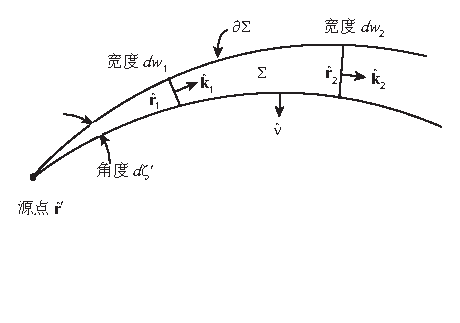
\includegraphics{../figures/chap16/fig01.eps}
\end{center}
\caption[tube]{\label{fig:16.tube}
Schematic depiction of a Love or Rayleigh ray tube on the surface of the unit
sphere $\Omega$.  The tube subtends a differential takeoff angle
\index{takeoff angle}%
$d\zeta'$ at the source point $\brh'$.
The unit wavevectors at the two points $\brh_1$ and $\brh_2$ are
$\bkh_1$ and $\bkh_2$, respectively.  The differential
ray-tube widths $dw_1$ and $dw_2$ at these two points
are measured in radians on $\Omega$.}
\end{figure}
\index{conservation!of surface-wave energy|)}%
\index{energy!conservation of!surface-wave|)}%

\subsection{Surface-wave normalization}
\index{normalization condition!surface waves|(}%
\index{surface-wave normalization condition|(}%

Thus far in this book, we have adhered strictly to the
eigenfunction normalization convention $I_1=1$.  Now,
following Tromp \& Dahlen (\citeyear{tromp&dahlen92b}),
we shall depart from this, requiring instead that
\eq \label{16.newnormal}
c\hspace{0.2 mm}CI_1=1.
\en
This new eigenfunction normalization relation is
particularly convenient in the JWKB analysis of
Love and Rayleigh surface waves on a laterally
heterogeneous Earth.  The amplitude variation
law~(\ref{16.uglyamp}) is simplified to
\eq \label{16.prettyamp}
\frac{A_2}{A_1}=\left(\frac{k_2}{k_1}\right)^{-1/2}
\left|\frac{dw_2}{dw_1}\right|^{-1/2}.
\en
Apart from a constant factor, the
normalization~(\ref{16.newnormal}) is identical
to that introduced by Snieder \& Nolet
(\citeyear{snieder&nolet87}).  They show
that it simplifies the expression for the
surface-wave Green tensor $\bG(\bx,\bx';\om)$
and moment-tensor response $\ba(\bx,\om)$
on a spherically symmetric Earth; in particular,
the reciprocal wave-speed product $(c\hspace{0.3 mm}C)^{-1}$
is replaced by unity in both~(\ref{11.dubsum})
and~(\ref{11.accsum}).
\index{normalization condition!surface waves|)}%
\index{surface-wave normalization condition|)}%

\renewcommand{\thesubsection}{$\!\!\!\raise1.3ex\hbox{$\star$}\!\!$
\arabic{chapter}.\arabic{section}.\arabic{subsection}}
\subsection{Ray-tube width}
\index{ray-tube width|(}%
\renewcommand{\thesubsection}{\arabic{chapter}.\arabic{section}.\arabic{subsection}}

Explicit expressions for the ray-tube width ratio
$dw_2/\hspace{-0.2 mm}dw_1$ can be obtained using
arguments analogous to those in Section~15.4.2.
We shall not repeat the derivations,
which are straightforward, but
simply give the surface-wave analogues
of equations~(\ref{15.kline4})
and~(\ref{15.dSigeqn2}) here:
\eq \label{16.dw}
\frac{dw_2}{dw_1}=\exp\left(\int_{\Delta_1}^{\Delta_2}
\bdel_1\cdot\bkh\,d\Delta\right),
\en
\eq \label{16.dwagain}
\frac{k_2}{k_1}\frac{dw_2}{dw_1}=
\exp\left(\int_{\sigma_1}^{\sigma_2}
\bdel_1\cdot\bk\,d\sigma\right).
\en
The surface divergences in the integrands
of~(\ref{16.dw}) and~(\ref{16.dwagain}) are related
by $\bdel_1\cdot\bk=\bdel_1\cdot(k\bkh)
=k\bdel_1\cdot\bkh+d(\ln k)/d\sigma$.
\index{ray-tube width|)}%

\subsection{Point-source Jacobian}
\index{Jacobian!point-source!surface waves|(}%
\index{point-source Jacobian!surface waves|(}%
\label{section:16.4.4}

The family of surface-wave rays shot from a source point $\brh'$
can be parameterized in terms of a single variable, which we shall
denote by $\zeta'$.  We shall eventually take this ray parameter
to be the takeoff azimuthal angle $0\leq\zeta'\leq 2\pi$, measured
\index{takeoff angle}%
counterclockwise from due south, in accordance with the convention
established for body waves in Section~\ref{section:15.8}.  For the time being,
however, this particular identification is not important; it is
sufficient to regard $\zeta'$ as a label that distinguishes the
various rays shot from $\brh'$.  The partial derivative $\p_{\zeta'}\brh
=(\p\brh/\p\zeta^{\prime})_{\sigma}$ is a tangent vector upon
$\Omega$ that lies within the wavefront passing through the point
$\brh$; the condition that guarantees this is
\eq \label{16.dzetaperp}
\bkh\cdot\p_{\zeta'}\brh=k_{\gamma}(\p_{\zeta'}x^{\gamma})=0.
\en
We define a two-dimensional {\em point-source Jacobian\/} by analogy
\index{point-source Jacobian!surface waves}%
\index{Jacobian!point-source!surface waves}%
with~(\ref{15.Jacob1}):
\eqa \label{16.Jacob1} \lefteqn{
J=\frac{\p(x^1,x^2)}{\p(\sigma,\zeta')}=
\frac{\p x^1}{\p\sigma}\frac{\p x^2}{\p\zeta'}
-\frac{\p x^1}{\p\zeta'}\frac{\p x^2}{\p\sigma}} \nonumber \\
&&\mbox{}\hspace{-4.5 mm}=(g^{11}k_1+g^{12}k_2)(\p_{\zeta'}x^2)
-(\p_{\zeta'}x^1)(g^{21}k_1+g^{22}k_2).
\ena
The amplitude variation along a ray can be expressed in terms of the
Jacobian~(\ref{16.Jacob1}) by an application of Smirnov's lemma
analogous to that in Section~15.4.4.  Invoking the new eigenfunction
normalization~(\ref{16.newnormal}), we rewrite the surface-wave
transport relation~(\ref{16.gtransport}) in the form
\eq
\bdel_1\cdot(A^2\bk)=0,
\en
or, equivalently,
\eq \label{16.trnewnorm}
\frac{d}{d\sigma}\ln A^2=-\bdel_1\cdot\bk.
\en
{\em Smirnov's lemma on a curved surface\/} stipulates that
\index{Smirnov's lemma}%
\eq \label{16.Smirnov}
\frac{d}{d\sigma}\ln(gJ)=\bdel_1\cdot\bk\quad
\mbox{whenever}\quad\frac{d\brh}{d\sigma}=\bk.
\en
The quantity $g$ (not to be confused with the acceleration
of gravity) is related to the covariant and contravariant
components of the metric tensor $\bg=\bI-\brh\brh$ on
the surface $\Omega$ by
\eq \label{16.gdef}
g=\sqrt{{\rm det}\,g_{\alpha\beta}}=\frac{1}
{\sqrt{{\rm det}\,g^{\alpha\beta}}}.
\en
It may be readily verified by expansion of the
respective determinants that
\eq \label{16.Jgident}
\frac{d}{d\sigma}\ln J=\frac{\p k^{\gamma}}
{\p x^{\gamma}},\qquad\frac{d}{d\sigma}\ln g
=\half g^{\alpha\beta}\left(\frac{dg_{\alpha\beta}}
{d\sigma}\right).
\en
To prove~(\ref{16.Smirnov}) we combine the results~(\ref{16.Jgident}):
\eqa \label{16.Smirnpr} \lefteqn{
\frac{d}{d\sigma}\ln(gJ)=\frac{\p k^{\gamma}}
{\p x^{\gamma}}+\half g^{\alpha\beta}\left(\frac{dg_{\alpha\beta}}
{d\sigma}\right)} \nonumber \\
&&\mbox{}\hspace{8.1 mm}=\frac{\p k^{\gamma}}
{\p x^{\gamma}}+\half g^{\alpha\beta}\left(\frac{dg_{\alpha\beta}}
{d x^{\gamma}}\right)k^{\gamma} \nonumber \\
&&\mbox{}\hspace{8.1 mm}=\half g^{\alpha\beta}
\frac{d}{d x^{\gamma}}(g_{\alpha\beta}
k^{\gamma})=\bdel_1\cdot\bk,
\ena
where we have used $g^{\alpha\beta}g_{\alpha\beta}=2$
in the penultimate step and~(\ref{A.divneed16})
to obtain the final identification.
Comparison of equations~(\ref{16.trnewnorm}) and~(\ref{16.Smirnov})
now gives a result analogous to~(\ref{15.gtrans3}):
\eq \label{16.AandJ}
\frac{d}{d\sigma}\ln(gJA^2)=0.
\en
Equation~(\ref{16.AandJ}) enables us to express the
amplitude ratio~(\ref{16.prettyamp}) in terms of a
ratio of Jacobians:
\eq \label{16.prettyA2}
\frac{A_2}{A_1}=\left(\frac{g_2}{g_1}\right)^{-1/2}
\left|\frac{J_2}{J_1}\right|^{-1/2}.
\en
In fact, the differential ray-tube width $dw$ and the Jacobian
$J$ are related everywhere along a ray by an equation analogous
to~(\ref{15.Jacob3}):
\eq \label{16.dwJrel}
k\,dw=gJ\,d\zeta'.
\en
The amplitude variation laws~(\ref{16.prettyamp}) and~(\ref{16.prettyA2})
are equivalent by virtue of~(\ref{16.dwJrel}).
\index{Jacobian!point-source!surface waves|)}%
\index{point-source Jacobian!surface waves|)}%

\subsection{Geometrical spreading factor}
\index{geometrical spreading factor!surface waves|(}%

It is convenient to define a {\em geometrical spreading factor\/}
$S(\brh,\brh')$ on the unit sphere $\Omega$ by
\eq \label{16.Sdef}
S=|dw|/d\zeta'.
\en
The numerator $|dw|$ in~(\ref{16.Sdef}) is the absolute
differential width of a ray tube at the receiver $\brh$,
whereas the denominator $d\zeta'$ is the differential
solid angle subtended by this ray tube at the source
$\brh'$, as illustrated in Figure~\ref{fig:16.tube}.
On a spherically symmetric Earth, this ratio reduces
to $S=|\sin\Delta|$, where $\Delta$ is the total
propagation distance around a great-circular orbit.
The spreading factor $S$ and the Jacobian $J$ are
related by
\eq \label{16.relJS}
kS=g|J|.
\en
We can express the differential width of a ray tube
in a manner analogous to~(\ref{15.Backus1}):
\eq \label{16.recip1}
dw=\bkh\cdot(\brh\times\p_{\zeta'}\brh)\,d\zeta'.
\en
The geometrical spreading factor~(\ref{16.Sdef})
is as a result given by
\eq \label{16.recip2}
S=|\bkh\cdot(\brh\times\p_{\zeta'}\brh)|
=|(\bkh\times\brh)\cdot\p_{\zeta'}\brh|.
\en
It is readily demonstrated that
$(\bkh^{\raise-.65ex\hbox{$\scriptstyle\prime$}}\times\brh')
\cdot\p_{\zeta'}\bkh^{\raise-.65ex\hbox{$\scriptstyle\prime$}}
=-1$. \vspace{-0.4 mm}
The derivative of the takeoff wavevector $\p_{\zeta'}\bk'
=k^{\prime}\p_{\zeta'}\bkh^{\raise-.65ex\hbox{$\scriptstyle\prime$}}$
can be written in terms of the phase difference $\psi(\brh,\brh')
=\psi(\brh',\brh)$ between the source and receiver in the form
$\p_{\zeta'}\bk'=\p_{\zeta'}\brh\cdot
\bdel_1\bdel_1^{\prime}\psi$.
Upon combining these results
and invoking~(\ref{16.dzetaperp}) we find that
\eq \label{16.recip3}
k^{\prime\,-1}
[(\bkh\times\brh)\cdot\p_{\zeta'}\brh]
\,[(\bkh\times\brh)\cdot
\bdel_1\bdel_1^{\prime}\psi\cdot
(\bkh^{\raise-.65ex\hbox{$\scriptstyle\prime$}}\times\brh')]=-1.
\en
Inserting the geometrical identity~(\ref{16.recip3}) into~(\ref{16.recip2})
we obtain an alternative representation of the spreading factor
analogous to~(\ref{15.Backus6}):
\eq \label{16.recip4}
kS=kk'|(\bkh\times\brh)\cdot
\bdel_1\bdel_1^{\prime}\psi\cdot
(\bkh^{\raise-.65ex\hbox{$\scriptstyle\prime$}}\times\brh')|^{-1}.
\en
The right side of equation~(\ref{16.recip4}) is invariant
under an interchange of the source and receiver:
\eq \label{16.recip5}
\brh\rightarrow\brh',\qquad\brh'\rightarrow\brh,\qquad
\hat{\bk}\rightarrow-\bkh^{\raise-.65ex\hbox{$\scriptstyle\prime$}},\qquad
\bkh^{\raise-.65ex\hbox{$\scriptstyle\prime$}}\rightarrow-\hat{\bk}.
\en
It follows that $S$ satisfies the
\index{reciprocity!geometrical spreading factor}%
{\em dynamical reciprocity relation\/}
\eq \label{16.RECIP}
k(\brh)S(\brh,\brh')=k(\brh')S(\brh',\brh).
\en
Equation~(\ref{16.RECIP}) is the surface-wave analogue
of~(\ref{15.Backus8}); this result was first established
by Woodhouse \& Wong (\citeyear{woodhouse&wong86}).
\index{geometrical spreading factor!surface waves|)}%

\subsection{Dynamical ray tracing}
\index{dynamical ray tracing!surface waves|(}%
\index{ray tracing!dynamical|(}%

In order to calculate the Jacobian~(\ref{16.Jacob1})
we need to know the partial derivatives
$\p_{\zeta'}x^1$ and $\p_{\zeta'}x^2$ along a ray.
These derivatives satisfy a linear system of equations
obtained by partial differentiation of~(\ref{16.rayeqns}):
\eq
\frac{d}{d\sigma}\left(\frac{\p x^{\gamma}}{\p\zeta'}\right)
=\left(\frac{\p g^{\gamma\eta}}{\p x^\alpha}\right)
k_{\eta}\left(\frac{\p x^{\alpha}}{\p\zeta'}\right)
+g^{\gamma\eta}\left(\frac{\p k_{\eta}}{\p\zeta'}\right),
\en
\eqa
\lefteqn{
\frac{d}{d\sigma}\left(\frac{\p k_{\gamma}}{\p\zeta'}\right)
=-\half\left(\frac{\p^2g^{\alpha\beta}}
{\p x^{\gamma}\p x^{\eta}}\,k_{\alpha}k_{\beta}
-\frac{\p^2 k^2}{\p x^{\gamma}\p x^{\eta}}
\right)\left(\frac{\p x^{\eta}}{\p\zeta'}\right)} \nonumber \\
&&\mbox{}\qquad\qquad\hspace{2.0 mm}
-\left(\frac{\p g^{\alpha\beta}}{\p x^{\gamma}}\right)
k_{\alpha}\left(\frac{\p k_{\beta}}{\p\zeta'}\right).
\ena
This system of four equations must be solved
subject to the point-source initial conditions
\eq
\partial_{\zeta'}x^{\gamma}(0)=0,
\qquad
\partial_{\zeta'}k_{\gamma}(0)=
\partial_{\zeta'}k_{\gamma}^{\prime}.
\en
The two quantities $\brh+\p_{\zeta'}\brh$ and $\bk+\p_{\zeta'}\bk$ are
the position and wavevector along a {\em neighboring or paraxial ray\/}.
\index{neighboring ray}%
\index{paraxial ray}%
\index{dynamical ray tracing!surface waves|)}%
\index{ray tracing!dynamical|)}%

\subsection{Maslov index}
\index{Maslov index!surface waves|(}%
\index{index!Maslov|(}%
\label{16.sec.Maslov}

Singular points on $\Omega$ where neighboring
surface-wave rays cross are known as {\em caustics\/},
\index{caustic!surface waves}%
just as in the case of body waves.  Caustic passages
can be monitored by keeping track of sign changes in
the Jacobian~(\ref{16.Jacob1}):
\eq \label{16.causticdef}
\mbox{caustic:}\quad J=0.
\en
We again introduce the {\em Maslov index\/} $M$, a positive
integer counter that is incremented by one each time that
the condition~(\ref{16.causticdef}) is satisfied.  The number
of caustic passages is invariant under an interchange of the
\index{reciprocity!Maslov index}%
\index{Maslov reciprocity principle}%
source and receiver:
\eq \label{16.Mrecip}
M(\brh,\brh')=M(\brh',\brh).
\en
On a spherical Earth the caustics are points situated at
the source $\brh'$ and its antipode $-\brh'$.  The rays
shot from $\brh$ likewise exhibit caustics at $\pm\brh$.
No matter how many full or partial orbits a ray makes,
it is obvious that the reciprocity relation~(\ref{16.Mrecip})
is always satisfied. More generally, on a slightly
heterogeneous Earth, the caustics are closed,
multi-cusped curves in the vicinity of the source
and its antipode, as we illustrate in
Section~16.6.7.  For a small
enough perturbation, the relation~(\ref{16.Mrecip})
is still obvious; in fact, it pertains to any smooth
Earth model, even one with with large lateral variations
in surface-wave phase speed $c$.  The phase of a Love or Rayleigh
wave undergoes a non-geometrical $\pi/2$ phase advance
upon every passage through a near-source or near-antipodal
caustic.  The existence of this so-called {\em polar phase shift\/}
\index{polar phase shift}%
\index{phase shift!polar}%
was first pointed out on a spherical Earth by Brune, Nafe \& Alsop
(\citeyear{brune&al61}).
\index{Maslov index!surface waves|)}%
\index{index!Maslov|)}%

\subsection{Anelasticity}
\index{anelasticity!surface-wave|(}%
\index{attenuation!surface-wave|(}%

It is straightforward to incorporate the effects of slight,
laterally variable anelasticity into surface-wave JWKB theory.
As usual, we replace the perfectly elastic incompressibility
and rigidity by complex, frequency-dependent moduli:
\eq \label{16.kappadef}
\kappa\rightarrow\kappa_0[1+\twoinvpi Q_{\kappa}^{-1}
\ln(\om\hspace{-0.2 mm}/\hspace{-0.2 mm}\om_0)]
+i\kappa_0Q_\kappa^{-1},
\en
\eq \label{16.mudef}
\mu\rightarrow\mu_0[1+\twoinvpi Q_{\mu}^{-1}
\ln(\om\hspace{-0.2 mm}/\hspace{-0.2 mm}\om_0)]
+i\mu_0Q_\mu^{-1},
\en
where a subscript zero denotes evaluation at the reference
frequency $\om_0$.  The real parts of~(\ref{16.kappadef})
and~(\ref{16.mudef}) are the real incompressibility and
rigidity ``seen'' by a monochromatic Love or Rayleigh wave
of angular frequency $\omega$.  We account for the effect
of this anelastic dispersion upon the local real wavenumber
$k$ and the local radial eigenfunctions $U$, $V$, $P$ and
$W$ by incorporating these frequency-dependent moduli
directly into the defining equations~(\ref{16.W})
and~(\ref{16.U})--(\ref{16.P}) and associated boundary
conditions~(\ref{16.T1})--(\ref{16.T2})
and~(\ref{16.RS1})--(\ref{16.P1}).
The effect of the imaginary perturbations
$i\kappa_0Q_{\kappa}^{-1}$ and $i\mu_0Q_{\mu}^{-1}$
upon $U$, $V$, $W$ and $P$ will be ignored;
their effect upon the local wavenumber can be
found by perturbing the local dispersion
relations~(\ref{16.locdisL}) and~(\ref{16.locdisR}).
Rayleigh's principle is the critical cog in the
analysis, as in Sections~9.2 and~9.7; the only difference
is that we now perturb $k$ at fixed $\omega$ rather
than $\omega$ at fixed $k$.  The distinction between
these two types of perturbations is elaborated upon
in Section~11.8.  Writing the imaginary wavenumber
perturbation in the form $k\rightarrow k-i
\hspace{0.7 mm}\delta k$, we find, in terms
of the present notation, that
\eq \label{16.LRQ}
\delta k_{\rm L}=\frac{k_{\rm L}^2\delta I_2
+\delta I_3}{2k_{\rm L}I_2},\qquad
\delta k_{\rm R}=\frac{k_{\rm R}^2\delta I_2^{\prime}+
k_{\rm R}\delta I_3^{\prime}+\delta I_4^{\prime}}
{2k_{\rm R}I_2^{\prime}+I_3^{\prime}},
\en
where the subscripts L and R distinguish
Love and Rayleigh waves, respectively.
The perturbed radial integrals $\delta I_2$,
$\delta I_3$ and $\delta I_2^{\prime}$,
$\delta I_3^{\prime}$, $\delta I_4^{\prime}$
in equations~(\ref{16.LRQ}) are given by
\eq \label{16.dI2L}
\delta I_2=\int_0^a\mu_0Q_{\mu}^{-1} W^2\,dr,
\en
\eq \label{16.dI3L}
\delta I_3=\int_0^a\mu_0Q_{\mu}^{-1}
[(\p_rW-r^{-1}W)^2-2r^{-2}W^2]\,r^2dr,
\en
\eq \label{16.dI2R}
\delta I_2^{\prime}=\int_0^a[\mu_0Q_{\mu}^{-1}
U^2+(\kappa_0Q_{\kappa}^{-1}+\fourthirds\mu_0Q_{\mu}^{-1})V^2]\,dr,
\en
\eqa
\lefteqn{\delta I_3^{\prime}=\int_0^a[\fourthirds\mu_0Q_{\mu}^{-1} V
(\p_rU-r^{-1}U)-2\kappa_0Q_{\kappa}^{-1} V(\p_rU+2r^{-1}U)} \nonumber \\
&&\qquad\mbox{}+2\mu_0Q_{\mu}^{-1}U(\p_rV-r^{-1}V)]\,rdr,
\ena
\eqa  \label{16.dI4R}
\lefteqn{\delta I_4^{\prime}=
\int_0^a[(\kappa_0Q_{\kappa}^{-1}(\p_rU+2r^{-1}U)^2
+\fourthirds\mu_0Q_{\mu}^{-1}(\p_rU-r^{-1}U)^2} \nonumber \\
&&\qquad\mbox{}+\mu_0Q_{\mu}^{-1}(\p_rV-r^{-1}V)^2
-2\mu_0Q_{\mu}^{-1} r^{-2}V^2]\,r^2dr.
\ena
It is conventional to express the perturbations~(\ref{16.LRQ})
in terms of the {\em temporal quality factors\/}
\index{temporal quality factor}%
\index{quality factor!temporal}%
\index{Q@{\em Q}!temporal}%
of the associated standing waves.  Making use
of equations~(\ref{16.Lgrvel}) and~(\ref{16.Rgrvel})
we find that $\delta k=(ck)/(2CQ)$, where
\eq \label{16.LRQ2}
Q_{\rm L}^{-1}=\frac{k_{\rm L}^2\delta I_2
+\delta I_3}{\om^2I_{1{\rm L}}},\qquad
Q_{\rm R}^{-1}=\frac{k_{\rm R}^2\delta I_2^{\prime}+
k_{\rm R}\delta I_3^{\prime}+\delta I_4^{\prime}}
{\om^2I_{1{\rm R}}}.
\en
The upshot is an exponential decay
of the wave amplitude with angular
distance from the source, of the form
\eq \label{16.kpertQ}
\exp(-ik\Delta)\rightarrow
\exp(-ik\Delta)\exp(-\om\Delta/2CQ).
\en
It is readily verified that the local Love and Rayleigh
\index{quality factor!local}%
\index{local quality factor}%
\index{Q@{\em Q}!local}%
\index{local {\em Q}}%
quality factors~(\ref{16.LRQ2})
are identical to~(\ref{9.anel7}).  The factor $C$
appears in the denominator of~(\ref{16.kpertQ})
because the wave energy---which is what is being
dissipated---propagates with the group speed.
Strictly speaking, $C$ should be calculated in
the reference-frequency Earth model, with laterally
variable elastic parameters $\kappa_0$ and $\mu_0$,
for consistency with~(\ref{16.dI2L})--(\ref{16.dI4R});
we omit the customary subscript 0 used to denote
this, for simplicity.  In practice, it is possible
to use the speed $C$ at which a monochromatic wavegroup
of frequency $\omega$ actually
propagates, with negligible error.
\index{anelasticity!surface-wave|)}%
\index{attenuation!surface-wave|)}%
\index{amplitude!surface-wave|)}%
\index{surface-wave amplitude|)}%

\section{JWKB Response}
\index{response!surface-wave|(}%
\index{surface-wave response|(}%

All of the ingredients needed to express the JWKB
surface-wave response of a laterally heterogeneous
Earth to a point source have now been assembled.
We derive the JWKB Green tensor $\bG(\bx,\bx';\om)$
and the acceleration response $\ba(\bx,\om)$ to a
moment-tensor source in the next two sections.

\subsection{Green tensor}
\index{Green tensor!surface-wave|(}%
\index{tensor!Green!surface-wave|(}%

We begin by rewriting the far-field surface-wave Green
tensor~(\ref{11.dubsum}) on a spherically symmetric Earth,
using the new eigenfunction normalization~(\ref{16.newnormal}):
\eqa \label{16.spherG}
\lefteqn{
\bG_{\rm spher}(\bx,\bx';\om)=\sum_{\rm modes}\,\sum_{\rm rays}\hspace{1.0 mm}
(8\pi k|\sin\Delta|)^{-1/2}} \\
&&\mbox{}\times[\brh U-i\bkh V+i(\brh\times\bkh)W]
[\brh' U'+i\bkh^{\raise-.65ex\hbox{$\scriptstyle\prime$}}
V'-i(\brh'\times\bkh^{\raise-.65ex\hbox{$\scriptstyle\prime$}})W']  \nonumber \\
&&\mbox{}\qquad\times\exp i\left(-k\Delta+M
\pi/2-\pi/4\right)\exp(-\om\Delta/2CQ). \nonumber
\ena
The first sum in~(\ref{16.spherG}) is over the various
surface-wave {\em modes\/} or dispersion branches,
whereas the second is over the multi-orbit {\em rays\/}
or sequential arrivals, as illustrated in Figure~11.3.
Both Love and Rayleigh waves are included in the double
sum; $U=V=0$ for the former, whereas $W=0$ for the latter.
The Maslov index $M$ is simply $s-1$, where $s=1,2,3,\ldots$
is the numerical order of the arrival.  We can write the JWKB
Green tensor on a laterally heterogeneous Earth in a form
analogous to~(\ref{16.spherG}):
\eqa \label{16.ansatzG}
\lefteqn{
\bG(\bx,\bx';\om)=\sum_{\rm modes}\,\sum_{\rm rays}\hspace{1.0 mm}
(kS)^{-1/2}[\brh U-i\bkh V+i(\brh\times\bkh)W]\,\bA'
} \nonumber \\
&&\mbox{}\times
\exp i\left(-\int_0^\Delta k\,d\Delta+M\frac{\pi}{2}\right)
\exp\left(-\om\int_0^\Delta\frac{d\Delta}{2CQ}\right),
\ena
where we seek to determine the unknown vector $\bA'$.
The factor $(kS)^{-1/2}$ accounts for amplitude variations
along the rays due to geometrical spreading, in accordance
with the elastic energy-conservation law~(\ref{16.prettyamp})
and the definition~(\ref{16.Sdef}).  We find $\bA'$ by
matching the $s=1$ ray in~(\ref{16.ansatzG}) to that
in~(\ref{16.spherG}) in the vicinity of the source
$\brh'$, where the Earth model may be considered
locally homogeneous.  The near-source geometrical
spreading factor is simply $S\rightarrow\sin\Delta$,
so that
\eq
\bA'=(1/8\pi)^{1/2}
[\brh' U'+i\bkh^{\raise-.65ex\hbox{$\scriptstyle\prime$}}
V'-i(\brh'\times\bkh^{\raise-.65ex\hbox{$\scriptstyle\prime$}})W']
\exp(-i\pi/4).
\en
The JWKB Green tensor on a laterally heterogeneous Earth is
therefore
\eqa \label{16.G}
\lefteqn{
\bG(\bx,\bx';\om)=\sum_{\rm modes}\,\sum_{\rm rays}\hspace{1.0 mm}
(8\pi kS)^{-1/2}} \nonumber \\
&&\mbox{}\!\!\!\!\!\!\!\!
\times[\brh U-i\bkh V+i(\brh\times\bkh)W]
[\brh' U'+i\bkh^{\raise-.65ex\hbox{$\scriptstyle\prime$}}
V'-i(\brh'\times\bkh^{\raise-.65ex\hbox{$\scriptstyle\prime$}})W']  \nonumber \\
&&\mbox{}\!\!\!\!\!\!\!\!
\times\exp i\left(-\int_0^\Delta k\,d\Delta+M
\frac{\pi}{2}-\frac{\pi}{4}\right)
\exp\left(-\om\int_0^\Delta\frac{d\Delta}{2CQ}\right).
\ena
The JWKB response~(\ref{16.G}) is invariant
under an interchange~(\ref{16.recip5}) of the
\index{reciprocity!surface waves}%
source and receiver,
\eq
\bG(\bx,\bx';\om)=\bG^{\rm T}(\bx',\bx;\om),
\en
by virtue of the geometrical reciprocity
relations~(\ref{16.RECIP}) and~(\ref{16.Mrecip}).
\index{Green tensor!surface-wave|)}%
\index{tensor!Green!surface-wave|)}%

\subsection{Moment-tensor response}
\index{moment-tensor response!surface waves|(}%
\index{response!moment-tensor|(}%

The acceleration response to a frequency-dependent moment-tensor
source $\bM(\om)$ at a hypocentral location $\bx_{\rm s}$ can be
expressed in terms of the Green tensor~(\ref{16.G}) in the form
\eq
\ba(\bx,\om)=i\om\bM\!:\!\bdel_{\!\rm s}
\bG^{\rm T}(\bx,\bx_{\rm s};\om).
\en
To lowest order, the gradient $\bdel_{\!\rm s}$
with respect to the source
coordinates $\bx_{\rm s}$ acts only upon
the oscillatory path integral  \vspace{-0.6 mm}
$\exp(-i\int_0^{\raise-.25ex\hbox{$\scriptstyle\Delta$}}
k\,d\Delta)$ and the polarization vector $\brh_{\rm s}U_{\rm s}
+i\bkh_{\rm s}V_{\rm s}-i(\brh_{\rm s}\times\bkh_{\rm s})W_{\rm s}$
of the surface wave leaving the source.
\index{surface-wave polarization}%
\index{polarization!surface-wave}%
We can write the surface-wave
acceleration upon a laterally heterogeneous Earth in the form
\eqa \label{16.accsum}
\lefteqn{
\ba(\bx,\om)=i\om\sum_{\rm modes}\,\sum_{\rm rays}\hspace{1.0 mm}
(8\pi kS)^{-1/2}[\brh U-i\bkh V+i(\brh\times\bkh)W]}  \nonumber \\
&&\mbox{}
\times(\bM\!:\!\bE_{\rm s}^*)\,\exp i\left(-\int_0^\Delta k\,d\Delta+M
\frac{\pi}{2}-\frac{\pi}{4}\right) \nonumber \\
&&\mbox{}\qquad\qquad
\times\exp\left(-\om\int_0^\Delta\frac{d\Delta}{2CQ}\right),
\ena
where the quantity
\eqa \label{16.strain}
\lefteqn{\bE_{\rm s}=\p_rU_{\rm s}\brh_{\rm s}\brh_{\rm s}
+r_{\rm s}^{-1}(U_{\rm s}-k_{\rm s}V_{\rm s})\bkh_{\rm s}\bkh_{\rm s}
+r_{\rm s}^{-1}U_{\rm s}(\brh_{\rm s}\times\bkh_{\rm s})
(\brh_{\rm s}\times\bkh_{\rm s})} \nonumber \\
&&-\half i(\p_rV_{\rm s}-r_{\rm s}^{-1}V_{\rm s}
+k_{\rm s}r_{\rm s}^{-1}U_{\rm s})(\brh_{\rm s}\bkh_{\rm s}
+\bkh_{\rm s}\brh_{\rm s}) \nonumber \\
&&\mbox{}\quad+\half i(\p_rW_{\rm s}-r_{\rm s}
^{-1}W_{\rm s})[\brh_{\rm s}(\brh_{\rm s}\times\bkh_{\rm s})
+(\brh_{\rm s}\times\bkh_{\rm s})\brh_{\rm s}] \nonumber \\
&&\quad\qquad+\half k_{\rm s}r_{\rm s}^{-1}W_{\rm s}
[\bkh_{\rm s}(\brh_{\rm s}\times\bkh_{\rm s})
+(\brh_{\rm s}\times\bkh_{\rm s})\bkh_{\rm s}]
\ena
is the JWKB strain tensor at the source.  The results~(\ref{16.G})
\index{strain tensor!JWKB}%
\index{tensor!JWKB strain}%
and~(\ref{16.accsum}) are identical to the far-field surface-wave
Green tensor~(\ref{11.dubsum}) and moment-tensor
response~(\ref{11.accsum}) on a spherically symmetric Earth,
with the geometrical spreading factor $|\sin\Delta|^{-1/2}$
replaced by $S^{-1/2}$, and the source-to-receiver phase delay
and attenuation $\exp(-ik\Delta)\exp(-\om\Delta/2CQ)$
replaced by $\exp(-i\int_0^{\raise-.25ex\hbox{$\scriptstyle\Delta$}}
k\,d\Delta)\exp(-\om\int_0^{\raise-.25ex\hbox{$\scriptstyle\Delta$}}
d\Delta/2CQ)$.  The strain~(\ref{16.strain}) is identical
to~(\ref{11.strain}) with the wavenumber $k$ replaced by
$k_{\rm s}$ and the ordinary radial derivatives $\dot{U}_{\rm s}$,
$\dot{V}_{\rm s}$, $\dot{W}_{\rm s}$ replaced by
$\p_rU_{\rm s}$, $\p_rV_{\rm s}$, $\p_rW_{\rm s}$.

In preparation for the perturbation theory which we shall present
in Section~\ref{16.sec.raypert}, it is convenient to write the
$\bnuh$ component $a(\om)=\bnuh\cdot\ba(\bx,\om)$
of the acceleration~(\ref{16.accsum}) at the receiver
$\bx$ in the form
\eq \label{16.TDneed1}
a=\sum_{\rm modes}\,\sum_{\rm rays}A\exp(-i\psi),
\en
where
\eq \label{16.TDneed2}
A=A_{\rm r}A_{\rm p}A_{\rm s},\qquad
\psi=\psi_{\rm r}+\phi_{\rm p}+\psi_{\rm s}.
\en
The amplitudes $A_{\rm s}$, $A_{\rm p}$,
$A_{\rm r}$ and phases $\psi_{\rm s}$, $\phi_{\rm p}$,
$\psi_{\rm r}$ are given explicitly by
\eq \label{16.dAs}
A_{\rm s}\exp(-i\psi_{\rm s})=i\om(\bM\!:\!\bE_{\rm s}^*)\exp(-i\pi/4),
\en
\eqa \label{16.dAp} \lefteqn{
A_{\rm p}\exp(-i\psi_{\rm p})=
(8\pi kS)^{-1/2}\exp i\left(-\int_0^\Delta
k\,d\Delta+M\frac{\pi}{2}\right)} \nonumber \\
&&\mbox{}\qquad\qquad\times
\exp\left(-\int_0^\Delta\frac{\omega}{2CQ}\,d\Delta\right),
\ena
\eq \label{16.dAr}
A_{\rm r}\exp(-i\psi_{\rm r})=\bnuh\cdot[\brh U-i\bkh V+i(\brh\times\bkh)W].
\en
The subscripts ${\rm s}$, ${\rm p}$
and ${\rm r}$ label contributions associated with the
{\em source\/}, {\em path\/} and {\em receiver\/},
\index{perturbation!source}%
\index{perturbation!path}%
\index{perturbation!receiver}%
\index{anomaly!source}%
\index{anomaly!path}%
\index{anomaly!receiver}%
respectively.  For Love waves, the contraction of
the moment tensor $\bM$ and the conjugate source
strain $\bE_{\rm s}^*$ is given by
\eqa  \label{16.MEsL}
\lefteqn{
\bM\!:\!\bE_{\rm s}^*=i(\p_rW_{\rm s}
-r_{\rm s}^{-1}W_{\rm s})(M_{r\theta}\sin\zeta_{\rm s}
-M_{r\phi}\cos\zeta_{\rm s})} \nonumber \\
&&\mbox{}-k_{\rm s}r_{\rm s}^{-1}W_{\rm s}[\half(M_{\theta\theta}
-M_{\phi\phi})\sin 2\zeta_{\rm s}-M_{\theta\phi}\cos 2\zeta_{\rm s}],
\ena
whereas for Rayleigh waves it is
\eqa \label{16.MEsR}
\lefteqn{
\bM\!:\!\bE_{\rm s}^*=M_{rr}\p_rU_{\rm s}
+(M_{\theta\theta}+M_{\phi\phi})
r_{\rm s}^{-1}(U_{\rm s}-\half k_{\rm s}V_{\rm s})} \nonumber \\
&&\mbox{}+i(\p_rV_{\rm s}-r_{\rm s}^{-1}V_{\rm s}
+k_{\rm s}r_{\rm s}^{-1}U_{\rm s})(M_{r\phi}\sin\zeta_{\rm s}
+M_{r\theta}\cos\zeta_{\rm s}) \nonumber \\
&&\mbox{}-k_{\rm s}r_{\rm s}^{-1}V_{\rm s}
[M_{\theta\phi}\sin 2\zeta_{\rm s}
+\half(M_{\theta\theta}-M_{\phi\phi})\cos 2\zeta_{\rm s}].
\ena
The quantities $M_{rr}$, $M_{r\theta}$, $M_{r\phi}$,
$M_{\theta\theta}$, $M_{\theta\phi}$, $M_{\phi\phi}$
are the six independent spherical polar components of $\bM$,
as displayed in equation~(\ref{5.Mmatconv}),
and the angle $0\leq \zeta_{\rm s}\leq 2\pi$
is the takeoff azimuth
\index{takeoff angle}%
of the surface-wave ray path on the unit sphere $\Omega$,
measured counterclockwise from due south at the earthquake
epicenter $\brh_{\rm s}$.  The source term
\eqa \label{16.radpat} \lefteqn{
A_{\rm s}\exp(-i\psi_{\rm s})
=\om\big\{[M_{rr}\p_rU_{\rm s}+(M_{\theta\theta}+M_{\phi\phi})
r_{\rm s}^{-1}(U_{\rm s}-\half k_{\rm s}V_{\rm s})]e^{i\pi/4}} \nonumber \\
&&\mbox{}-(\p_rV_{\rm s}-r_{\rm s}^{-1}V_{\rm s}
+k_{\rm s}r_{\rm s}^{-1}U_{\rm s})
(M_{r\phi}\sin\zeta_{\rm s}+M_{r\theta}
\cos\zeta_{\rm s})e^{-i\pi/4} \nonumber \\
&&\mbox{}-k_{\rm s}r_{\rm s}^{-1}
V_{\rm s}[M_{\theta\phi}\sin 2\zeta_{\rm s}+
\half( M_{\theta\theta}-M_{\phi\phi})
\cos 2\zeta_{\rm s}]e^{i\pi/4} \nonumber \\
&&\mbox{}-(\p_rW_{\rm s}-r_{\rm s}^{-1}W_{\rm s})
(M_{r\theta}\sin\zeta_{\rm s}-M_{r\phi}
\cos\zeta_{\rm s})e^{-i\pi/4} \\
&&\mbox{}-k_{\rm s}r_{\rm s}^{-1}W_{\rm s}[\half(M_{\theta\theta}
-M_{\phi\phi})\sin 2\zeta_{\rm s}-
M_{\theta\phi}\cos 2\zeta_{\rm s}]e^{i\pi/4}\big\} \nonumber
\ena
is the {\em complex Love or Rayleigh radiation pattern\/},
\index{radiation pattern!surface-wave}%
\index{surface-wave radiation pattern}%
denoted by the symbol $R(\zeta_{\rm s})$
in Sections~11.4 and~11.7.2.
In fact, equation~(\ref{16.radpat}) is identical
to equation~(11.34), with the great-circular takeoff
azimuths $\Phi$ ($s$ odd) and $\Phi+\pi$ ($s$ even)
replaced by $\zeta_{\rm s}$, and with $k$ and
$\dot{U}_{\rm s}$, $\dot{V}_{\rm s}$, $\dot{W}_{\rm s}$
replaced by $k_{\rm s}$ and $\p_rU_{\rm s}$, $\p_rV_{\rm s}$,
$\p_rW_{\rm s}$.
\index{moment-tensor response!surface waves|)}%
\index{response!moment-tensor|)}%
\index{response!surface-wave|)}%
\index{surface-wave response|)}%

\section{Practical Numerical Implementation}
\label{16.sec.practical}

In this section we outline a practical scheme for
tracing surface-wave rays and computing phase and
amplitude variations along them, analogous to the scheme
for body waves in Section~15.8.  We suppose the
incompressibility, rigidity and density to
be specified functions $\kappa(r,\theta,\phi)$,
$\mu(r,\theta,\phi)$ and $\rho(r,\theta,\phi)$
of the radial distance from the center $r$,
the colatitude $\theta$ and the longitude
$\phi$; likewise, the discontinuity radii are
presumed to be functions of the form $d(\theta,\phi)$.
The spherical polar coordinates of the receiver
$\bx$ are $r,\theta,\phi$ whereas those of the
source $\bx'$ are $r',\theta',\phi'$.

\subsection{Local modes}
\index{local mode|(}%
\index{mode!local|(}%

To compute the JWKB response, we must know the local
displacement eigenfunctions $U$, $V$, $W$ and their
radial derivatives $\p_rU$, $\p_rV$, $\p_rW$ at the
source $\bx'$ and receiver $\bx$.  To find these,
it is necessary to run a modified version of a
normal-mode code such as {\tt MINEOS\/} or {\tt OBANI\/}
\index{MINEOS@\texttt{MINEOS}}%
\index{OBANI@\texttt{OBANI}}%
once at every geographical source and receiver position
$\theta',\phi'$ and $\theta,\phi$.  Figure~\ref{fig:16.locmodes}
shows the depth variation of $U$, $V$, $W$ and $\p_rU$, $\p_rV$,
$\p_rW$ for 165-second fundamental-mode Love and Rayleigh waves
at twenty randomly selected earthquake epicentral locations and
fifty randomly selected GSN station locations on Earth model
SH12WM13 (Su, Woodward \& Dziewonski \citeyear{su&al94}).
The variations in $U$, $\p_rV$ and $W$ in the uppermost
100~km are of order $15\%$; the variations in $\p_rU$, $V$
and  $\p_rW$ between 100~km and 300~km depth can be as
large as $30\%$.  Note that the quantities plotted are
the JWKB-normalized eigenfunctions, which have
$c\hspace{0.3 mm}CI_1=1$ at every point on the unit sphere $\Omega$.
\begin{figure}[!t]
\begin{center}
\scalebox{0.97}{
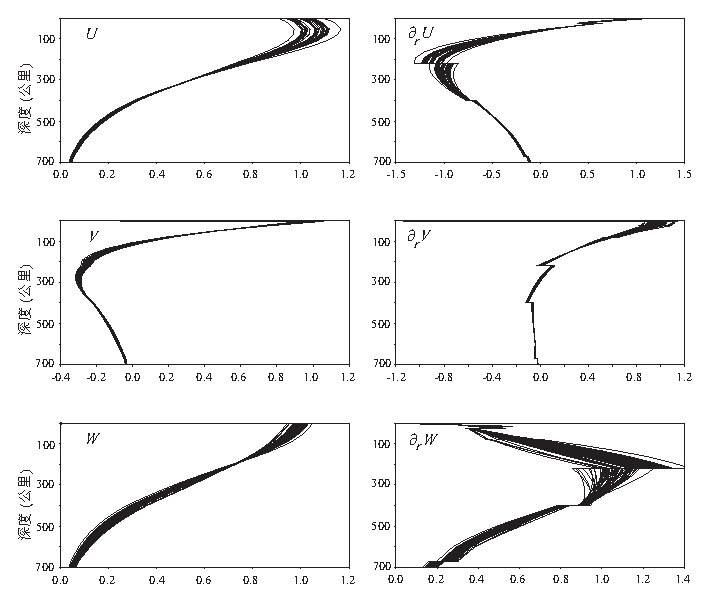
\includegraphics{../figures/chap16/fig02.eps}
}
\end{center}
\caption[locmodes]{\label{fig:16.locmodes}
Depth variation of the eigenfunctions $U$, $V$, $W$
and their radial derivatives $\p_rU$, $\p_rV$, $\p_rW$
at the geographical locations $\theta,\phi$ of twenty
earthquakes and fifty GSN stations on model SH12WM13.
The 165-second fundamental-mode eigenfunctions are
JWKB normalized: $c\hspace{0.2 mm}CI_1=1$.
The Rayleigh-wave quantities $U$, $V$ and $\p_rU$,
$\p_rV$ are scaled such that the average value on
the free surface is unity.  The average values
of the Love-wave quantities $W$ and $\p_rW$ are
scaled to unity on the seafloor and at a depth
of 144~km, respectively.}
\end{figure}

The local dispersion relation $k=k(\theta,\phi,\om)$
and phase speed $c(\theta,\phi,\om)$ must be known at
every point $\theta,\phi$ which may be visited by a
surface wave.  It is generally prohibitive to
call {\tt MINEOS\/} or {\tt OBANI\/} at every step
along a ray path; instead, we resort to the surface-wave
perturbation theory described in Section~11.8.  The
local wavenumber and phase speed are regarded as small
perturbations $k\rightarrow k+\delta k$
and $c\rightarrow c+\delta c$ away from a
spherically averaged Earth.  The perturbations in wavenumber,
phase speed and eigenfrequency at every point on $\Omega$
are related by equation~(\ref{11.threeperts}):
\eq \label{16.threeperts}
\frac{\delta k}{k}
=-\frac{\delta c}{c}=
-\frac{c}{C}\frac{\delta\om}{\om},
\en
where $C$ is the unperturbed group speed.
The resulting local dispersion relation
and phase-speed variations are accurate to first order
in the local structural perturbations
$\delta\hspace{-0.2 mm}\kappa$, $\delta\hspace{-0.2 mm}\mu$,
$\delta\hspace{-0.2 mm}\rho$ and $\delta\hspace{-0.1 mm}d$.
This is an adequate approximation for long-period
($T>100$ s) Love and Rayleigh waves that are not
strongly affected by large lateral variations in
the thickness of the crust.
\index{local mode|)}%
\index{mode!local|)}%

\subsection{Kinematic ray tracing}
\index{ray tracing!kinematic!surface waves|(}%
\index{kinematic ray tracing!surface waves|(}%

To trace surface-wave rays, it is convenient to use the colatitude and
longitude as the generalized coordinates:
\eq
x^1=\theta,\qquad x^2=\phi.
\en
The covariant and contravariant components of the
metric tensor $\bg=\bI-\brh\brh$ are given
in this case by
\eq
g_{\theta\theta}=1,\qquad
g_{\theta\phi}=g_{\phi\theta}=0,\qquad
g_{\phi\phi}=\sin^2\theta,
\en
\eq
g^{\theta\theta}=1,\qquad
g^{\theta\phi}=g^{\phi\theta}=0,\qquad
g^{\phi\phi}=(\sin\theta)^{-2}.
\en
The ray-tracing Hamiltonian~(\ref{16.H}) is therefore
\index{Hamiltonian!surface-wave}%
\index{surface-wave Hamiltonian}%
\eq \label{16.Hagain}
H=\half[k_{\theta}^2+(\sin\theta)^{-2}k_{\phi}^2-k^2(\theta,\phi)]=0.
\en
Hamilton's equations~(\ref{16.hameqn})--(\ref{16.rayeqns})
for the spherical polar Hamiltonian $H(\theta,\phi,k_{\theta},k_{\phi})$ are
\eq \label{16.rays1}
\frac{d\theta}{d\sigma}=k_\theta,
\en
\eq
\frac{d\phi}{d\sigma}=(\sin\theta)^{-2}k_\phi,
\en
\eq
\frac{dk_\theta}{d\sigma}=\half\p_\theta k^2+
\cot\theta(\sin\theta)^{-2}k_\phi^2,
\en
\eq \label{16.rays4}
\frac{dk_\phi}{d\sigma}=\half\p_\phi k^2.
\en
The initial conditions for a ray shot from
$\theta',\phi'$ in a direction $0\leq \zeta'\leq 2\pi$
are $\theta(0)=\theta'$, $\phi(0)=\phi'$ and
$k_\theta(0)=k'\cos\zeta'$, $k_\phi(0)=k'\sin\zeta'$.

The order of the surface-wave
ray-tracing system~(\ref{16.rays1})--(\ref{16.rays4})
can be reduced from four to two, in the same manner that the six body-wave
ray-tracing equations~(\ref{15.LTdrdnu})--(\ref{15.LTdsphidnu}) were
reduced to four equations~(\ref{15.LTeq1})--(\ref{15.LTeq4})
in Section~\ref{15.sec.jeroen1}.  To this end, we introduce
the {\em local azimuth\/} or direction of propagation
\index{azimuth}%
\index{local azimuth}%
$0\leq\zeta\leq 2\pi$ at an arbitrary point $\theta,\phi$
along a ray (see Figure~16.3).
\begin{figure}[!t]
\centering
\begin{tabular}{lr}
\begin{tabular}{l}
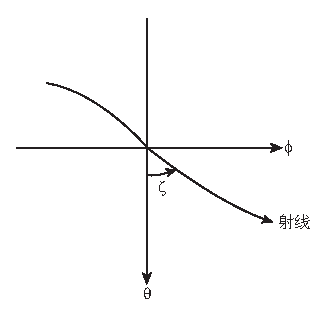
\includegraphics{../figures/chap16/fig03.eps}
\end{tabular}
&
\parbox{4.6cm}{\small
Figure~16.3. The propagation direction of a surface-wave ray
at a point $\theta,\phi$
is specified in terms of the {\em azimuth\/} $0\leq\zeta\leq 2\pi$,
measured counterclockwise from due south.  The takeoff
azimuth at the source $\theta',\phi'$ is simply the primed
value $\zeta'$ of this angle.}
\end{tabular}
\end{figure}
\addtocounter{figure}{1}
The wavevector is given in terms of this azimuthal angle by
\eq \label{16.wavev}
\bk=k\cos\zeta\,\bthetah+k\sin\zeta\,\bphih.
\en
The covariant components of the wavevector,
\eq \label{16.wavevy}
k_\theta=k\cos\zeta,\qquad k_\phi=k\sin\theta\sin\zeta,
\en
are readily shown to satisfy the dispersion relation~(\ref{16.Hagain}).
Using the relations~(\ref{16.wavevy}), we can reduce
the ray-tracing equations~(\ref{16.rays1})--(\ref{16.rays4})
to a system of three ordinary differential equations
governing $\theta$, $\phi$ and $\zeta$:
\eq \label{16.rayd1}
\frac{d\theta}{d\sigma}=k\cos\zeta,
\en
\eq \label{16.rayd2}
\frac{d\phi}{d\sigma}=k(\sin\theta)^{-1}\sin\zeta,
\en
\eq \label{16.rayd3}
\frac{d\zeta}{d\sigma}=-\sin\zeta\,\p_\theta k
+(\sin\theta)^{-1}\cos\zeta\,\p_\phi k-k\cot\theta\sin\zeta.
\en
Equations~(\ref{16.rayd1})--(\ref{16.rayd3}) can be
integrated, subject to the initial conditions
$\theta(0)=\theta'$, $\phi(0)=\phi'$, $\zeta(0)=\zeta'$.

Finally, we can take the longitude $\phi$ to be the
independent parameter, eliminating the generating
parameter $\sigma$ with the aid of~(\ref{16.rayd2}).
This results in a final system of two first-order
differential equations describing the evolution of
the colatitude $\theta$ and azimuth $\zeta$:
\eq \label{16.rayp1}
\frac{d\theta}{d\phi}=\sin\theta\cot\zeta,
\en
\eq \label{16.rayp2}
\frac{d\zeta}{d\phi}=-\cos\theta
+\sin\theta\,\p_\theta\hspace{-0.3 mm}\ln c
-\cot\zeta\,\p_\phi\hspace{-0.3 mm}\ln c,
\en
where $c=\omega/k$ is the local surface-wave phase speed.
As in the body-wave case, it is advantageous to rotate
the Earth model so that both the source and receiver
are situated upon the equator, in order to avoid the
coordinate singularities at the poles:
\eq \label{16.eqrot}
\theta'=\pi/2,\;\phi'=0\quad\mbox{and}\quad
\theta=\pi/2,\;\phi=\Theta,
\en
where $\cos\Theta=\cos\theta\cos\theta'
+\sin\theta\sin\theta'\cos(\phi-\phi')$.
The Cauchy initial conditions associated
with~(\ref{16.rayp1})--(\ref{16.rayp2})
are in that case
\eq \label{16.parp}
\theta(0)=\pi/2,\qquad\zeta(0)=\zeta'.
\en
As expected, the body-wave ray-tracing
equations~(\ref{15.LTeq1})--(\ref{15.LTeq4})
reduce to~(\ref{16.rayp1})--(\ref{16.rayp2})
upon setting $r=1$, $i=\pi/2$ and substituting
$v\rightarrow c$.
\index{ray tracing!kinematic!surface waves|)}%
\index{kinematic ray tracing!surface waves|)}%

\subsection{Shooting}
\index{shooting!surface waves|(}%
\index{ray shooting!surface waves|(}%

To find the takeoff angle $\zeta'$ that enables
\index{takeoff angle}%
a {\em minor-arc\/} G1 or R1 ray to ``hit'' a receiver
\index{minor arc}%
situated at $\theta=\pi/2,\;\phi=\Theta$, we
iteratively solve a one-dimensional analogue of
equation~(\ref{15.LTNewton}):
\eq \label{16.Newton}
\p_{\zeta'}\theta_n(\Theta)\,(\zeta_{n+1}^{\prime}
-\zeta_n^{\prime})=\pi/2-\theta_n(\Theta),
\en
where $n=0,1,2,\ldots$ is the iteration number.
An optimal choice for the initial iterate
$\zeta_0^{\prime}$ is derived using ray
perturbation theory in Section~\ref{16.sec.raypert}.
To trace a {\em major-arc\/} G2 or R2 ray in the
\index{major arc}%
direction of increasing $\phi$, we perform a ``backward''
equatorial rotation,
\eq \label{16.eqrot2}
\theta'=\pi/2,\;\phi'=0\quad\mbox{and}\quad
\theta=\pi/2,\;\phi=2\pi-\Theta,
\en
and replace $\p_{\zeta'}\theta_n(\Theta)$
and $\theta_n(\Theta)$ in~(\ref{16.Newton}) by
$\p_{\zeta'}\theta_n(2\pi-\Theta)$ and
$\theta_n(2\pi-\Theta)$, respectively.
Likewise, for G3, R3 and G4, R4 we
trace ``forward'' and ``backward''
rays to longitudes $2\pi+\Theta$
and $4\pi-\Theta$, etc.
\index{shooting!surface waves|)}%
\index{ray shooting!surface waves|)}%

\subsection{Phase and decay rate}
\index{surface-wave decay rate|(}%
\index{surface-wave attenuation|(}%
\index{decay rate!surface-wave|(}%
\index{surface-wave phase|(}%
\index{phase!surface-wave|(}%

The longitudinal rate of change in the phase $\psi$ of a wave is
\eq
\frac{d\psi}{d\phi}=\frac{k\,d\Delta}{d\phi}=k\sin\theta(\cos\zeta)^{-1}.
\en
This equation can be integrated to find the total
accumulated phase and attenuation integrals along
a minor-arc G1 or R1 ray:
\eq \label{16.JWKB_phase}
\int_0^{\Delta}k\,d\Delta
=\int_0^\Theta k\sin\theta(\cos\zeta)^{-1}\,d\phi,
\en
\eq \label{16.JWKB_atten}
\int_0^{\Delta}\frac{d\Delta}{2CQ}
=\int_0^\Theta\frac{\sin\theta(\cos\zeta)^{-1}}{2CQ}\,d\phi.
\en
These results may be readily generalized to find
the phase and attenuation along a major-arc
or multi-orbit G2, G3,\hspace{0.2mm}$\ldots$ or R2, R3,\hspace{0.2mm}$\ldots$
ray.  Equations~(\ref{16.JWKB_phase}) and~(\ref{16.JWKB_atten})
are the surface-wave analogues of~(\ref{15.LTt}) and~(\ref{15.LTtstar}),
respectively.
\index{surface-wave decay rate|)}%
\index{decay rate!surface-wave|)}%
\index{surface-wave phase|)}%
\index{surface-wave attenuation|)}%
\index{phase!surface-wave|)}%

\subsection{Geometrical spreading}
\index{geometrical spreading!surface waves|(}%

With the choice $x^1=\theta,x^2=\phi$
and the source and receiver upon the equator,
the point-source Jacobian~(\ref{16.Jacob1})
\index{point-source Jacobian!surface waves}%
\index{Jacobian!point-source!surface waves}%
reduces to
\eqa \label{16.Jcalc} \lefteqn{
J=\frac{\p(\theta,\phi)}{\p(\sigma,\zeta')}=
\frac{\p(\theta,\phi)}{\p(\phi,\zeta')}\;
\frac{\p(\phi,\zeta')}{\p(\sigma,\zeta')}} \nonumber \\
&&\mbox{}\hspace{-4.7 mm}
=-k\,(\sin\theta)^{-1}\sin\zeta
\,(\p_{\zeta'}\theta),
\ena
where $\p_{\zeta'}\theta$ now denotes the partial derivative
at fixed longitude $\phi$, and
we have used~(\ref{16.rayd2}) to obtain the final equality.
The determinant of the surface metric tensor is
$g=\sqrt{{\rm det}\,g_{\alpha\beta}}=\sin\theta$, so the
geometrical spreading factor~(\ref{16.relJS}) is
\index{geometrical spreading factor!surface waves}%
\eq \label{16.Sprac}
S=k^{-1}g|J|=
\sin\zeta\,|\p_{\zeta'}\theta|.
\en
To compute $S$ we need to evaluate the partial derivative
$\p_{\zeta'}\theta=(\p\theta/\p\zeta')_{\phi}$ along the
surface-wave trajectory.
Upon differentiating the kinematic ray-tracing
equations~(\ref{16.rayp1})--(\ref{16.rayp2}) with respect
to the initial takeoff angle $\zeta'$,
we obtain a linear system of {\em two
dynamical ray-tracing equations\/}:
\eq \label{16.rayp3}
\frac{d}{d\phi}\,(\p_{\zeta'}\theta)=
\cos\theta\cot\zeta\,\p_{\zeta'}\theta
-\sin\theta\,(\sin\zeta)^{-2}\,\p_{\zeta'}\zeta,
\en
\eqa \label{16.rayp4}
\lefteqn{
\frac{d}{d\phi}\,(\p_{\zeta'}\zeta)=
[\sin\theta\,\p_\theta^2\ln c-\cot\zeta
\,\p_\theta\p_\phi\ln c+\cos\theta\,\p_\theta\ln c}\nonumber \\
&&\qquad\mbox{}
+\sin\theta]\,\p_{\zeta'}\theta+(\cos\zeta)^{-2}(\p_\phi\ln c)
\,\p_{\zeta'}\zeta.
\ena
These coupled equations can be integrated to find $\p_{\zeta'}\theta$
and $\p_{\zeta'}\zeta$, subject to the initial conditions
\eq \label{16.rayp5}
\p_{\zeta'}\theta(0)=0,\qquad \p_{\zeta'}\zeta(0)=1.
\en
The singularity condition~(\ref{16.causticdef})
for a surface-wave ray tube reduces to
\eq \label{16.causticalc}
\mbox{caustic:}\quad \p_{\zeta'}\theta=0.
\en
This condition specifies the geographical location of
surface-wave {\em caustics\/}, where
\index{caustic!surface waves}%
neighboring rays cross.  The Maslov
index $M$ can be evaluated by monitoring
the sign changes of the derivative
$\p_{\zeta'}\theta$ along a ray. 
\index{geometrical spreading!surface waves|)}%

\subsection{Spherical Earth}
\index{Earth model!spherical|(}%
\index{ray tracing!SNREI Earth!surface waves|(}%
\index{surface-wave ray tracing!spherical Earth|(}%

On a spherically symmetric Earth, the solution to the two-point
ray-tracing problem~(\ref{16.rayp1})--(\ref{16.eqrot}) is
the minor arc of the equatorial great circle:
\eq \label{16.spherray}
\theta(\phi)=\pi/2,\qquad
\zeta(\phi)=\pi/2,\qquad 0\leq\phi\leq\Theta.
\en
A G1 or R1 wave traverses the geodesic or shortest possible path
between the source and receiver, as expected.  A G2 or R2 wave
propagates in the opposite direction along the major
arc, a G3 or R3 wave circumnavigates the equator once
before arriving at the receiver, etc.  The angular distances
\eq \label{16.distprop}
\Delta=\left\{\begin{array}{ll}
\Theta+(s-1)\pi, & \mbox{$s$ odd} \\
\vspace{-1.5 mm} & \vspace{-1.5 mm} \\
s\pi-\Theta, & \mbox{$s$ even}
\end{array}\right.
\en
travelled by the later-arriving
$s=2,3,\ldots$ wavegroups are {\em stationary\/},
in accordance with Fermat's principle~(\ref{16.fermat}).
However, the associated
great-circular arcs are situated at saddle points rather than
local minima in the infinite-dimensional
space of all possible ray paths.  This {\em minimax\/}
\index{minimax phase}%
\index{phase!minimax}%
character of the higher-orbit surface-wave arrivals is geometrically obvious in the
case of an equatorial source and receiver separated
by an epicentral distance $\pi/2<\Theta<\pi$.
On the one hand, the G2 or R2 major-arc ray path,
of length $2\pi-\Theta$, can obviously be lengthened by
superimposing a small sinusoidal oscillation; on the other hand,
it can be shortened by ironing out any oscillations, but
increasing the inclination so that the midpoint is
situated north or south of the equator.
\begin{figure}[!b]
\centering
\begin{tabular}{lr}
\begin{tabular}{l}
\scalebox{0.9}{
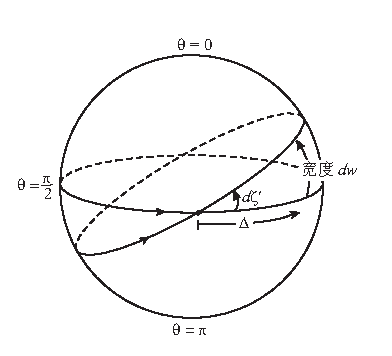
\includegraphics{../figures/chap16/fig04.eps}
}
\end{tabular}
&
\parbox{4.5cm}{\small
Figure~16.4. On a spherical Earth model the
trajectories are great circles.  Neighboring
rays cross---first at the antipodal caustic, then again
upon returning to the source, and so on.  The geometrical
spreading factor is $S=|dw|/d\zeta'=|\sin\Delta|$,
where $\Delta$
is the angular distance of propagation.}
\end{tabular}
\end{figure}
\addtocounter{figure}{1}

The unique solution to the initial-value
problem~(\ref{16.rayp3})--(\ref{16.rayp5}) on a
spherically symmetric Earth is
\eq \label{16.dynrtspher}
\p_{\zeta'}\theta(\phi)=-\sin\phi,
\qquad
\p_{\zeta'}\zeta(\phi)=\cos\phi.
\en
The geometrical spreading factor~(\ref{16.Sprac})
of a wave that has propagated a distance $\Delta$
is therefore $S=|\sin\Delta|$, as is obvious from
elementary geometrical considerations; the
caustics are degenerate points at the source
and its antipode, as illustrated in
Figure~16.4.
There is an intimate connection between these caustics
and the stationary character of the associated
ray paths: the first-arriving G1 or R1 waves are those
that have travelled along the geodesic ray path
and {\em have not\/} passed through a caustic,
whereas the later G2, G3,\hspace{0.2mm}$\ldots$ or
R2, R3,\hspace{0.2mm}$\ldots$ arrivals travel along minimax
ray paths and {\em have\/} passed through a caustic.
Roughly speaking, the Maslov index $M$ is
the number of linearly independent directions
in path space in which it is possible
to decrease rather than increase
the accumulated phase $\int_0^{\raise-.25ex\hbox{$\scriptstyle\Delta$}}
k\,d\Delta$ along a ray.  This association
between the number of caustic passages and
the character of the stationarity in Fermat's
principle is maintained in the presence of
lateral heterogeneity; in fact, it is a universal
feature of linear wave propagation in the JWKB
approximation (Gutzwiller \citeyear{gutzwiller90}).
\index{Earth model!spherical|)}%
\index{ray tracing!SNREI Earth!surface waves|)}%
\index{surface-wave ray tracing!spherical Earth|)}%

\renewcommand{\thesubsection}{$\!\!\!\raise1.3ex\hbox{$\star$}\!\!$
\arabic{chapter}.\arabic{section}.\arabic{subsection}}
\subsection{Caustic morphology}
\index{caustic!surface waves|(}%
\renewcommand{\thesubsection}{\arabic{chapter}.\arabic{section}.\arabic{subsection}}

We illustrate the nature of the surface-wave caustics
upon a laterally heterogeneous Earth by considering a
specific example: 150-second fundamental-mode Rayleigh
waves on model M84A (Woodhouse \& Dziewonski
\citeyear{woodhouse&dziewonski84}).  The
phase speed $c+\delta c$ of these waves is
a spherical-harmonic sum of maximum angular
degree $s_{\rm max}=8$, with point-to-point
variations of order $\delta c/c=\pm 2\!-\!3$~percent.
To trace surface-wave rays, we rotate the model so
that the unperturbed path lies along the equator,
and integrate equations~(\ref{16.rayp1})--(\ref{16.rayp2})
numerically using a variable-order Runge-Kutta
scheme.  Figure~\ref{fig:16.orbits}
shows a family of rays shot out at $4^\circ$ intervals from a
hypothetical source situated on the equator and Greenwich meridian
$\theta'=90^\circ$, $\phi'=0^\circ$.
The first three orbits of the rays shot toward the west
($180^\circ<\zeta'<360^\circ)$ are shown on the left and above,
whereas the first three orbits of the rays shot toward
the east ($0^\circ<\zeta'<180^\circ)$ are shown on the right
and below; the figure should be regarded as a single continuous
strip that has been cut into three panels at $\phi=\pm 400^{\circ}$
for convenience of display.
The caustics in the vicinity of the antipode and the source are evident;
half of each caustic appears on the left and above at each location,
whereas the other half appears on the right and below.
\begin{figure}[!t]
\begin{center}
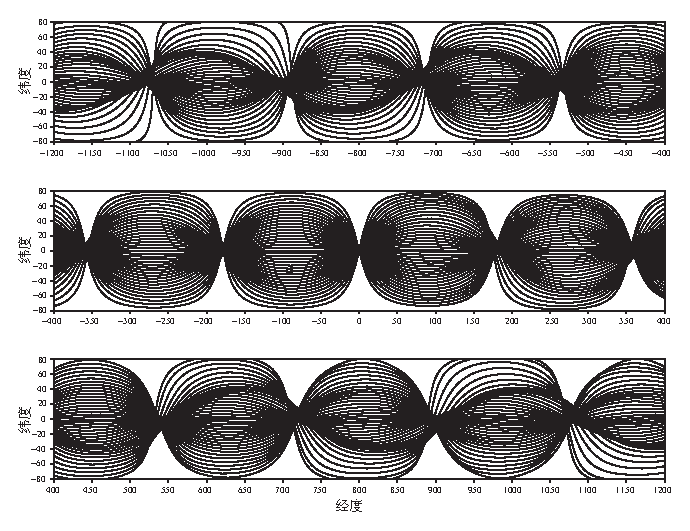
\includegraphics{../figures/chap16/fig05.eps}
\end{center}
\caption[orbits]{\label{fig:16.orbits}
Surface-wave rays shot from a
hypothetical source situated on the equator and
Greenwich meridian, in the center of the middle panel.
The phase-speed distribution is that sampled
by 150-second fundamental-mode Rayleigh waves
on Earth model M84A.  The left half of the middle
panel and the upper panel display the first three
orbits of the rays shot toward the west; the right
half of the middle panel and the lower panel display
the corresponding rays shot toward the east.  The map
is a repeating linear cylindrical projection; the right
edge of the top panel (longitude $-400^\circ$) and the
left edge of the bottom panel (longitude $400^\circ$)
coincide with the left and right edges, respectively,
of the middle panel.  Rays that pass near the North
and South Poles are not shown.}
\end{figure}

Magnified views of the central portion of
the first antipodal caustic,
where R1 and R2 interfere,
and the first source caustic,
where R2 and R3 interfere, are shown in Figure~\ref{fig:16.caustics}.
Each caustic is a single closed curve with sixteen
cusps and a continuously evolving tangent
(Wang, Dahlen \& Tromp \citeyear{wang&al93}).
The gross features of this morphology can
be understood on the basis of catastrophe theory;
surface-wave caustics are closed
curves with multiple cusps
because a fold and a cusp are
the only two structurally stable
catastrophes in two dimensions
(Poston \& Stewart \citeyear{poston&stewart78};
Berry \& Upstill \citeyear{berry&upstill80}).
Every sufficiently strong local minimum or
maximum in the surface-wave phase speed
$c+\delta c$ gives rise to a cusp;
the total number is for this
reason equal to twice the maximum
angular degree of the Earth model.
At any point that is sufficiently distant from
the source or antipode, there are only two arrivals
associated with the R1--R2 and R2--R3 caustics.
Receivers in the vicinity of the source or antipode
may have, however, four, six or more geometrical
arrivals, because of the multiplicity of the
folding. A surprisingly large fraction of the
Earth's surface area is occupied by these
complex, intricately folded caustics.
Several of the cusps of the R1--R2 and R2--R3
caustics extend out to more than
$20^{\circ}\hspace{-0.9 mm}-\!30^{\circ}$
from the antipode and source, respectively.
The R3--R4, R4--R5 and succeeding caustics are
even more extensive, because of the increasing lateral
refraction of the waves.  The divergence $S^{-1}
\rightarrow\infty$ of the geometrical spreading
factor renders the JWKB representation~(\ref{16.accsum})
of the surface-wave response invalid in the vicinity of
the source and antipodal caustics.  An alternative
Maslov representation has been
developed by Tromp \& Dahlen (\citeyear{tromp&dahlen93}).
\begin{figure}[!t]
\begin{center}
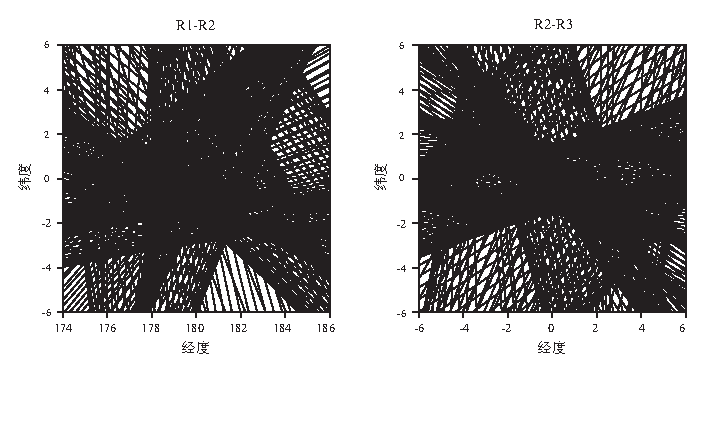
\includegraphics{../figures/chap16/fig06.eps}
\end{center}
\caption[caustics]{\label{fig:16.caustics}
Blown-up bird's-eye view of the first antipodal (R1--R2) and source
(R2--R3) caustics formed by 150-second fundamental-mode Rayleigh
waves on model M84A.  Each caustic is an envelope of the rays shot
from the source at $\theta'=\pi/2$, $\phi'=0$.  Every ray passes through
these and all succeeding caustics at a single point of tangency.}
\end{figure}
\index{caustic!surface waves|)}%

\renewcommand{\thesubsection}{$\!\!\!\raise1.3ex\hbox{$\star$}\!\!$
\arabic{chapter}.\arabic{section}.\arabic{subsection}}
\subsection{Tsunamis}
\index{tsunami|(}%
\renewcommand{\thesubsection}{\arabic{chapter}.\arabic{section}.\arabic{subsection}}

We noted in Section~8.8.11 that tsunamis, or
earthquake-generated surface gravity waves,
are the true fundamental modes of an Earth model
with a neutrally stratified fluid outer core and
surficial ocean.  As we showed in Section~11.6.3
the surface phase speed of a tsunami is very nearly that of a
shallow-water wave: $ac=\sqrt{gh}$, where $g$ is the acceleration
of gravity and $h(\theta,\phi)$ is the geographically
variable water depth.  We can use this relation
together with our knowledge of seafloor bathymetry to determine a
global tsunami phase-speed map $c(\theta,\phi)$.  Such a map was
first used to trace tsunami rays within the world's ocean basins
by Woods \& Okal (\citeyear{woods&okal87}) and Satake (\citeyear{satake88}).
In Figure~\ref{fig:16.tsunamis} we show the trajectories of
the waves generated by the great 1960 earthquake in Chile.
\index{Chile 1960 earthquake}%
Note the strong focusing and defocusing of tsunami energy
caused by the lateral variations in Pacific Ocean bathymetry.
Regions of intense focusing, such as New Zealand, Japan, Nicaragua
and Costa Rica are most likely to experience coastal
devastation associated with runup effects.

For any given coastal site, we can determine the epicentral
locations of potentially hazardous tsunamigenic earthquakes by
exploiting the principle of source-receiver reciprocity.
We consider a hypothetical tsunami source at the site itself,
and trace rays to the periphery of the adjacent or surrounding
ocean basin, as illustrated for the island of
Tahiti in Figure~\ref{fig:16.tsunami_rec}.  Those active seismic
regions that exhibit strong ``reciprocal focusing'' are the most
likely birthplaces of tsunamis that could affect the site in question.
Tahiti, for example, is seen to be particularly susceptible to
tsunamis generated by earthquakes in the Philippine and Kuril
Islands and along selected regions of the South American coast.
This {\em reciprocal map\/}
\index{reciprocal map}%
technique was introduced by Woods \& Okal (\citeyear{woods&okal87}).
\begin{figure}
\begin{center}
\scalebox{0.85}{
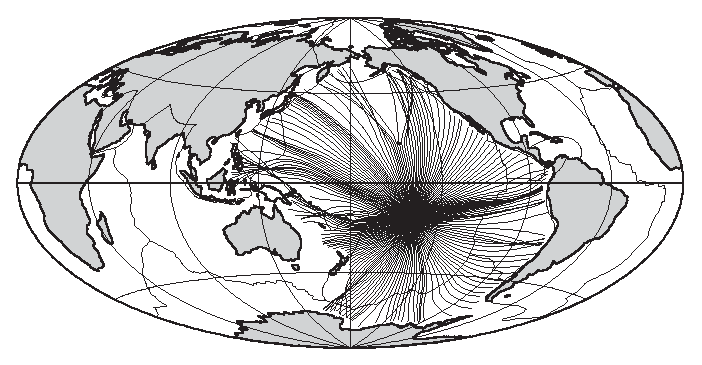
\includegraphics{../figures/chap16/fig08.eps}
}
\end{center}
\caption[tsunamis]{\label{fig:16.tsunamis}
Tsunami trajectories shot at equally spaced takeoff-angle
increments from the epicenter of the 1960 Chile earthquake.}
\end{figure}

As a tsunami propagates, its local eigenfunctions $U$ and $V$
adiabatically adjust to the variations in water depth $h$,
stretching vertically to fill the deep ocean where the wave
travels rapidly, and compressing and increasing in amplitude
over a shallower shelf, plateau or spreading ridge where the
wave slows down.  We illustrate these variations in the local
radial structure of the tsunami mode along a cross-section
of the South Pacific in Figure~\ref{fig:16.tsunami_locmod}.
\begin{figure}[!t]
\begin{center}
\scalebox{0.85}{
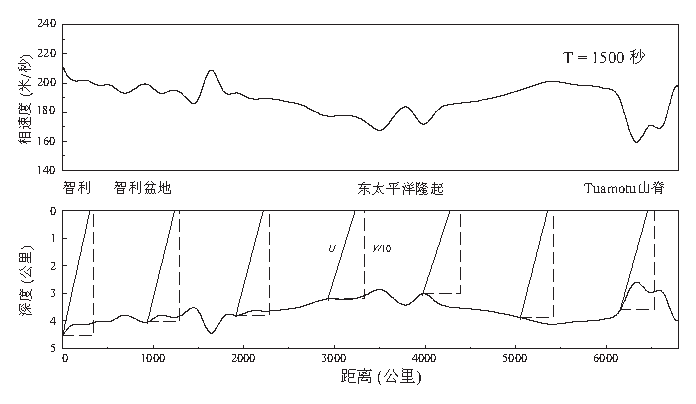
\includegraphics{../figures/chap16/fig09.eps}
}
\end{center}
\caption[tsunami_rec]{\label{fig:16.tsunami_rec}
Trajectories of tsunamis generated by a fictitious earthquake
on the island of Tahiti.  Rays are shot at equally spaced
takeoff-angle increments; the seismic reciprocity principle
may be used to identify potentially dangerous tsunamigenic
source regions along the Pacific rim.
}
\end{figure}
\begin{figure}[!b]
\begin{center}
\scalebox{0.85}{
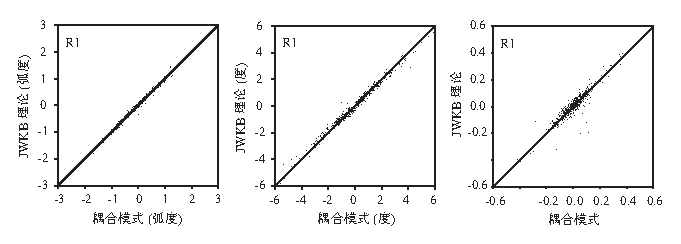
\includegraphics{../figures/chap16/fig10.eps}
}
\end{center}
\caption[tsunami_locmod]{\label{fig:16.tsunami_locmod}
({\em Top\/}) Shallow-water gravity-wave speed $ac=\sqrt{gh}$
along a 6500~km cross-section extending from Chile
to the Tuamoto Ridge across the East Pacific Rise.
({\em Bottom\/}) Variation of the local tsunami
eigenfunctions $U$ ({\em solid line\/}) and $V/10$
({\em dashed line\/}) along the same cross-section.
The local modes adiabatically adapt themselves to the
slowly varying bathymetry $h$; the tangential displacement
is very nearly uniform throughout the water column.  The
quantities plotted are the JWKB-normalized ($c\hspace{0.2 mm}CI_1=1$)
displacements for a $2\pi/\omega=1500$~s tsunami.
}
\end{figure}
As noted in Section~8.8.11, the displacement is predominantly horizontal;
note that $V/10$ is plotted rather than $V$.  The open-ocean height of a
tsunami is determined by both variations in ray-tube width due to lateral
refraction and the shallow-water amplification effect depicted here.
Local harbor geometry and bathymetry govern its ultimate fate during
the non-linear runup phase, once it reaches the shore.
\index{tsunami|)}%

\renewcommand{\thesection}{$\!\!\!\raise1.3ex\hbox{$\star$}\!\!$
\arabic{chapter}.\arabic{section}}
\section{Validity of JWKB Theory}
\index{JWKB theory!validity of|(}%
\renewcommand{\thesection}{\arabic{chapter}.\arabic{section}}

Surface-wave JWKB theory is a useful means of computing
synthetic long-period seismograms, because of its
physical simplicity and numerical efficiency.
Like other ray-based methods, however, its
applicability is subject to severe restrictions.
First, as we have seen, it is invalid
in the vicinity of the source and antipodal
caustics, where neighboring rays cross.
Second, even away from caustics, JWKB theory
is valid only in the limit of a {\em smooth\/}
lateral heterogeneity.  The requirement that the
angular wavelength $\lambda =2\pi k^{-1}$ of the wave must be
small compared to the characteristic angular scale
$\Lambda_{\Omega}$ of the heterogeneity is necessary but not
sufficient.  A necessary and sufficient condition
is that the perturbation in phase speed must not change
appreciably across the width of the {\em first Fresnel
zone\/} surrounding a surface-wave trajectory;
\index{Fresnel zone}%
this zone is the locus of single-scattering
points $\brh''$
for which (Kravtsov \& Orlov \citeyear{kravtsov&orlov90})
\eq \label{16.Fresnel1}
|\psi(\brh'',\brh')+\psi(\brh,\brh'')
-\psi(\brh,\brh')|\leq\pi,
\en
where $\psi(\brh'',\brh')=\int_{\hat{\mbox{\scriptsize\bf r}}'}
^{\hat{\mbox{\scriptsize\bf r}}''}\bk\cdot d\brh$,
$\psi(\brh,\brh'')=\int_{\hat{\mbox{\scriptsize\bf r}}''}
^{\hat{\mbox{\scriptsize\bf r}}}\bk\cdot d\brh$
and $\psi(\brh,\brh')=\int_{\hat{\mbox{\scriptsize\bf r}}'}
^{\hat{\mbox{\scriptsize\bf r}}}\bk\cdot d\brh$ are the
phases accumulated along the source-scatterer,
scatterer-receiver and source-receiver ray paths, respectively.
The angular width of a surface-wave Fresnel zone
at a typical scattering point
midway between the source and receiver on a
slightly heterogeneous Earth is $\delta\approx\sqrt{\lambda/2}$;
a simple heuristic condition for the validity of surface-wave
JWKB theory away from caustics is therefore
(Wang \& Dahlen \citeyear{wang&dahlen95})
\eq \label{16.Fresnel2}
\sqrt{\lambda/2\Lambda_{\Omega}^2}\ll 1.
\en
Because of the spherical geometry, the Fresnel-zone
width $\delta\rightarrow 0$ at both the source-to-receiver
and receiver-to-source caustics, rather than growing
indefinitely as the number of orbits increases;
for this reason, the restriction~(\ref{16.Fresnel2})
is applicable to G2, G3,\hspace{0.2mm}$\ldots$ and R2, R3,\hspace{0.2mm}$\ldots$
waves as well as to the minor-arc arrivals G1 and R1.

The validity of surface-wave JWKB theory can also be assessed
by comparing its predictions against more accurate coupled-mode
calculations.  Love-to-Rayleigh scattering and scattering
between one Love or Rayleigh mode branch and another are
neglected in the along-branch coupling scheme described in
Section~14.3.7; however, diffraction and other finite-frequency
wave-propagation effects that are
ignored in JWKB theory are fully accounted for.
In Figure~\ref{fig:16.JWKB_CM}, we present a comparison between
\begin{figure}[!b]
\begin{center}
\scalebox{1.0}{
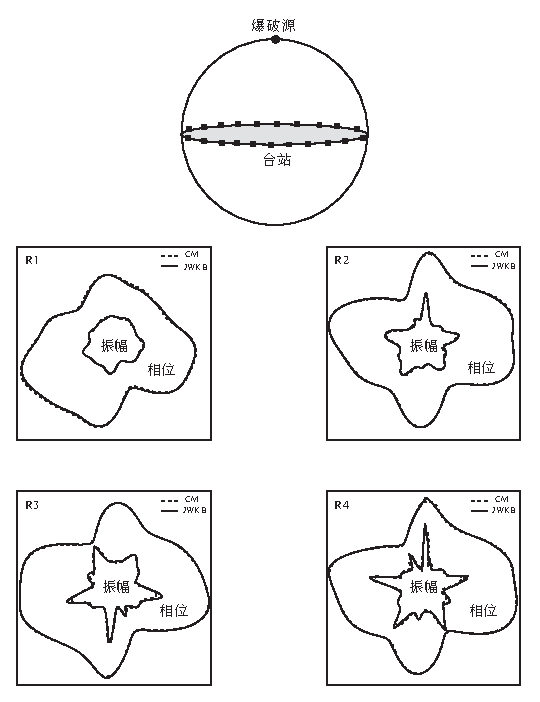
\includegraphics{../figures/chap16/fig11.eps}
}
\end{center}
\caption[JWKB_CM]{\label{fig:16.JWKB_CM}
Comparison of JWKB observables with those measured
by processing synthetic coupled-mode accelerograms
on model S12WM13 of Su, Woodward \& Dziewonski
(\citeyear{su&al94}).  All results are for 150-second
R1 Rayleigh waves in the epicentral distance range
$60^\circ<\Theta<120^\circ$; each dot represents
one minor-arc path.  ({\em Left\/}) Phase anomalies
$\psi-\psi_{\rm spher\,\oplus}$, measured in radians.
({\em Middle\/}) Azimuthal arrival-angle anomalies
$\zeta-\zeta_{\rm spher\,\oplus}$, measured in degrees,
counterclockwise from due south at the receiver.
({\em Right\/}) Dimensionless (fractional) amplitude anomalies
$(A-A_{\rm spher\,\oplus})/A_{\rm spher\,\oplus}$.}
\end{figure}
the JWKB phase, arrival-angle and amplitude anomalies on model
S12WM13 with the corresponding results obtained by processing
synthetic single-branch accelerograms.  All comparisons are carried
out for 150-second fundamental-mode Rayleigh waves recorded on
the radial component at fifty GSN station locations following
twenty earthquakes that occurred between 1977 and 1984---a total
of 1000 source-receiver paths.
The accelerograms $a(t)$ are calculated using the real
symmetric variational method, with each target multiplet along
the ${}_0{\rm S}_l$ branch coupled to its nearest $\pm5$ neighbors.
The phase and amplitude anomalies $\psi-\psi_{\rm spher\,\oplus}$ and
$(A-A_{\rm spher\,\oplus})/A_{\rm spher\,\oplus}$
are measured by cross-correlation
with the corresponding spherical-Earth accelerograms
$a_{\rm spher\,\oplus}(t)$, using a one-hour time window centered upon the
arrival of the R1 wavetrain at the period of interest.
The arrival-angle anomalies $\zeta-\zeta_{\rm spher\,\oplus}$
are measured using a simple algorithm that minimizes the
power on the transverse component; the north-south and
east-west components are rotated to new components oriented
at $\pm45^{\circ}$ to the unperturbed ray-arrival direction
prior to processing, to reduce numerical errors.
To avoid the overlapping of neighboring wavetrains at
the source and antipodal caustics, we only consider paths
with source-receiver distances in the range $60^\circ<\Theta<120^\circ$;
\begin{figure}[!t]
\begin{center}
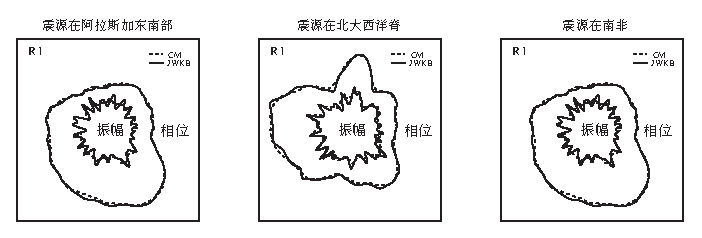
\includegraphics{../figures/chap16/fig12.eps}
\end{center}
\caption[JWKB_CM_ring1]{\label{fig:16.JWKB_CM_ring1}
Polar plot of the phase anomaly $\psi-\psi_{\rm spher\,\oplus}$
({\em outer curve\/}) and amplitude anomaly
$A-A_{\rm spher\,\oplus}$ ({\em inner curve\/}) of
150-second R1--R4 Rayleigh waves at an epicentral
distance of $\Theta=90^\circ$ away from an explosive
source located near the coast of Peru on model S12WM13.
The outer curves are effectively a snapshot of a
150-second wavefront, whereas the inner curves show
the variation of the amplitude along this wavefront.
Cartoon ({\em top\/}) depicts the source-receiver
geometry.  The abbreviation CM stands for coupled-mode.}
\end{figure}
we also discard a small number of paths having small
unperturbed amplitudes compared with those
at other stations for the same earthquake;
these seismograms correspond to waves leaving the
source near the nodes of the surface-wave radiation pattern.
The final dataset consists of slightly more than
500 minor-arc paths.  In general, the JWKB
results are in good agreement with the coupled-mode
measurements on model S12WM13, which has $s_{\rm max}=12$
and $\Lambda_{\Omega}\approx 60^{\circ}$.
The phase-anomaly predictions $\psi-\psi_{\rm spher\,\oplus}$ are
more accurate than the arrival-angle predictions
$\zeta-\zeta_{\rm spher\,\oplus}$, and these in turn are
more accurate than the amplitude-anomaly predictions
$(A-A_{\rm spher\,\oplus})/A_{\rm spher\,\oplus}$.  This is an expected
feature of the approximation on a slightly heterogeneous
Earth, as we shall see in Section~\ref{16.sec.raypert}.
The first-order phase, arrival-angle and amplitude
perturbations $\delta\psi$, $\delta\zeta$ and $\delta A/A$
depend upon the zeroth, first and second cross-path
derivatives of the phase-speed anomaly, respectively;
thus, in a sense, each of these observables ``sees''
an increasingly ``rough'' image of the Earth.\vspace{-0.5mm}

\begin{figure}[!b]
\begin{center}
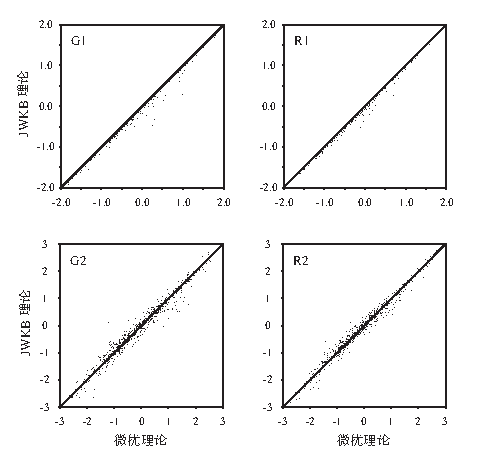
\includegraphics{../figures/chap16/fig13.eps}
\end{center}
\caption[JWKB_CM_ring2]{\label{fig:16.JWKB_CM_ring2}
Same as Figure~\protect\ref{fig:16.JWKB_CM_ring1}
for three explosive sources located in southeastern Alaska,
on the North Atlantic Ridge and in South Africa, on a
moderately roughened version of model S12WM13.
The 150-second R1 waves have propagated an unperturbed
epicentral distance $\Theta=90^{\circ}$.  Finite-frequency
diffraction effects have a tendency to smooth out
ray-theoretical ``crinkles'' in the shape
and---particularly---the amplitude of a wavefront.}
\end{figure}
There is a tendency for JWKB theory to
overestimate absolute phase and amplitude anomalies
$|\psi-\psi_{\rm spher\,\oplus}|$ and
$|A-A_{\rm spher\,\oplus}|/A_{\rm spher\,\oplus}$.
This bias is due to a finite-frequency {\em wavefront smoothing\/}
\index{wavefront smoothing}%
phenomenon---diffraction acts to smooth out irregularities
that would be present in the infinite-frequency
wavefronts that are governed by ray theory.
To illustrate this effect, we describe the results of a
simple numerical experiment: a ring of
receivers is deployed at an epicentral
distance $\Theta=90^\circ$ away from a hypothetical
explosive source, with an isotropic moment tensor $\bM=M_0\bI$.
The use of an isotropic source serves to eliminate radiation-pattern
effects.   Figure~\ref{fig:16.JWKB_CM_ring1} compares the JWKB and
coupled-mode phase and amplitude anomalies of 150-second
fundamental-mode R1--R4 Rayleigh waves on model S12WM13,
due to an explosion located near the coast of Peru; note
that JWKB theory predicts the phase and amplitude of the
radiated wavefield quite accurately.
To investigate the
effect of rougher lateral variation on surface-wave propagation,
we contrive a ``model'' with maximum angular degree
$s_{\rm max}=36$  and $\Lambda_{\Omega}\approx 45^{\circ}$ by
adding pseudo-random higher-degree structure to model S12WM13;
the added power accounts for less than 10\% of the total
perturbation in the phase speed $\delta c$ of a 150-second
Rayleigh wave. Figure~\ref{fig:16.JWKB_CM_ring2} shows a
comparison of the Rayleigh waves generated by three explosions
located in southeastern Alaska, on the North Atlantic
Ridge and in South Africa, on this slightly rougher
version of model S12WM13.  The agreement between the
JWKB and coupled-mode phase anomalies is not as good
as for the R1 waves in Figure~\ref{fig:16.JWKB_CM_ring1};
both discrepancies are consistent with the heuristic validity
criterion~(\ref{16.Fresnel2}).  The wavefront smoothing
effect is particularly pronounced in this example for the
amplitude anomaly $A-A_{\rm spher\,\oplus}$.  On even rougher models,
the JWKB phase anomaly $\psi-\psi_{\rm spher\,\oplus}$ would appear to be
similarly ``crinkled'' compared to the true finite-frequency phase.
\index{JWKB theory!validity of|)}%

\section{Ray Perturbation Theory}
\index{ray perturbation theory!surface waves|(}%
\index{surface-wave perturbation theory|(}%
\index{perturbation!surface waves|(}%
\label{16.sec.raypert}

Suppose now that the lateral heterogeneity of the Earth
is {\em slight as well as smooth\/}, so that the phase
speed of a Love or Rayleigh wave can be treated as a
\index{perturbation!smooth}%
\index{perturbation!slight}%
first-order perturbation away from the uniform speed
upon a spherically symmetric Earth:
\eq \label{16.raypert1}
c\rightarrow c+\delta c \quad\mbox{where}\quad |\delta c|\ll c.
\en
The rays upon such an Earth model will deviate slightly
from the great-circular rays upon a spherically symmetric
Earth; as a result, the amplitude and phase of a surface
wave will be perturbed:
\eq
A\rightarrow A+\delta A,\qquad
\psi\rightarrow\psi+\delta\psi,
\en
where
\eq \label{16.dA}
\frac{\delta A}{A}=\frac{\delta A_{\rm r}}{A_{\rm r}}
+\frac{\delta A_{\rm p}}{A_{\rm p}}
+\frac{\delta A_{\rm s}}{A_{\rm s}},
\en
\eq \label{16.dpsi}
\delta\psi=\delta\psi_{\rm r}+\delta\psi_{\rm p}
+\delta\psi_{\rm s}.
\en
The subscripts ${\rm s}$, ${\rm p}$ and ${\rm r}$
identify the terms associated with the source, path
and receiver, respectively.  A surface-wave analogue of
the {\em ray perturbation theory\/} developed in Section~\ref{section:15.9}
can be used to find the geometry of the perturbed rays,
as well as the first-order amplitude and phase perturbations
$\delta A_{\rm s}/A_{\rm s}$, $\delta A_{\rm p}/A_{\rm p}$,
$\delta A_{\rm r}/A_{\rm r}$ and $\delta\psi_{\rm s}$,
$\delta\psi_{\rm p}$, $\delta\psi_{\rm r}$.  We follow
our usual custom, and employ a prime and a subscript s
interchangeably to identify quantities such as
$\zeta'=\zeta_{\rm s}$ evaluated at the source.

\subsection{Fermat phase}
\index{Fermat phase|(}%

As in the body-wave case, Fermat's principle enables us to
determine the first-order perturbation in the accumulated
phase between the source and receiver by integration
along the {\em unperturbed great-circular ray path\/}:
\eq \label{16.dpsip}
\delta\psi_{\rm p}=\int_0^\Delta\delta k\,d\phi
=-\om c^{-2}\int_0^\Delta\delta c\,d\phi,
\en
\begin{figure}[!b]
\begin{center}
\scalebox{1.1}{
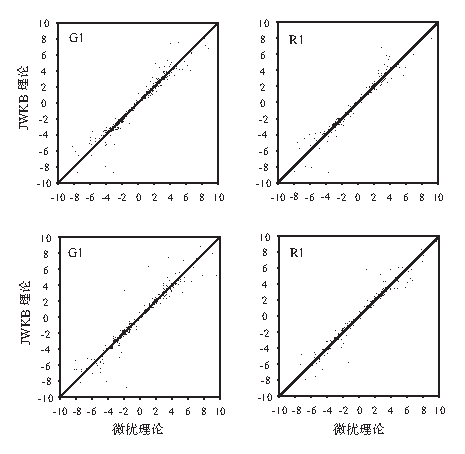
\includegraphics{../figures/chap16/fig14.eps}
}
\end{center}
\caption[phase]{\label{fig:16.phase}
Scatter-plot comparison of the first-order path
phase anomaly $\psi_{\rm p}$ with the exact JWKB phase
anomaly $\psi_{\rm p}-\psi_{\rm p}^{\rm spher\,\oplus}$
for 165-second fundamental-mode surface waves on model S12WM13.
Each of the 850 points represents a single G1, R1, G2 or R2 path.
The phase anomalies are plotted in radians. There is an obvious
Fermat bias for the first-arriving G1 and R1 waves ({\em top\/}),
but none for the later G2 and R2 arrivals that have passed through
an antipodal caustic ({\em bottom\/}).}
\end{figure}
where the source and receiver are presumed to be situated
on the equator, as before.  The result~(\ref{16.dpsip})
is valid for all G1, G2,\hspace{0.2mm}$\ldots$ and R1, R2,\hspace{0.2mm}$\ldots$ waves;
the integration is over the full ray path of length $\Theta,
2\pi-\Theta,\ldots$ in the case of a multi-orbit wave.
Figure~\ref{fig:16.phase} compares the first-order
Fermat phase delays $\delta\psi_{\rm p}$ of a
number of first-arriving and second-arriving Love and
Rayleigh waves with the exact or true-path phase delays
$\psi_{\rm p}-\psi_{\rm p}^{\rm spher\,\subearth}$
calculated by means of two-point ray tracing.
The exact delays of all G1 and R1 waves
are always less than the approximate Fermat delays,
\eq
\psi_{\rm p}-\psi_{\rm p}^{\rm spher\,\subearth}<
\delta\psi_{\rm p},
\en
in accordance with the variational principle---the true
ray path followed
by a minor-arc wave is the minimum-phase path.
The stationary ray paths of G2, R2 and other
higher-orbit waves are not minimum-phase; there is thus
no such {\em Fermat bias\/} for these minimax arrivals.
\index{Fermat bias}%
\index{Fermat phase|)}%

\subsection{Fictitious frequency and source shift}
\index{fictitious frequency shift|(}%
\index{fictitious source shift|(}%
\label{16.sec.WDGC}

In the so-called {\em path-average\/} or
{\em great-circle approximation\/} to the
\index{path-average approximation}%
\index{great-circle approximation}%
moment-tensor response~(\ref{16.TDneed1})--(\ref{16.TDneed2}),
the perturbation to the spherical-Earth
amplitude $A=A_{\rm r}A_{\rm p}A_{\rm s}$
is ignored, and only the path contribution~(\ref{16.dpsip})
to the first-order perturbation in the phase
$\psi_{\rm r}+\psi_{\rm p}+\psi_{\rm s}$
is accounted for:
\eq
\delta A=0,\qquad\delta\psi=\delta\psi_{\rm p}.
\en
We can rewrite the first-order phase delay~(\ref{16.dpsip})
for the odd-arriving and even-arriving waves in terms of the
minor-arc and full great-circular averages of $\delta k$ in the form
\eq \label{16.WD1}
\delta\psi=\left\{\begin{array}{ll}
\delta\hat{k}\,\Theta+\delta\bar{k}\,(s-1)\pi,
& \hspace{4.0 mm}\mbox{$s$ odd} \\
\vspace{-1.0 mm} & \vspace{-1.0 mm} \\
\delta\bar{k}\,s\pi-\delta\hat{k}\,\Theta,
& \hspace{4.0 mm}\mbox{$s$ even},
\end{array}\right.
\en
where
\eq \label{16.WD2}
\delta\hat{k}=\frac{1}{\Theta}\int_0^{\Theta}
\delta k\,d\phi,\qquad
\delta\bar{k}=\frac{1}{2\pi}\oint
\delta k\,d\phi.
\en
This travelling-wave phase shift may alternatively be expressed
in terms of a fictitious perturbation in the wavenumber
$\delta\bar{k}$ and epicentral distance $\delta\Theta$
{\em upon a spherical Earth\/} in the form
\eq \label{16.WD3}
\delta\psi=\left\{\begin{array}{ll}
\delta\bar{k}\,\Delta+k\,\delta\Theta,
& \hspace{4.0 mm}\mbox{$s$ odd} \\
\vspace{-1.0 mm} & \vspace{-1.0 mm} \\
\delta\bar{k}\,\Delta-k\,\delta\Theta,
& \hspace{4.0 mm}\mbox{$s$ even}.
\end{array}\right.
\en
Upon equating~(\ref{16.WD1}) and~(\ref{16.WD3}) we deduce that
\eq \label{16.WD4}
\frac{\delta\Theta}{\Theta}=-\frac{\delta\hat{k}
-\delta\bar{k}}{k}=\frac{\delta\hat{c}
-\delta\bar{c}}{c}=\frac{c}{C}\frac{\delta\hat{\omega}
-\delta\bar{\omega}}{\omega}.
\en
The quantities $\delta\hat{\omega}$ and $\delta\bar{\omega}$
are the minor-arc and great-circular averages of the local
perturbation $\delta\om$ in the eigenfrequency of the
associated normal mode or standing wave:
\eq \label{16.WD5}
\delta\hat{\omega}=\frac{1}{\Theta}\int_0^{\Theta}
\delta\omega\,d\phi,\qquad
\delta\bar{\omega}=\frac{1}{2\pi}\oint
\delta\omega\,d\phi.
\en
These results enable us to calculate an approximate
synthetic accelerogram upon a laterally heterogeneous
Earth by means of a modest modification to the mode-summation
procedure employed upon a spherically symmetric Earth
(Woodhouse \& Dziewonski \citeyear{woodhouse&dziewonski84}).
It is simply necessary to replace the eigenfrequency
$\om$ of each mode and the epicentral distance $\Theta$
in equations~(\ref{10.DISPUGLY})--(\ref{10.Dexpl2}) by
$\om+\delta\bar{\omega}$ and $\Theta+\delta\Theta$,
respectively.  Note that this must be done on both a
mode-by-mode and a path-by-path basis; nevertheless,
the method is extremely efficient, requiring very little
more time than the corresponding summation on a spherical Earth.
Even though the fictitious source shift~(\ref{16.WD4}) is
determined by requiring that the first-order phase
perturbations~(\ref{16.WD1}) and~(\ref{16.WD3})
must match for all possible orbits, the great-circle
approximation is fundamentally a {\em short-time
approximation\/}, because of the tendency of the
higher-orbit ray paths to diverge farther and
farther from the unperturbed great-circle
(see Sections~14.3.7 and~16.8.4).
\index{fictitious frequency shift|)}%
\index{fictitious source shift|)}%

\renewcommand{\thesubsection}{$\!\!\!\raise1.3ex\hbox{$\star$}\!\!$
\arabic{chapter}.\arabic{section}.\arabic{subsection}}
\subsection{Ellipticity correction}
\index{ellipticity correction!surface waves|(}%
\renewcommand{\thesubsection}{\arabic{chapter}.\arabic{section}.\arabic{subsection}}

We demonstrated in Section~\ref{section:rotell}
that the combined effect of the Earth's hydrostatic
ellipticity $\eps$ and aspherical centrifugal potential
$\psi-\bar{\psi}$ upon an isolated normal-mode multiplet
is governed by a diagonal $(2l+1)\times (2l+1)$ splitting
matrix of the form
\eq \label{16.ellcorr1}
H_{mm'}^{\rm ell}=\om a^{\rm ell}(1-3m^2\hspace{-0.3 mm}/k^2)\,\delta_{mm'},
\en
where $\om$ is the unperturbed eigenfrequency and $k=\sqrt{l(l+1)}$.
The quantity $a^{\rm ell}$ is the dimensionless ellipticity
splitting parameter, given by
\eqa \label{16.ellsplit} \lefteqn{
a^{\rm ell}=\frac{l(l+1)}{2(2l+3)(2l-1)\om^2}} \nonumber \\
&&\mbox{}\times\int_0^a\twothirds\eps\Bigl\{
\kappa\bigl[\bar{V}_\kappa
-(\eta+1)\check{V}_\kappa\bigr]
+\mu\bigl[\bar{V}_\mu
-(\eta+1)\check{V}_\mu\bigr] \nonumber \\
&&\mbox{}\qquad
+\rho\bigl[(\bar{V}_\rho-\om^2\bar{T}_\rho)
-(\eta+3)(\check{V}_\rho-\om^2\check{T}_\rho\bigr]\Bigr\}r^2dr,
\ena
where $\eta=r\dot{\eps}/\eps$, and $\bar{V}_\kappa$,
$\check{V}_\kappa$, $\bar{V}_\mu$, $\check{V}_\mu$
and $\bar{V}-\om^2\bar{T}_\rho$, $\check{V}_\rho-\om^2\check{T}_\rho$ 
are the elliptical incompressibility, rigidity and density kernels
defined in equations (\ref{D.selffirst})--(\ref{D.selflast}).
In the present context, it is more convenient to regard the ellipticity as
a degree-two zonal perturbation to either the local eigenfrequency $\om$
of an $n=0,1,2,\ldots$ toroidal or spheroidal mode or the phase speed
$c$ of the equivalent Love or Rayleigh wave:
\eq \label{16.ellcorr2}
\delta\om^{\rm ell}=\delta\om_{20}^{\rm ell}X_{20}(\theta),\qquad
\delta c^{\rm ell}=\delta c_{20}^{\rm ell}X_{20}(\theta),
\en
where $X_{20}(\theta)=\fourth\sqrt{5/\pi}\,(3\cos^2\theta-1)$ and
$\delta c_{20}^{\rm ell}/c=(c/C)(\delta\om_{20}^{\rm ell}/\om)$
as usual.  We can relate the coefficients in~(\ref{16.ellcorr2})
to the ellipticity splitting parameter~(\ref{16.ellsplit}) by
making use of the asymptotic representation~(\ref{14.Lambdapp2})
of the splitting matrix~(\ref{16.ellcorr1}):
\eq \label{16.ellcorr3}
H_{mm'}^{\rm ell}\approx\eighth\sqrt{5/\pi}\,\delta\om_{20}^{\rm ell}
\,(1-3m^2\hspace{-0.3 mm}/k^2)\,\delta_{mm'}.
\en
This approximation is valid provided that $k\gg 1$.
Upon comparing~(\ref{16.ellcorr1}) and~(\ref{16.ellcorr3})
we find that
\eq \label{16.ellcorr4}
\delta\om_{20}^{\rm ell}=4\sqrt{4\pi/5}\,\om a^{\rm ell},\qquad
\delta c_{20}^{\rm ell}=4\sqrt{4\pi/5}\,(c^2\hspace{-0.3 mm}/C) a^{\rm ell}.
\en
Prior to computing synthetic JWKB accelerograms~(\ref{16.accsum})
on a hydrostatic elliptical, laterally heterogeneous Earth, it is necessary
to convert the event and station locations from geographic to
geocentric coordinates as discussed in Section~\ref{section:14.geocen},
in addition to accounting for the degree-two zonal contribution
$\delta c^{\rm ell}=4\sqrt{4\pi/5}\,
(c^2\hspace{-0.3 mm}/C) a^{\rm ell}X_{20}(\theta)$
to the surface-wave phase speed.
Ellipticity can be accounted for in the Woodhouse-Dziewonski
great-circle approximation by adding terms
\eq \label{16.ellcorr5}
\delta\bar{\om}^{\rm ell}=\om a^{\rm ell}(1-3\cos^2\bar{\theta}),
\en
\eq \label{16.ellcorr6}
\delta\Theta^{\rm ell}=-3(c/C)a^{\rm ell}\sin\Theta
\sin^2\bar{\theta}\cos2\phi_{\rm mp}
\en
to the fictitious frequency and source shift of each
spherical-Earth mode.  Equation~(\ref{16.ellcorr6}) is the
result of substituting the perturbation~(\ref{16.ellcorr2})
into~(\ref{16.WD4}); the angle $\phi_{\rm mp}$ is the
azimuth, measured counterclockwise from due south,
of the midpoint of the minor arc from the pole
$\bar{\theta},\bar{\phi}$ of the source-receiver
great circle.
\index{ellipticity correction!surface waves|)}%

\renewcommand{\thesubsection}{$\!\!\!\raise1.3ex\hbox{$\star$}\!\!$
\arabic{chapter}.\arabic{section}.\arabic{subsection}}
\subsection{Ray geometry}
\index{ray geometry!surface-wave|(}%
\renewcommand{\thesubsection}{\arabic{chapter}.\arabic{section}.\arabic{subsection}}

To determine the perturbation in the geometry of a
G1 or R1 surface-wave trajectory, we make the following
substitutions in the kinematic ray-tracing
equations~(\ref{16.rayp1}) and~(\ref{16.rayp2}):
\eq \label{16.raypoot1}
\theta\rightarrow\pi/2+\delta\theta,
\qquad
\zeta\rightarrow\pi/2+\delta\zeta.
\en
The source and receiver are assumed to be situated on the
equator at longitudes $\phi=0$ and $\phi=\Theta$, respectively,
so that the unperturbed ray path is given by~(\ref{16.spherray}).
Correct to first order in the small perturbations $\delta\theta$
and $\delta\zeta$, we obtain a system of linear equations governing
the perturbed ray:
\eq
\frac{d}{d\phi}\delta\theta=-\delta\zeta,\qquad
\frac{d}{d\phi}\delta\zeta=\delta\theta+c^{-1}\p_\theta\delta c.
\label{16.pray1}
\en
Equations~(\ref{16.pray1}) may be rewritten using
a $2\times 2$ matrix notation analogous to~(\ref{15.LT7vector}):
\eq
\frac{d\ssy}{d\phi}=\ssA\ssy+\ssf,
\label{16.vector}
\en
where
\eq \label{16.matrixA}
\ssy=\left(\begin{array}{c}
\delta\theta \\
\vspace{-2.0 mm} \\
\delta\zeta
\end{array}\right),
\qquad
\ssf=\left(\begin{array}{c}
0 \\
\vspace{-2.0 mm} \\
c^{-1}\delta c
\end{array}\right),
\qquad
\ssA=\left(\begin{array}{lr}
0 & -1 \\
\vspace{-2.0 mm} & \\
1 & 0
\end{array}\right).
\en
The coefficient matrix $\ssA$ is identical,
and so therefore is the propagator:
\eq\label{16.prop}
\ssP(\phi,\tilde{\phi})=\left(\begin{array}{lr}
\cos(\phi-\tilde{\phi}) & -\sin(\phi-\tilde{\phi}) \\
\vspace{-2.0 mm} & \\
\sin(\phi-\tilde{\phi}) & \cos(\phi-\tilde{\phi})
\end{array}\right).
\en
The solution to~(\ref{16.vector}) can be written in terms
of the propagator~(\ref{16.prop}) in the form~(\ref{15.LT7solution2}):
\eq \label{16.solution}
\ssy(\phi)=\int_0^{\phi}\ssP(\phi,\tilde{\phi})
\hspace{0.4 mm}\ssf(\tilde{\phi})\,d\tilde{\phi}
+\ssP(\phi,0)\hspace{0.4 mm}\ssy(0).
\en
The endpoint conditions stipulate that the perturbed ray must emanate
from the same source and hit the same receiver as the unperturbed ray:
\eq \label{16.bc}
\ssy(0)=
\left(\begin{array}{c}
0 \\
\vspace{-2.0 mm} \\
\delta\zeta'
\end{array}\right),
\qquad
\ssy(\Theta)=
\left(\begin{array}{c}
0 \\
\vspace{-2.0 mm} \\
\delta\zeta
\end{array}\right),
\en
where $\delta\zeta'$ and $\delta\zeta$ denote the
perturbed takeoff and arrival angles, respectively.
Upon inserting~(\ref{16.bc}) into~(\ref{16.solution})
we find that
\eq \label{16.takeoff}
\delta\zeta'=-(c\sin\Theta)^{-1}\int_0^\Theta\sin(\Theta-\phi)
\,\p_\theta\delta c\,d\phi,
\en
\eq \label{16.arrival}
\delta\zeta=(c\sin\Theta)^{-1}\int_0^\Theta\sin\phi
\,\p_\theta\delta c\,d\phi.
\en
Equations~(\ref{16.takeoff}) and~(\ref{16.arrival}) are the
surface-wave analogues of~(\ref{15.LT7takeoff1}) and~(\ref{15.LT7arrival1}).
An interchange $\phi\longleftrightarrow\Theta-\phi$ of the source
and receiver interchanges the angles
$\delta\zeta\longleftrightarrow\delta\zeta'$,
as expected.
The complete solution at intermediate points $0\leq\phi\leq\Theta$
analogous to~(\ref{15.LT7p1}) and~(\ref{15.LT7p2}) is
\eq \label{16.pert1}
\delta\hspace{-0.1 mm}\theta(\phi)=-c^{-1}\int_0^\phi\sin(\phi-\tilde{\phi})
\,\p_\theta\delta\tilde{c}\,d\tilde{\phi}-\delta\zeta'\sin\phi,
\en
\eq \label{16.pert2}
\delta\zeta(\phi)=c^{-1}\int_0^\phi\cos(\phi-\tilde{\phi})
\,\p_\theta\delta\tilde{c}\,d\tilde{\phi}+\delta\zeta'\cos\phi,
\en
where the tildes denote evaluation at the dummy integration
variable $\tilde{\phi}$.
Note that $\delta\hspace{-0.1 mm}\theta(0)=\delta\theta(\Theta)=0$
whereas $\delta\zeta(0)=\delta\zeta'$ and $\delta\zeta(\Theta)=
\delta\zeta$, as expected.  The first-order takeoff-angle
\index{shooting!initial guess}%
\begin{figure}[!b]
\begin{center}
\scalebox{1.1}{
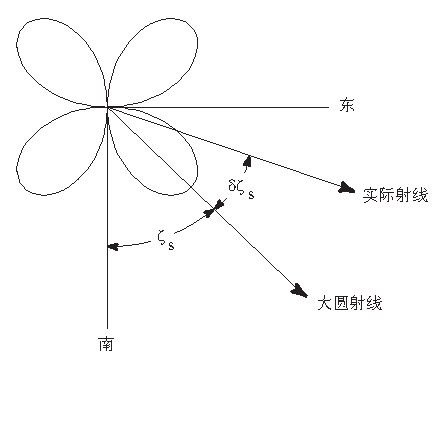
\includegraphics{../figures/chap16/fig15.eps}
}
\end{center}
\caption[takeoff]{\label{fig:16.takeoff}
Scatter-plot comparison of the first-order azimuthal
anomalies with the exact JWKB deflections suffered by
165-second fundamental-mode surface waves on
model S12WM13.  ({\em Top\/}) Takeoff-angle
anomalies $\delta\zeta'$ versus
$\zeta'-\zeta^{\prime}_{\rm spher\,\oplus}$.
({\em Bottom\/}) Arrival-angle anomalies
$\delta\zeta$ versus $\zeta-\zeta_{\rm spher\,\oplus}$.
Each of the 850 points represents a single G1 or R1 path.
The anomalies are measured in degrees.}
\end{figure}
perturbation~(\ref{16.takeoff}) provides a useful zeroth
iterate $\zeta_0^{\prime}=\pi/2+\delta\zeta'$ in exact
two-point ray tracing, based upon equation~(\ref{16.Newton}).

Figure~\ref{fig:16.takeoff} compares the
first-order takeoff-angle and arrival-angle
perturbations~(\ref{16.takeoff})--(\ref{16.arrival})
to the exact JWKB azimuthal deflections
$\zeta'-\zeta_{\rm spher\,\oplus}^{\prime}$
and $\zeta-\zeta_{\rm spher\,\oplus}$ suffered
by 165-second R1 and G1 waves, for a number
of source-receiver combinations on model
S12WM13.  Perturbation theory provides a
reasonably accurate prediction of the majority
of the azimuthal deviations, which are in the range
$|\zeta'-\zeta_{\rm spher\,\oplus}^{\prime}|<$ 5$^\circ$--\,6$^\circ$
and $|\zeta-\zeta_{\rm spher\,\oplus}|<$ 5$^\circ$--\,6$^\circ$;
the error is larger for a relatively small number
of more significantly deflected rays.
The largest deflections occur along
paths having large transverse phase-speed
gradients $\p_{\theta}\delta c$, in accordance
with equations~(\ref{16.takeoff})--(\ref{16.arrival}).

The above results are easily generalized to later-arriving surface waves.
The observable arrival-angle anomaly of a
G1, G2,\hspace{0.2mm}$\ldots$ or R1, R2,\hspace{0.2mm}$\ldots$ wave at the receiver
is given by (Woodhouse \& Wong \citeyear{woodhouse&wong86}) 
\eq \label{16.arrival2}
\delta\zeta=\left\{\begin{array}{ll}
\delta\hat{\zeta}\,\Theta+\delta\bar{\zeta}\,(s-1)\pi,
& \hspace{4.0 mm}\mbox{$s$ odd} \\
\vspace{-1.0 mm} & \vspace{-1.0 mm} \\
\delta\hat{\zeta}\,\Theta-\delta\bar{\zeta}\,s\pi,
& \hspace{4.0 mm}\mbox{$s$ even},
\end{array}\right.
\en
where $\delta\hat{\zeta}$ and $\delta\bar{\zeta}$
are the minor-arc and great-circular averages of
the quantity $(c\sin\Theta)^{-1}\sin\phi\,\p_{\theta}\delta c$.
The arrival azimuth of an incoming wave
is seen to increase linearly from one orbit
to the next; a positive counterclockwise perturbation,
$\delta\zeta>0$, corresponds to an incoming
$s=1,3,\ldots$ wave that is propagating in a direction
slightly north of due east or to an incoming
$s=2,4,\ldots$ wave that is propagating in a direction
slightly south of due west, so that the cumulative sense
of the azimuthal deviation is opposite for the odd and even orbits.
The takeoff-angle anomaly at the source
exhibits an analogous
odd-left, even-right or odd-right, even-left
dependence upon the orbit number:
\eq \label{16.takeoff2}
\delta\zeta'=\left\{\begin{array}{ll}
\delta\hat{\zeta}'\,\Theta+\delta\bar{\zeta}'\,(s-1)\pi,
& \hspace{4.0 mm}\mbox{$s$ odd} \\
\vspace{-1.0 mm} & \vspace{-1.0 mm} \\
\delta\hat{\zeta}'\,\Theta-\delta\bar{\zeta}'\,s\pi,
& \hspace{4.0 mm}\mbox{$s$ even},
\end{array}\right.
\en
where $\delta\hat{\zeta}'$ and $\delta\bar{\zeta}'$
are the minor-arc and great-circular averages of the quantity
$(c\sin\Theta)^{-1}\sin(\Theta-\phi)\,\p_{\theta}\delta c$.
The results~(\ref{16.arrival2}) and (\ref{16.takeoff2})
are only correct to first
order in the phase-speed perturbation $\delta c$; however, the tendency
for the odd- and even-arriving waves to diverge and travel
along systematically different ray paths is confirmed by exact
ray tracing.
\index{ray geometry!surface-wave|)}%

\renewcommand{\thesubsection}{$\!\!\!\raise1.3ex\hbox{$\star$}\!\!$
\arabic{chapter}.\arabic{section}.\arabic{subsection}}
\subsection{Geometrical spreading}
\index{geometrical spreading!surface waves|(}%
\renewcommand{\thesubsection}{\arabic{chapter}.\arabic{section}.\arabic{subsection}}

Recalling that the partial derivatives $\p_{\zeta'}\theta$ and
$\p_{\zeta'}\zeta$ on a spherically symmetric Earth are given
by equation~(\ref{16.dynrtspher}), we stipulate that on a slightly
heterogeneous Earth
\eq \label{16.raypoot2}
\p_{\zeta'}\theta\rightarrow
-\sin\phi+\delta (\p_{\zeta'}\theta),
\qquad
\p_{\zeta'}\zeta\rightarrow
\cos\phi+\delta (\p_{\zeta'}\zeta).
\en
The first-order perturbation in the geometrical amplitude of a G1 or R1 surface
wave is found from~(\ref{16.dAp}) and~(\ref{16.Sprac}) to be
\eq \label{16.dAsubp1}
\frac{\delta A_{\rm p}}{A_{\rm p}}=
-\half\left(\frac{\delta k}{k}+\frac{\delta S}{S}
\right)=-\half\left[\frac{\delta k}{k}
-\frac{\delta(\p_{\zeta'}\theta)}{\sin\Theta}
\right].
\en
To compute the quantity $\delta(\p_{\zeta'}\theta)$, we need to perturb the
dynamical ray-tracing equations~(\ref{16.rayp3})--(\ref{16.rayp4}).
Upon making use of~(\ref{16.raypoot1}) as well as~(\ref{16.raypoot2}),
we obtain a linear system of equations governing the perturbed
partial derivatives:
\eq \label{16.pray3}
\frac{d}{d\phi}\delta (\p_{\zeta'}\theta)=
-\delta (\p_{\zeta'}\zeta),
\en
\eq \label{16.pray4}
\frac{d}{d\phi}\delta (\p_{\zeta'}\zeta)=
\delta (\p_{\zeta'}\theta)+c^{-1}(-\sin\phi\,
\p_\theta^2\delta c+\cos\phi\,\p_\phi\delta c).
\en
To solve~(\ref{16.pray3})--(\ref{16.pray4})
we note that it can be written in the form
\eq
\frac{d\ssy}{d\phi}=\ssA\ssy+\ssf,
\label{16.vector2}
\en
where the $2\times 2$ matrix $\ssA$ is again given
in equation~(\ref{16.matrixA}), and where
\eqa \lefteqn{
\ssy=\left(\begin{array}{c}
\delta(\p_{\zeta'}\theta) \\
\vspace{-2.0 mm} \\
\delta(\p_{\zeta'}\zeta)
\end{array}\right),\qquad
\ssf=\left(\begin{array}{c}
0 \\
\vspace{-2.0 mm} \\
c^{-1}(-\sin\phi\,
\p_\theta^2\delta c+\cos\phi\,\p_\phi\delta c)
\end{array}\right).} \nonumber \\
&&\mbox{}
\ena
The perturbed initial conditions~(\ref{16.rayp5}) are
$\delta(\p_{\zeta'}\theta)(0)=0$, $\delta(\p_{\zeta'}\zeta)(0)=0$
or, equivalently, $\ssy(0)={\sf 0}$.
Making use of~(\ref{16.solution}) we find that
\eqa \label{16.dpthpz}\lefteqn{
\delta(\p_{\zeta'}\theta)(\phi)=
-c^{-1}\int_0^\phi
\sin(\phi-\tilde{\phi})(-\sin\tilde{\phi}\,\p_\theta^2\delta\tilde{c}
+\cos\tilde{\phi}\,\p_\phi\delta\tilde{c})\,d\tilde{\phi},} \nonumber \\
&&\mbox{}
\ena
\eqa \lefteqn{
\delta(\p_{\zeta'}\zeta)(\phi)
=c^{-1}\int_0^\phi
\cos(\phi-\tilde{\phi})(-\sin\tilde{\phi}\,\p_\theta^2\delta\tilde{c}
+\cos\tilde{\phi}\,\p_\phi\delta\tilde{c})\,d\tilde{\phi},} \nonumber \\
&&\mbox{}
\ena
where the tildes denote evaluation at the dummy integration
variable $\tilde{\phi}$ as before.  Upon evaluating
the result~(\ref{16.dpthpz})
at the endpoint $\phi=\Theta$ and substituting into equation~(\ref{16.dAsubp1}),
we obtain a final explicit expression for the amplitude perturbation
due to focusing and defocusing of the ray tube:
\eqa \label{16.relative}
\lefteqn{
\frac{\delta A_{\rm p}}{A_{\rm p}}
=\frac{\delta c'+\delta c}{2c}} \\
&&\mbox{}
+(2c\sin\Theta)^{-1}\int_0^\Theta[\sin(\Theta-\phi)
\sin\phi\,\p_\theta^2\delta c
-\cos(\Theta-2\phi)\,\delta c]\,d\phi. \nonumber
\ena
Both of the kernels $\sin(\Theta-\phi)\sin\phi$ and $\cos(\Theta-2\phi)$
are symmetric about the midpoint of the ray path, so that the
amplitude perturbation~(\ref{16.relative}) is invariant under
an interchange $0\longleftrightarrow\Theta$;
we have integrated the term involving the along-path
gradient $\p_{\phi}\delta c$ by parts in order to expose
this {\em source-receiver reciprocity\/}.
\index{reciprocity!body waves}%
Propagation in a low-speed channel, $\p_{\theta}^2\delta c>0$,
leads to focusing and amplification, $\delta\hspace{-0.1 mm}A_{\rm p}>0$,
whereas propagation in a high-speed channel, $\p_{\theta}^2\delta c<0$,
leads to defocusing and deamplification, $\delta\hspace{-0.1 mm}A_{\rm p}<0$,
as we might expect.

To extend~(\ref{16.relative}) to higher-orbit G2, G3,\hspace{0.3mm}$\ldots$ and R2,
R3,\hspace{0.3mm}$\ldots$ waves, it is simply necessary to replace the epicentral
distance $\Theta$ by the distance $\Delta=2\pi-\Theta,2\pi+\Theta,\ldots$
which the wave has propagated.  We can write this result in a manner
analogous to~(\ref{16.dpsip}) and~(\ref{16.arrival2}), in order to
highlight the dependence of the amplitude upon orbit number:
\eq \label{16.relative2}
\frac{\delta A_{\rm p}}{A_{\rm p}}=\left\{\begin{array}{ll}
\frac{\delta c'+\delta c}{2c}
+\frac{\delta\hat{A}_{\rm p}}{A_{\rm p}}
\Theta+\frac{\delta\bar{A}_{\rm p}}{A_{\rm p}}(s-1)\pi,
& \hspace{4.0 mm}\mbox{$s$ odd} \\
\vspace{-1.0 mm} & \vspace{-1.0 mm} \\
\frac{\delta c'+\delta c}{2c}
+\frac{\delta\hat{A}_{\rm p}}{A_{\rm p}}
\Theta-\frac{\delta\bar{A}_{\rm p}}{A_{\rm p}}\,s\pi,
& \hspace{4.0 mm}\mbox{$s$ even},
\end{array}\right.
\en
where $\delta\hat{A}_{\rm p}/\hspace{-0.2 mm}A_{\rm p}$ and
$\delta\bar{A}_{\rm p}\hspace{-0.2 mm}/A_{\rm p}$ are the
minor-arc and great-circular averages of the integrand
in equation~(\ref{16.relative}).  The result~(\ref{16.relative2})
provides a first-order explanation of the frequently observed
alternation of high-amplitude and low-amplitude multi-orbit
surface-wave arrivals on long-period seismograms, first
noted by Lay \& Kanamori (\citeyear{lay&kanamori85}).
The actual dependence of amplitude upon
orbit number is more complicated, because the validity
of ray perturbation theory diminishes with propagation
distance, as we have seen; nevertheless, there is a
general tendency for the $s=2,4,\ldots$ waves to be amplified
whenever the $s=1,3,\ldots$ waves are deamplified, and vice versa.
\index{geometrical spreading!surface waves|)}%

\renewcommand{\thesubsection}{$\!\!\!\raise1.3ex\hbox{$\star$}\!\!$
\arabic{chapter}.\arabic{section}.\arabic{subsection}}
\subsection{Initial amplitude and phase}
\renewcommand{\thesubsection}{\arabic{chapter}.\arabic{section}.\arabic{subsection}}

The source and receiver contributions to the
phase and amplitude perturbations $\delta\psi$
and $\delta A$ can be determined from
equations~(\ref{16.dAs}) and~(\ref{16.dAr}):
\eq \label{16.psiA}
\delta\psi_{\rm s}=\Im{\rm m}\left[\frac{\bM\!:\!
\bdelta\bE_{\rm s}^*}{\bM\!:\!\bE_{\rm s}^*}\right],
\qquad
\frac{\delta A_{\rm s}}{A_{\rm s}}=\Re{\rm e}
\left[\frac{\bM\!:\!\bdelta\bE_{\rm s}^*}{\bM\!:\!
\bE_{\rm s}^*}\right],
\en
\eq
\delta\psi_{\rm r}=\Im{\rm m}\left[
\frac{\bnuh\cdot\bdelta\bs}
{\bnuh\cdot\bs}\right],
\qquad
\frac{\delta A_{\rm r}}{A_{\rm r}}=\Re{\rm e}\left[
\frac{\bnuh\cdot\bdelta\bs}
{\bnuh\cdot\bs}\right],
\en
where we have let $\bs=\brh U-i\bkh V+i(\brh\times\bkh)W$.
In perturbing the conjugate source strain $\bE_{\rm s}^*$ and receiver
displacement $\bs$, we shall ignore the radial eigenfunction
perturbations $\delta U$, $\delta V$ and $\delta W$, since
they cannot be computed in closed form by a simple application
of Rayleigh's principle.  The geometrical perturbations in the
tangential source and receiver polarization vectors
$\bkh_{\rm s}$, $\brh_{\rm s}\times\bkh_{\rm s}$ and $\bkh$, $\brh\times\bkh$
are given in terms of the takeoff-angle and arrival-angle perturbations
$\delta\zeta_{\rm s}$ and $\delta\zeta$ by
\eq
\delta\bkh_{\rm s}=\delta\zeta_{\rm s}
(\brh_{\rm s}\times\bkh_{\rm s}),\qquad
\delta(\brh_{\rm s}\times\bkh_{\rm s})=
-\delta\zeta_{\rm s}\,{\hat{\bf k}}_{\rm s},
\en
\eq
\delta\bkh=\delta\zeta
(\brh\times\bkh),\qquad
\delta(\brh\times\bkh)=
-\delta\zeta\,\bkh.
\en
For Love waves we find that
\eqa  \label{16.MdEL}
\lefteqn{
\bM\!:\!\bdelta\bE_{\rm s}^*=i(\p_rW_{\rm s}
-r_{\rm s}^{-1}W_{\rm s})(M_{r\theta}\cos\zeta_{\rm s}
+M_{r\phi}\sin\zeta_{\rm s})\,\delta\zeta_{\rm s}} \nonumber \\
&&\mbox{}-k_{\rm s}r_{\rm s}^{-1}W_{\rm s}[(M_{\theta\theta}
-M_{\phi\phi})\cos 2\zeta_{\rm s}+2M_{\theta\phi}\sin 2\zeta_{\rm s}]
\,\delta\zeta_{\rm s} \nonumber \\
&&\mbox{}-r_{\rm s}^{-1}W_{\rm s}[\half(M_{\theta\theta}
-M_{\phi\phi})\sin 2\zeta_{\rm s}-M_{\theta\phi}\cos 2\zeta_{\rm s}]
\,\delta k_{\rm s},
\ena
\eq
\delta\psi_{\rm r}=0,\qquad\frac{\delta A_{\rm r}}{A_{\rm r}}
=-\left[\frac{\bnuh\cdot\bkh}
{\bnuh\cdot(\brh\times\bkh)}\right]
\delta\zeta,
\en
whereas for Rayleigh waves
\eqa \label{16.MdER}
\lefteqn{\bM\!:\!\bdelta\bE_{\rm s}^*=
i(\p_rV_{\rm s}-r_{\rm s}^{-1}V_{\rm s}
+k_{\rm s}r_{\rm s}^{-1}U_{\rm s})(M_{r\phi}\cos\zeta_{\rm s}
-M_{r\theta}\sin\zeta_{\rm s})\,\delta\zeta_{\rm s}} \nonumber \\
&&\mbox{}-k_{\rm s}r_{\rm s}^{-1}V_{\rm s}
[2M_{\theta\phi}\cos 2\zeta_{\rm s}
-(M_{\theta\theta}-M_{\phi\phi})
\sin 2\zeta_{\rm s}]\,\delta\zeta_{\rm s} \nonumber \\
&&\mbox{}-[\half(M_{\theta\theta}+M_{\phi\phi})
r_{\rm s}^{-1}V_{\rm s}-ir_{\rm s}^{-1}U_{\rm s}(M_{r\phi}\sin\zeta_{\rm s}
+M_{r\theta}\cos\zeta_{\rm s})]\,\delta k_{\rm s} \nonumber \\
&&\mbox{}-r_{\rm s}^{-1}V_{\rm s}
[M_{\theta\phi}\sin 2\zeta_{\rm s}
+\half(M_{\theta\theta}-M_{\phi\phi})
\cos 2\zeta_{\rm s}]\,\delta k_{\rm s},
\ena
\eq
\delta\psi_{\rm r}=-\Im{\rm m}\left[
\frac{\bnuh\cdot iV(\brh\times\bkh)}
{\bnuh\cdot(U\brh-iV\bkh)}
\right]\delta\zeta,
\en
\eq
\frac{\delta A_{\rm r}}{A_{\rm r}}
=-\Re{\rm e}\left[
\frac{\bnuh\cdot iV(\brh\times\bkh)}
{\bnuh\cdot(U\brh-iV\bkh)}
\right]\delta\zeta.
\en
If the polarization of the receiver is either radial \vspace{-0.4 mm}
$(\bnuh=\brh$) or horizontally coincident with the
unperturbed polarization ($\bnuh=\brh\times\bkh$ for \vspace{-0.4 mm}
a Love wave and $\bnuh=\bkh$ for a Rayleigh wave) there
is {\em no first-order receiver phase or amplitude
perturbation\/}; this will of course normally be
the case in any observational analysis.  The
dominant contributions to the source perturbations
$\delta\psi_{\rm s}$ and $\delta A_{\rm s}/A_{\rm s}$
are due to the phenomenon illustrated schematically
in Figure~16.15---the perturbed ray samples
the complex radiation pattern (\ref{16.radpat}) at an azimuth
$\zeta_{\rm s}+\delta\zeta_{\rm s}$ that is slightly
different from the unperturbed great-circular azimuth $\zeta_{\rm s}$.
The largest perturbations tend to occur in the vicinity
of radiation nodes, for this reason.
%The complexity of $R(\zeta_{\rm s})$,
%defined by (\ref{16.radpat}),
%results in
%a perturbation to the initial phase $\delta\psi_{\rm s}$
%as well as to the relative amplitude $\delta A_{\rm s}/A_{\rm s}$.
\begin{figure}[!t]
\centering
\begin{tabular}{lr}
\begin{tabular}{l}
\scalebox{0.85}{
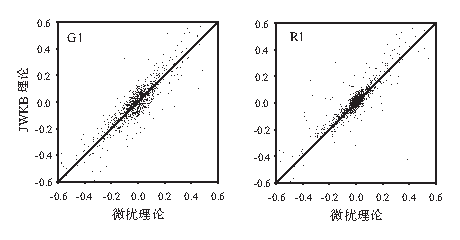
\includegraphics{../figures/chap16/fig16.eps}
}
\end{tabular}
&
\parbox{3.5cm}{\small
Figure~16.15. Schematic amplitude radiation pattern
$|R(\zeta_{\rm s})|$
of a typical surface wave.  A great-circle
ray on a spherically symmetric Earth leaves the source
at an azimuth $\zeta_{\rm s}$, whereas the corresponding
perturbed ray on a laterally heterogeneous leaves at
an azimuth $\zeta_{\rm s}+\delta\zeta_{\rm s}$.
}
\end{tabular}
\end{figure}
\addtocounter{figure}{1}
\begin{figure}[!b]
\begin{center}
\scalebox{1.1}{
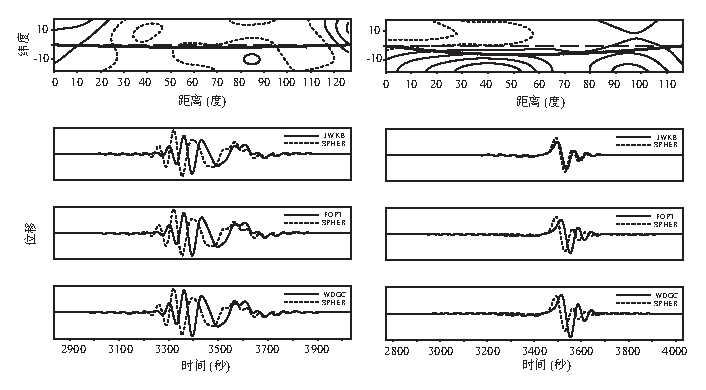
\includegraphics{../figures/chap16/fig17.eps}
}
\end{center}
\caption[amp]{\label{fig:16.amp}
Scatter-plot comparison of the first-order amplitude anomaly
$\delta A/A$ (due to both path and source effects) with the exact
JWKB anomaly $(A-A_{\rm spher\,\oplus})/A_{\rm spher\,\oplus}$ for
165-second fundamental-mode surface waves on model S12WM13.
Each of the 850 points represents a single G1 or R1 path.
The exact anomalies incorporate the geographical variations
in the eigenfunctions $U_{\rm s},V_{\rm s},W_{\rm s}$ and $U,V,W$ 
at the source and receiver, which have been neglected in the
perturbation analysis.}
\end{figure}

Figure~\ref{fig:16.amp} shows a comparison of the first-order
amplitude anomalies $\delta A/A=
\delta A_{\rm p}/A_{\rm p}+\delta A_{\rm s}/A_{\rm s}$
obtained using ray perturbation theory with the exact ray-theoretical
anomalies $(A-A_{\rm spher\,\oplus})/A_{\rm spher\,\oplus}$
for a number of G1 and R1 minor-arc paths on model S12WM13.
It is evident that $\delta A/A$ is more discrepant than the
first-order takeoff-angle and arrival-angle anomalies
$\delta\zeta_{\rm s}$ and $\delta\zeta$
exhibited in Figure~\ref{fig:16.takeoff},
and that these in turn are more discrepant than the
first-order Fermat phase anomalies $\delta\psi_{\rm p}$
in Figure~\ref{fig:16.phase}; this reflects the
respective dependence of the dominant contributions
to these quantities upon the second, first and zeroth
cross-path derivatives $\p_{\theta}^2\delta c$,
$\p_{\theta}\delta c$ and $\delta c$. 

\renewcommand{\thesubsection}{$\!\!\!\raise1.3ex\hbox{$\star$}\!\!$
\arabic{chapter}.\arabic{section}.\arabic{subsection}}
\subsection{Synthetic seismogram comparisons}
\index{seismogram!surface-wave|(}%
\index{surface-wave seismogram|(}%
\renewcommand{\thesubsection}{\arabic{chapter}.\arabic{section}.\arabic{subsection}}

Figure~\ref{fig:16.comparison} shows two examples
of surface-wave synthetic seismograms computed upon
Earth model S12WM13 using the methods described in
this chapter.  The left column shows the ray paths and
radial-component waveforms of R1 Rayleigh waves recorded at station
CTAO in Charters Towers, Australia, following the February 16, 1979
earthquake located near the coast of Peru,
\index{Peru 1979 earthquake}%
whereas the right column shows
the ray paths and transverse-component waveforms of G1 Love waves recorded
at station BJT in Beijing, China, following the November 29, 1978
Oaxaca, Mexico event.
\index{Oaxaca 1978 earthquake}%
The top panels show the exact ray deviations
from the unperturbed great-circle paths, superimposed upon a map of the
fractional phase-speed perturbation $\delta c/c$
for165-second G1 and R1 waves along a strip from source to receiver.
The bottom three panels compare three methods of computation:
(1) exact JWKB theory based
upon Runge-Kutta integration of the kinematic and dynamical
ray-tracing equations, with the geographical variations
in the radial eigenfunctions $U_{\rm s},V_{\rm s},W_{\rm s}$
and $U,V,W$ at the source and receiver fully accounted for;
(2) first-order ray perturbation theory, with the lateral
variations in $U_{\rm s},V_{\rm s},W_{\rm s}$ and $U,V,W$
ignored; (3) the Woodhouse-Dziewonski great-circle approximation,
which accounts for the lateral heterogeneity by means of a fictitious
frequency and source shift $\om\rightarrow\om+\delta\bar{\omega}$
and $\Theta\rightarrow\Theta+\delta\Theta$ in a spherical-Earth
normal-mode summation code.  The synthetic displacement seismograms
$\bnuh\cdot\bs(\bx,t)$ incorporate all fundamental-mode waves with periods
$T=2\pi/\om$ in the range 50--500 seconds; the group-speed windows are
3.2--4.7~km/s for the Love waves and 3.5--5.0~km/s for the Rayleigh
waves, respectively.  The corresponding spherical-Earth seismogram
is used as the standard of comparison in each panel.
The R1 ray path from Peru to CTAO is 
deflected by only about $2^\circ$ from the unperturbed
great circle; the JWKB waveform in this case is quite
well approximated by both first-order perturbation
theory and the great-circle approximation.
There is a slight discrepancy in amplitude;
however, the phases agree with each other
nicely throughout the waveform.
This particular ray path traverses a
low-speed region in the South Pacific,
so there is a marked phase delay
relative to the spherical Earth.
The G1 ray path from Oaxaca to Beijing
travels along the Pacific coastal region,
and is deflected by about $5^\circ$ from the unperturbed great circle. 
In this case, there is a significant discrepancy between the JWKB
waveform and the waveforms predicted by first-order perturbation theory
\begin{figure}[!t]
\begin{center}
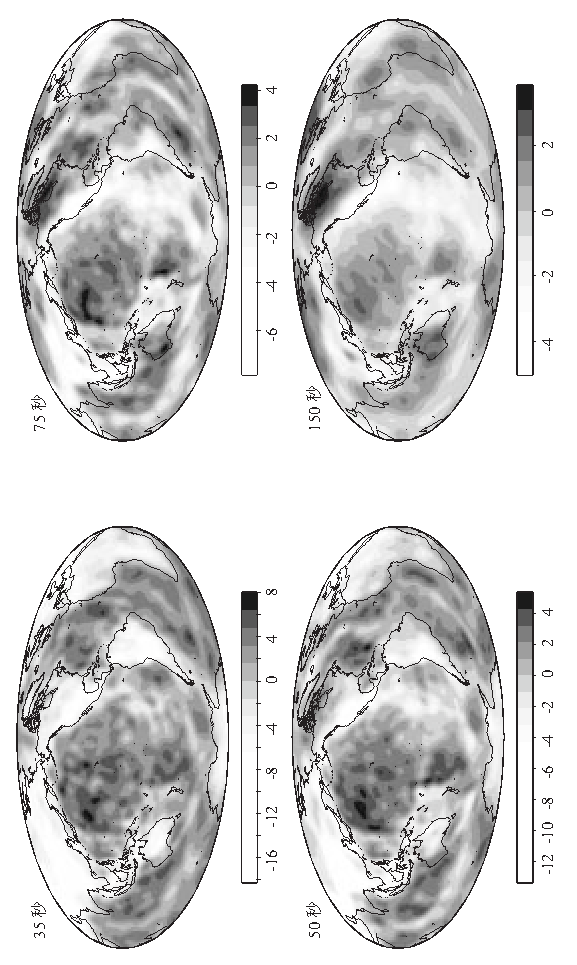
\includegraphics{../figures/chap16/fig18.eps}
\end{center}
\caption[comparison]{\label{fig:16.comparison}
({\em Top left\/}) JWKB ray path for R1 waves from the
February 16, 1979 Peru event to station CTAO in Charters Towers,
Australia, superimposed on a contour map of $\delta c/c$ for
165-second fundamental-mode Rayleigh waves on model S12WM13.
({\em Top right\/}) JWKB ray path for G1 waves from the November 11,
1978 Oaxaca event to station BJT in Beijing, China,
superimposed on a contour map of $\delta c/c$ for
165-second fundamental-mode Love waves on model S12WM13.
The maps have been rotated so that the source and receiver are
situated on the equator at the left and right, respectively;
this is the coordinate system used to trace surface-wave rays.
The JWKB and great-circle ray paths are indicated by the heavy
solid line and the long-dashed line, whereas positive and negative
values of $\delta c$ are indicated by the light solid contours and
the short-dashed contours, respectively; the contour interval is 1\%.
The remaining panels show the JWKB synthetic displacement seismograms
({\em second from top\/}), the corresponding seismograms computed using
first-order ray perturbation theory ({\em third from top\/}), and the
seismograms computed using the Woodhouse-Dziewonski great-circle
approximation ({\em bottom\/}).  Full scale on the radial-component
R1 seismograms ({\em left\/}) is 0.28~mm, whereas that on the
transverse-component G1 seismograms ({\em right\/}) is 4.06~mm.
The waveforms on
model S12WM13 ({\em solid lines\/}) are in each case compared with
the fundamental-mode spherical-Earth seismograms ({\em dashed lines\/}).
The label SPHER designates the spherical-Earth synthetic,
FOPT is an acronym for first-order ray-perturbation theory,
and WDGC is an acronym for the Woodhouse-Dziewonski great-circle
approximation. A 10\% cosine taper has been applied to both ends of
the spectrum in the frequency domain in order to suppress ringing
in the time series.}
\end{figure}
and the great-circle approximation.  The Oaxaca to Beijing path is
transitional in character, with a large cross-path gradient
$\p_{\theta}\delta c$.  In general, the two approximations
perform poorly for such ray paths; they perform best for locally
fast or slow paths that tend to cross contours of $\delta c$
\index{seismogram!surface-wave|)}%
\index{surface-wave seismogram|)}%
\index{ray perturbation theory!surface waves|)}%
\index{surface-wave perturbation theory|)}%
\index{perturbation!surface waves|)}%
at relatively steep angles, rather than run along them.

\section{Surface-Wave Tomography}
\index{surface-wave tomography|(}%
\index{tomography!surface-wave|(}%
\label{16.sec.eqrot}

Our emphasis in this chapter has been upon the development
of JWKB methods for solving the {\em forward problem\/} of
\index{forward problem}%
synthesizing synthetic long-period surface-wave seismograms
upon a smooth, laterally heterogeneous Earth.  In this final
section, we describe a number of approaches that have been
used to address the surface-wave {\em inverse problem\/}:
\index{inverse problem}%
\begin{quote}
Given a suite of observed waveforms $\ba_{\rm obs}(\bx,t)$
excited by earthquakes with known origin times $t_{\rm s}$,
hypocentral locations $\bx_{\rm s}$ and moment tensors $\bM$,
find the three-dimensional perturbations
$\delta\hspace{-0.1 mm}\kappa$, $\delta\hspace{-0.2 mm}\mu$,
$\delta\hspace{-0.2 mm}\rho$, $\delta\hspace{-0.1 mm}d$
or $\delta\hspace{-0.1 mm}\alpha$,
$\delta\hspace{-0.2 mm}\beta$, $\delta\hspace{-0.1 mm}\rho$,
$\delta\hspace{-0.1 mm}d$ to the known average
spherically symmetrical structure of the Earth.
\end{quote}
Our emphasis is upon the assumptions and approximations
that underlie the inversion procedures; we refrain from
presenting or comparing any results, inasmuch as these are
more fruitfully discussed within the broader context of global
seismic tomography and geodynamics---topics that are beyond
the scope of this book.

\subsection{Woodhouse-Dziewonski method}
\index{Woodhouse-Dziewonski method|(}%

The modern era of three-dimensional mantle structural
studies was inaugurated by Woodhouse \& Dziewonski
(\citeyear{woodhouse&dziewonski84}), as we noted
in Chapter~1.  This pioneering investigation developed
a method of {\em waveform fitting\/}, based
\index{waveform fitting}%
upon the {\em great-circle approximation\/} discussed
\index{great-circle approximation}%
\index{path-average approximation}%
in Section~\ref{16.sec.WDGC}, that is still in use today.
A long-period accelerogram $a(t)=\bnuh\cdot\ba(\bx,t)$
is written as a sum over
normal-mode multiplets ${}_n{\rm S}_l$ and ${}_n{\rm T}_l$
of the form~(\ref{10.appacc}):
\eq \label{16.WDGC1}
a(t)=\sum_{\rm multiplets}\hspace{-3.0 mm}A\cos\om t\exp(-\gamma t).
\en
Elastic lateral heterogeneity is taken into account by means
of a fictitious frequency shift $\delta\bar{\omega}$ and source
shift $\delta\Theta$.  The resulting perturbation to
the accelerogram~(\ref{16.WDGC1}) is
\eq \label{16.WDGC2}
\delta a(t)=\sum_{\rm multiplets}\hspace{-3.0 mm}[\delta\Theta\,
\p_{\Theta}A\cos\om t-\delta\bar{\omega}\,A\sin\om t]
\exp(-\gamma t).
\en
The partial derivative $\p_{\Theta}A$ may be
readily evaluated by making use of
equations~(\ref{10.vectamp})--(\ref{10.Dexpl2}).
Upon making use of~(\ref{16.WD4}) we can rewrite~(\ref{16.WDGC2})
in terms of the minor-arc plus the great-circular average
of the local eigenfrequency perturbation:
\eqa \label{16.WDGC3} \lefteqn{
\delta a(t)=\sum_{\rm multiplets}\hspace{-3.0 mm}
\delta\hat{\omega}\,(c/C\hspace{0.3 mm}\om)
\p_{\Theta}A\cos\om t\exp(-\gamma t)} \nonumber \\
&&\mbox{}-\sum_{\rm multiplets}\hspace{-3.0 mm}
\delta\bar{\omega}\,[A\sin\om t+(c/C\hspace{0.3 mm}\om)
\p_{\Theta}A\cos\om t]\exp(-\gamma t).
\ena
The perturbation $\delta\om(\theta,\phi)$ is identical
to that of a spherical Earth having the same structure
as that underlying the point $a,\theta,\phi$.  For brevity
in what follows, we abbreviate the dependence~(\ref{eq:9.delomiso})
upon $\delta\hspace{-0.1 mm}\kappa$, $\delta\hspace{-0.2 mm}\mu$,
$\delta\hspace{-0.2 mm}\rho$, $\delta\hspace{-0.1 mm}d$
or~(\ref{eq:9.delomiso2}) upon $\delta\hspace{-0.1 mm}\alpha$,
$\delta\hspace{-0.2 mm}\beta$, $\delta\hspace{-0.1 mm}\rho$,
$\delta\hspace{-0.1 mm}d$ using the symbolic notation
\eq \label{16.WDGC4}
\delta\om=\int_0^a\delta\earth\,K_{\subearth}\,dr.
\en
Upon expanding the structural perturbations in terms
of real surface spherical harmonics,
\eq \label{16.WDGC5}
\delta\earth=\sum_{st}\delta\earth_{st}\sY_{st},
\en
we may express the unknown quantities in~(\ref{16.WDGC3}) in the form
\eq \label{16.WDGC6}
\delta\hat{\omega}=\sum_{st}\left[\int_0^a
\delta\earth_{st}\,K_{\subearth}\,dr\right]\hat{\sY}_{st},
\en
\eq \label{16.WDGC7}
\delta\bar{\omega}=\sum_{st}\left[\int_0^a
\delta\earth_{st}\,K_{\subearth}\,dr\right]\bar{\sY}_{st}.
\en
The minor-arc and great-circular averages $\hat{\sY}_{st}$
and $\bar{\sY}_{st}$ of $\sY_{st}$ are known functions,
which may be readily calculated by rotation of the
source-receiver path to the equator, as discussed in
Appendices~\ref{section:B.9} and~\ref{section:C.8.7}.
Upon substituting~(\ref{16.WDGC6})--(\ref{16.WDGC7})
we obtain a linearized relation between the perturbation
$\delta a(t)$ and the coefficients $\delta\earth_{st}(r)$
describing a three-dimensional Earth model:
\eq \label{16.WDGC8}
\delta a(t)=\sum_{st}\int_0^a\delta\earth_{st}(r)
\,K_{\subearth st}(r,t)\,dr,
\en
where
\eqa \label{16.WDGC9} \lefteqn{
K_{\subearth st}=\sum_{\rm multiplets}\hspace{-3.0 mm}(c/C\hspace{0.2 mm}\om)
\p_{\Theta}A\cos\om t\exp(-\gamma t)
\,K_{\subearth}\,\hat{\sY}_{st}} \\
&&\mbox{}-\sum_{\rm multiplets}
\hspace{-3.0 mm}[A\sin\omega t
+(c/C\hspace{0.2 mm}\om)
\p_{\Theta}A\cos\om t]\exp(-\gamma t)
\,K_{\subearth}\,\bar{\sY}_{st}. \nonumber
\ena
Equations~(\ref{16.WDGC8})--(\ref{16.WDGC9})
provide the basis for an iterative least-squares
inversion, which seeks to minimize the
residual $\sum_{\rm paths}\int_{t_1}^{t_2}
[a(t)-a_{\rm obs}(t)]^2\,dt$
between a suite of synthetic and observed seismograms;
the fictitious frequency and source location are updated,
$\om\rightarrow\om+\delta\bar{\om}$, $\Theta\rightarrow
\Theta+\delta\Theta$, and the kernels $K_{\subearth st}(r,t)$
are computed anew at each iteration.  The principal advantage
of the procedure is that it enables the entire long-period
waveform $a_{\rm obs}(t)$ to be used as a constraint upon the unknown
parameters $\delta\earth_{st}$; in particular, all of the higher-overtone
($n=1,2,\ldots$) modes which propagate with very nearly the same group speed
are included in addition to the multi-orbit,
fundamental-mode ($n=0$) surface waves.
\index{Woodhouse-Dziewonski method|)}%

\subsection{Partitioned-waveform method}
\index{partitioned-waveform method|(}%

In regions with many peripheral sources and stations,
giving rise to good crossing-path coverage, it is
possible to obtain higher-resolution models of
crustal and upper-mantle structure by
incorporating higher-frequency body and surface waves.
The so-called {\em partitioned-waveform method\/}
was developed by Nolet~(\citeyear{nolet90}),
expressly for use in such applications.
In this approach, attention is restricted
to the minor-arc ($s=1$) arrivals in~(\ref{16.accsum}).
Fermat's principle is invoked to calculate the path
contribution to the phase, and amplitude variations
due to ray-tube focusing and defocusing are ignored;
the frequency-domain acceleration response $a(\om)$
is written as a sum over surface-wave modes or dispersion
branches of the form
\eqa \label{16.Nolet1}
\lefteqn{
a(\om)=\sum_{\rm modes}A_{\rm r}\exp (-i\psi_{\rm r})
A_{\rm s}\exp (-i\psi_{\rm s})(8\pi k\sin\Theta)^{-1/2}}  \nonumber\\
&&\mbox{}
\times\exp (-ik\Theta)\exp(-i\,\delta\hat{k}\,\Theta)
\exp(-\om\Theta/2CQ),
\ena
where $k$, $C$ and $Q^{-1}$ are the unperturbed spherical-Earth
wavenumber, group speed and reciprocal quality factor, and
the known source and receiver contributions
$A_{\rm s}\exp(-i\psi_{\rm s})$ and $A_{\rm r}\exp(-i\psi_{\rm r})$
are given by equations~(\ref{16.dAs}) and~(\ref{16.dAr}).
The only unknown in the JWKB-Fermat representation~(\ref{16.Nolet1})
is the minor-arc average
\eq
\delta\hat{k}=\frac{1}{\Theta}\int_0^\Theta\delta k
\,d\Delta
\en
of the local wavenumber perturbation
$\delta k$.  It can be expressed in terms of the
corresponding average
\eq \label{16.Nolet2}
\delta\hat{\earth}
=\frac{1}{\Theta}\int_0^\Theta\delta\earth
\,d\Delta
\en
of the three-dimensional structure
along the unperturbed great-circular
ray path in the symbolic form
\eq \label{16.Nolet3}
\delta\hat{k}=-C^{-1}\int_0^a
\delta\hat{\earth}\,K_{\subearth}\,dr.
\en
In the first step, the time-domain misfit
$\int_{t_1}^{t_2}[a(t)-a_{\rm obs}(t)]^2\,dt$
of a suitably windowed portion of every seismogram
is minimized using a nonlinear optimization procedure
to find the best-fitting {\em path-average perturbation\/}
\index{path-average perturbation}%
$\delta\hat{\earth}(r)$.  Since the dimension of the
radially parameterized model space is relatively
small, it is possible to conduct a robust and efficient
nonlinear search using the conjugate gradient algorithm.
Local minima can be avoided by filtering $a_{\rm obs}(t)$,
and fitting the long-period portion of the waveform first.
In the second step, the averages along
a collection of paths are combined to
determine the three-dimensional structure
$\delta\earth(r,\theta,\phi)$ in the region.
Every seismogram provides a separate {\em linear\/}
constraint via the relation~(\ref{16.Nolet2}).
Diagonalization of the Hessian matrix of second
partial derivatives of the misfit function
yields a system of {\em independent\/} linear
equations with known variances on the right side,
enabling a resolution analysis to be performed.
A major advantage of the partitioned-waveform
method is its great flexibility.  Different
elastic and anelastic background models
$\earth$, $Q^{-1}$ may be used along
different paths, and different eigenfunctions
$U_{\rm s}$, $V_{\rm s}$, $W_{\rm s}$ and $U,V,W$
may be used at every source and receiver, if it is
appropriate.  Higher overtones ($n=1,2,\ldots$)
are included in the JWKB-Fermat sum~(\ref{16.Nolet1}),
just as they are included in the Woodhouse-Dziewonski
great-circle approximation~(\ref{16.WDGC1}),
so that triplicated S waves in the epicentral
distance range $0^\circ\leq\Theta\leq 30^\circ$
and SS, SSS,\hspace{0.2mm}$\ldots$ multiples can be
incorporated in the fitting procedure as well
as fundamental-mode G1 and R1 waves.
The method has been used by Nolet and his co-workers
to obtain high-quality images of the upper-mantle
shear-wave speed $\delta\hspace{-0.2 mm}\beta$
beneath central Europe (Zielhuis \& Nolet
\citeyear{zielhuis&nolet94}), North
America (Van der Lee \citeyear{vanderlee96};
Van der Lee \& Nolet \citeyear{vanderlee&nolet97})
and the Philippine Sea plate
(Lebedev, Nolet \& Van der Hilst
\citeyear{lebedev&al97}).
\index{partitioned-waveform method|)}%

\subsection{Phase-speed tomography}
\index{phase-speed tomography|(}%
\index{tomography!phase-speed|(}%
\index{single-station method|(}%

Rather than fitting a single three-dimensional Earth model
$\delta\earth$ or a suite of separate path-average models
$\delta\hat{\earth}$ to a suite of observed frequency-domain
seismograms
\eq \label{16.whoop1}
a_{\rm obs}(t)=\sum_{\rm modes}\sum_{\rm rays}
A_{\rm obs}\exp(-i\psi_{\rm obs}),
\en
many workers prefer
to extract the amplitudes $A_{\rm obs}$ and phases
$\psi_{\rm obs}$ of the constituent surface waves.
Indeed, this is the classical approach to surface-wave
tomography, as we noted in Chapter~1.  The method is
most easily applied to the long-period fundamental-mode
waves, since they are relatively well isolated from the
earlier-arriving overtones.  The strong dispersion
over long source-receiver paths gives rise to a rapid
variation of phase $\psi_{\rm obs}$ with frequency
$\omega$; a straightforward Fourier or periodogram
analysis is known to yield a biased spectral estimate
in such circumstances.  To reduce this bias, it is
necessary to ``de-disperse'' the waveform; this is
commonly done using a cross-spectral or matched-filter
\index{matched filter}%
technique, which measures the residual amplitude
$\delta A=A_{\rm obs}-A_{\rm spher\,\oplus}$
and phase $\delta\psi=\psi_{\rm obs}-\psi_{\rm spher\,\oplus}$
relative to those of a spherical-Earth synthetic seismogram
\eq \label{16.whoop2}
a_{\rm spher\,\oplus}(t)=\sum_{\rm modes}\sum_{\rm rays}
A_{\rm spher\,\oplus}\exp(-i\psi_{\rm spher\,\oplus}).
\en
The source contribution $\delta\psi_{\rm s}$ to the
phase difference is generally ignored; in that case,
$\delta\psi=\delta\psi_{\rm p}$ can be related
to the surface-wave phase-speed perturbation $\delta c$
either by the first-order Fermat approximation
\eq \label{16.whoop3}
\delta\psi=-\om c^{-2}\underbrace{\int_{\hat{\mbox{\bf\scriptsize r}}_{\rm s}}
^{\hat{\mbox{\bf\scriptsize r}}}\delta c\,d\Delta}_{\rm great\;circle}
\en
or the exact JWKB relation
\eq \label{16.whoop4}
\delta\psi=\om\underbrace{\int_{\hat{\mbox{\bf\scriptsize r}}_{\rm s}}
^{\hat{\mbox{\bf\scriptsize r}}}\frac{d\Delta}{c+\delta c}}_{\rm true\;ray\;path}
-\frac{\om\Delta}{c}.
\en
Equations~(\ref{16.whoop3}) and~(\ref{16.whoop4})
provide the foundation for phase-speed tomography;
the perturbation $\delta c$ may be either expanded in
surface spherical harmonics $\sY_{st}$ (Wong \citeyear{wong89})
or parameterized in terms of local basis functions using a block
or triangular tesselation of the unit sphere (Zhang \& Tanimoto
\citeyear{zhang&tanimoto93}; Wang, Tromp \& Ekstr\"{o}m
\citeyear{wang&al98}).  In practice, most tomographic
analyses do not go beyond the Fermat approximation~(\ref{16.whoop3}).
If the geographical variations in $\delta c$ are pronounced,
an initial Fermat
model may be iteratively refined by tracing rays through
$c+\delta c$ and making use of~(\ref{16.whoop4}).
Independent phase-delay measurements $\delta\psi$
can be collected not only for $s=1$ minor-arc paths,
but also for $s=2,3,\ldots$ multi-orbit arrivals.
Great-circle phase delays $\delta\psi_{s+2}
-\delta\psi_s$ can also be measured by analysis
of circumnavigational waves; these data
have the added advantage that they are independent of the
moment tensor $\bM$.  At periods $T=2\pi/\om$ less
than 100--150~seconds, the lateral perturbations in
phase speed $\delta c$ are large enough to cause path
variations~(\ref{16.whoop3})--(\ref{16.whoop4})
of several cycles in phase; an isolated measurement
of the phase anomaly $\delta\psi$ at a single period is in this
case indistinguishable from $\delta\psi\pm 2N\pi$.
This so-called {\em cycle-skip\/} ambiguity can
\index{cycle skip}%
be eliminated by means of a ``bootstrap''
technique, in which the correct $(N=0)$
cycle count is anchored at longer periods,
where it is almost always the case that
$|\psi_{\rm obs}-\psi_{\rm PREM}|\leq\pi$;
the measurements can subsequently be extended to
shorter periods by requiring that the observed
dispersion relation be continuous.
Uncertainties can be assigned to measurements of
$\delta\psi$ in a straightforward manner;
the resulting geographical maps of $\delta c$ can be regarded
as intermediate ``observables'', which can be compared
and utilized in conjunction with other
data to constrain the three-dimensional
elastic structure of the Earth $\delta\earth$.

Modern surface-wave phase-speed studies
are able to exploit the large and ever-growing
data set of broad-band digital recordings
from several global and regional seismographic
networks.  Table~16.1 compares the characteristics
of some recent tomographic analyses; the total number of
source-receiver paths for which the phase difference
$\delta\psi$ has been measured is truly impressive!
The study by Laske \& Masters (\citeyear{laske&masters96})
is unique in that it incorporates surface-wave arrival-angle
measurements $\delta\zeta$ obtained by means of a multi-taper
polarization analysis of three-component recordings, as well
as phase measurements $\delta\psi$.  The first-order
relation~(\ref{16.arrival2}) was used to fit
the arrival-angle data; the dependence of $\delta\zeta$
upon the cross-path derivative of $\delta c$ enhances the
resolution of high-degree structure.  As an unexpected
by-product of their analysis, Laske \& Masters detected
$5^{\circ}\!-\!15^{\circ}$ misalignments of the
``north-south'' and ``east-west'' components at
several stations of the Global Seismographic Network!
\begin{table}[!b]
\centering
\begin{tabular}{|l|c|c|} \hline
&& \\
\hspace{15.0 mm}Reference &  Period Range & Number of Paths \\
&& \\ \hline
&& \\
Trampert \& Woodhouse (\citeyear{trampert&woodhouse95})
& 40--150 s & 24,000 \\
Trampert \& Woodhouse (\citeyear{trampert&woodhouse96})
& 40--150 s & 62,000 \\
Zhang \& Lay (\citeyear{zhang&lay96})
& 85--250 s & 30,000 \\
Ekstr\"{o}m, Tromp \& Larson (\citeyear{ekstrom&al96})
& 35--150 s & 56,000 \\
Laske \& Masters (\citeyear{laske&masters96})
& 75--250 s & 11,000 \\
&& \\ \hline
\end{tabular}
\caption[lotsa paths]{Period range and number of source-receiver
paths incorporated in some recent fundamental-mode Love and Rayleigh
phase-speed analyses.}
\end{table}

Figures~\ref{fig:16.phase_mapsL} and~\ref{fig:16.phase_mapsR}
illustrate the relative variations $\delta c/c$
in Love and Rayleigh phase speed obtained by
Ekstr\"{o}m, Tromp \& Larson (\citeyear{ekstrom&al96}).
These $s_{\rm max}=40$ models explain $70\!-\!96$\%
of the variance in the observed phase residuals
$\psi_{\rm obs}-\psi_{\rm PREM}$, testifying to
the high quality and internal consistency of the
original dispersion measurements.  Many of the most
prominent features in these maps---such as the slow wave
speeds in the vicinity of the Iceland hotspot and Red Sea
rift zone---are seen in other studies as well, and have
an obvious tectonic explanation or interpretation.  At longer
periods ($2\pi/\om>150$~s for Love waves and $2\pi/\om>75$~s
for Rayleigh waves) the stable continental cratons exhibit fast
speeds, whereas the mid-oceanic ridges are comparatively slow.
The expected increase in wave speed in the older and deeper
ocean basins, due to the cooling of the spreading lithosphere,
is also apparent.
\begin{sidewaysfigure}
\begin{center}
\rotatebox{270}
{
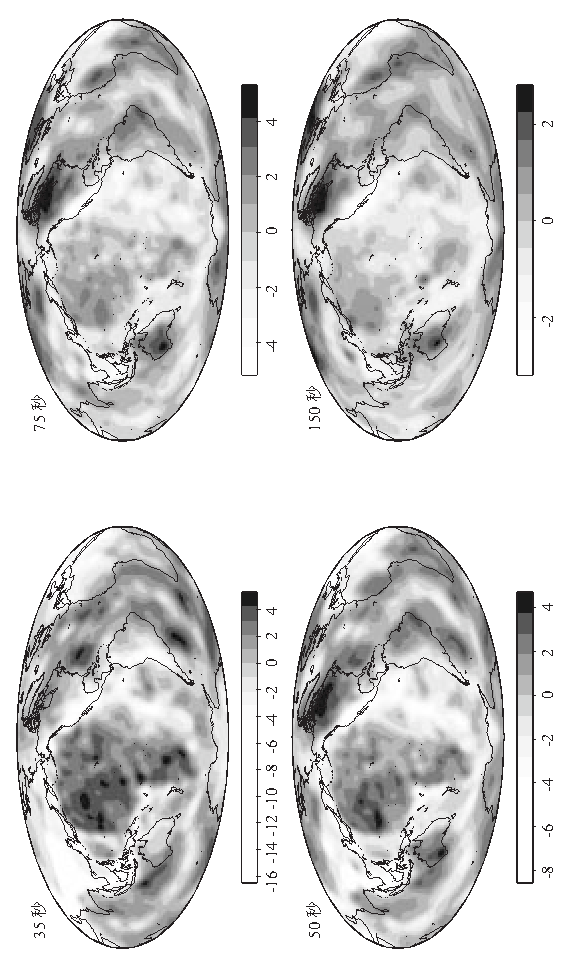
\includegraphics{../figures/chap16/fig19.eps}
}
\end{center}
\caption[phase_mapsL]{
Global Love-wave phase-speed maps $\delta c/c$
(in percent) at periods of 35, 50, 75 and 150~seconds.
Notice that the grey scales differ from map to map.
}
\label{fig:16.phase_mapsL}
\end{sidewaysfigure}
\begin{sidewaysfigure}
\begin{center}
\rotatebox{270}
{
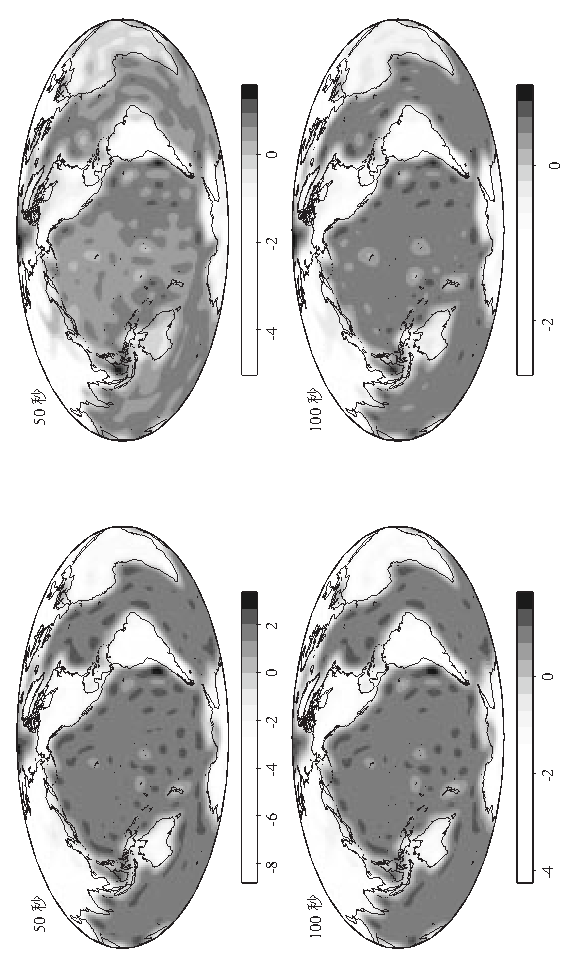
\includegraphics{../figures/chap16/fig20.eps}
}
\end{center}
\caption[phase_mapsR]{
Global Rayleigh-wave phase-speed maps $\delta c/c$
(in percent) at periods of 35, 50, 75 and 150~s.
Notice that the grey scales differ from map to map.
}
\label{fig:16.phase_mapsR}
\end{sidewaysfigure}
\begin{sidewaysfigure}
\begin{center}
\rotatebox{270}
{
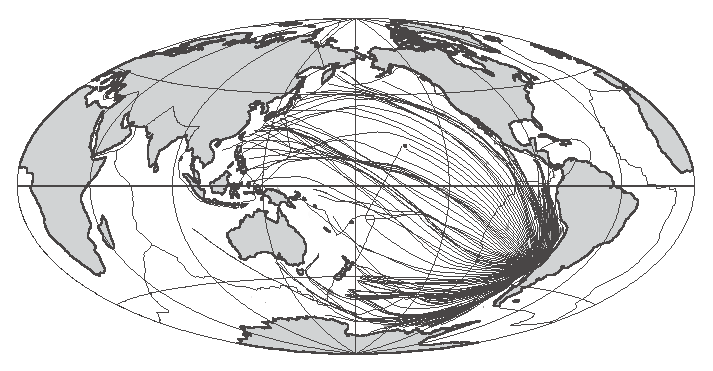
\includegraphics{../figures/chap16/fig07.eps}
}
\end{center}
\caption[crustal]{
Relative perturbation $\delta c/c$ in the phase speed
of fundamental-mode Love waves ({\em left\/}) and
Rayleigh waves ({\em right\/}) due to lateral variations
in the thickness and structure of the Earth's crust.
The perturbations are shown at two periods: 50~s
({\em top\/}) and 100~s ({\em bottom\/}). Note that
the grey scales differ from map to map.
}
\label{fig:16.crustal}
\end{sidewaysfigure}

Prior to utilizing maps such as those in Figures~\ref{fig:16.phase_mapsL}
and~\ref{fig:16.phase_mapsR} as constraints upon the three-dimensional
structure $\delta\hspace{-0.1 mm}\alpha$, $\delta\hspace{-0.2 mm}\beta$,
$\delta\hspace{-0.2 mm}\rho$, $\delta\hspace{-0.1 mm}d$ of the upper
mantle, it is necessary to correct for the effect of lateral variations
\index{crustal correction}%
in the thickness and structure of the crust.  First-order perturbation
theory may not provide an adequate correction at short and intermediate
periods; to illustrate this, we account for crustal variations by stripping
the spherically symmetric crust from PREM and replacing it with the laterally
variable model CRUST~5.1 (Mooney, Laske \& Masters \citeyear{mooney&al98}).
Subsequently, at selected angular frequencies, we calculate the exact local
modes on a grid of points $\theta,\phi$ and fit surface spherical harmonics
$\sY_{st}$ to the associated distribution of local surface-wave phase speed
$\delta c_{\rm crust}$.  The resulting crustal phase-speed anomalies are
depicted in Figure~\ref{fig:16.crustal}. In active compressional orogens,
such as the Alpine-Himalayan belt and the Tibetan Plateau, where the
crustal thickness exceeds 70~km, the phase-speed correction for 50~s
Love waves is $-12\%\leq\delta c_{\rm crust}\leq-10\%$. 
In fact, the phase speed of these short-period waves is dominated by
the effects of crustal structure; the Fr\'{e}chet kernel
$K_{\beta}$ for 50~s Love waves
is negligible below a depth of 50--60~km, so it is no surprise that
the observed and predicted maps in
Figures~\ref{fig:16.phase_mapsL} and~\ref{fig:16.crustal} look almost the same.
At periods greater than 150~s the crustal correction is much less significant,
particularly for Rayleigh waves.

The phase residuals $\psi_{\rm obs}-\psi_{\rm PREM}$
of higher-mode Love and Rayleigh waves are much more difficult
to measure reliably, because of the near coincidence of the
$2\pi/\omega\leq 50\!-\!100$~s group arrivals in the time domain
(see Sections~11.6.1--11.6.2 and~11.7.1).  The pioneering analyses of
Nolet (\citeyear{nolet77}) and Cara (\citeyear{cara78}), which
we discussed in the introduction, employed multi-station array
methods to disentangle the $n=1,2,\ldots$ overtone branches. In a subsequent
study, Stutzmann \& Montagner (\citeyear{stutzmann&montagner93};
\citeyear{stutzmann&montagner94}) made use of a single-station
method which exploits recordings from a number of closely
spaced earthquake sources.  This technique is most effective when
the sources have significantly different focal depths, so
that the excitation amplitudes of the target branches
are very different; unfortunately, the number of paths having
the requisite multi-source geometry is limited, leading to poor
lateral resolution of the phase-speed perturbations $\delta c$.
The development of single-station, single-source methods based
upon cross-correlation with single-branch spherical-Earth
seismograms would obviously be desirable; Van Heijst \& Woodhouse
(\citeyear{vanheijst&woodhouse97}) have made some recent
\index{phase-speed tomography|)}%
\index{tomography!phase-speed|)}%
\index{single-station method|)}%
progress toward this daunting goal.

\subsection{Anelastic tomography}
\index{anelastic tomography|(}%
\index{tomography!anelastic|(}%

A number of investigators have attempted to use
measured G1, G2,\hspace{0.2mm}$\ldots$ and R1, R2,\hspace{0.2mm}$\ldots$
amplitude anomalies $\delta A=A_{\rm obs}-A_{\rm PREM}$
to constrain global lateral variations in the anelasticity
$\delta Q^{-1}/Q^{-1}$ of the Earth.  This has proven
to be an extremely intractable problem, because of the
large number of additional effects which can give rise
to comparable surface-wave amplitude variations,
including uncertainties in the locations $\bx_{\rm s}$
and mechanisms $\bM$ of earthquake sources,
as well as ray-tube focusing and defocusing,
and other influences of the imperfectly known
elastic lateral heterogeneity $\delta c$,
such as the radiation-pattern effect
illustrated in Figure~16.15.
The total fractional amplitude perturbation
is given by
\eq \label{16.intrinsic}
\frac{\delta A}{A}=
\frac{\delta A_{\rm g}}{A_{\rm g}}
+\;\exp\left(-\frac{\omega}{2CQ}\int_0^{\Delta}
\frac{\delta Q^{-1}}{Q^{-1}}\,d\Delta\right)-1,
\en
where the term $\delta A_{\rm g}/\hspace{-0.4 mm}A_{\rm g}
=\delta A_{\rm p}/\hspace{-0.4 mm}A_{\rm p}
+\delta A_{\rm s}/\hspace{-0.4 mm}A_{\rm s}
+\cdots$ encapsulates the competing geometric
path, source and other effects, and the integral
is over the unperturbed great-circular ray path
of a minor-arc or higher-orbit wave.
Several approaches have been used
to deal with the geometrical variations
in global anelastic tomographic studies.
It is not feasible simply to correct for
the effects of lateral wave-speed variations
$\delta c$ using existing phase-speed maps,
because of the strong dependence
of $\delta A_{\rm p}/\hspace{-0.4 mm}A_{\rm p}$
upon short-wavelength structure, which is very
poorly constrained.  Early efforts sought to
exploit the observation that, in first-order
ray perturbation theory,
\eq \label{16.4data1}
\left(\frac{\delta A_{\rm p}}{A_{\rm p}}\right)_{s=4}-
\left(\frac{\delta A_{\rm p}}{A_{\rm p}}\right)_{s=2}+
\left(\frac{\delta A_{\rm p}}{A_{\rm p}}\right)_{s=3}-
\left(\frac{\delta A_{\rm p}}{A_{\rm p}}\right)_{s=1}=0,
\en
by virtue of the alternating odd and even
dependence~(\ref{16.relative2}) upon orbit
number $s$.  The source term
satisfies an analogous relation,
\eq \label{16.4data1p}
\left(\frac{\delta A_{\rm s}}{A_{\rm s}}\right)_{s=4}-
\left(\frac{\delta A_{\rm s}}{A_{\rm s}}\right)_{s=2}+
\left(\frac{\delta A_{\rm s}}{A_{\rm s}}\right)_{s=3}-
\left(\frac{\delta A_{\rm s}}{A_{\rm s}}\right)_{s=1}=0,
\en
because of the alternating
dependence~(\ref{16.takeoff2}) of the takeoff-angle
perturbation $\delta\zeta_{\rm s}$.
The composite four-orbit datum
\eq \label{16.4data2}
D=\frac{a_{s=4}}{a_{s=2}}\times
\frac{a_{s=3}}{a_{s=1}}
\en
should in this approximation depend only upon the
great-circular average of the anelastic perturbation:
\eq \label{16.4data3}
\delta D=\exp\left(-\frac{\omega}{CQ}\oint
\frac{\delta Q^{-1}}{Q^{-1}}\,d\Delta\right).
\en
Romanowicz (\citeyear{romanowicz90}) made use of
equation~(\ref{16.4data3}) to obtain the first
degree-two global model of upper-mantle anelasticity.
Synthetic studies by Durek, Ritzwoller \& Woodhouse
(\citeyear{durek&al93}) subsequently demonstrated that
departures from first-order ray perturbation theory
are sufficient to vitiate the linearized
relations~(\ref{16.4data1})--(\ref{16.4data1p})
as the sole basis of quantitative anelastic tomography.
They consider the quantity $D$ to be ``de-sensitized''
to phase-speed variations.  Prior to inverting for an
$s=2,4,6$ model of $\delta Q^{-1}$ they applied an additional
``de-biasing'' correction, based upon an existing map of
$\delta c$.  Romanowicz (\citeyear{romanowicz95}) used
single-orbit R1 and R2 amplitude measurements to obtain
the first global model of $\delta Q^{-1}$ with odd as
well as even degrees ($s=1\!-\!6$).
She sought to minimize the importance of
$\delta\hspace{-0.2 mm}A_{\rm s}/\hspace{-0.4 mm}A_{\rm s}$
and $\delta A_{\rm p}/\hspace{-0.4 mm}A_{\rm p}$
by heavy winnowing of the dataset, to eliminate
low-amplitude nearly nodal recordings and
measurements thought to have been strongly
affected by focusing and defocusing,
based upon a subjective criterion.
\index{anelastic tomography|)}%
\index{tomography!anelastic|)}%

\subsection{Beyond the path-average approximation}

All waveform inversion schemes based upon the JWKB approximation
share a common feature: the $s=1$ portion of a seismogram
$a(t)$ depends only upon the minor-arc path average
$\hat{\oplus}$ of the laterally heterogeneous elastic
structure $\earth$.  A change in the waveform
is related to a change in the Earth model via a {\em one-dimensional\/}
\index{Fr\'{e}chet kernel!one-dimensional}%
(radial) Fr\'{e}chet kernel:
\eq \label{16.LAST1}
\delta a=\int_0^a\delta\hat{\oplus}\,K_{\subearth}^{\rm 1D}\,dr.
\en
This is not an unreasonable approximation
for the fundamental-mode Love and Rayleigh waves,
but it is questionable for the earlier-arriving overtones.
Intuitively, one expects the sensitivity
of the early portion of a transverse-component
waveform $a(t)=\bPhih\cdot\ba(\bx,t)$
to be concentrated along the
associated SS, ${\rm SS}_{\rm SH}$,
${\rm SSS}_{\rm SH},\ldots$ body-wave rays.  Li \& Tanimoto
(\citeyear{li&tanimoto93}) demonstrated that the dependence
upon $\hat{\oplus}$ is fundamentally a consequence of the
absence of $n'\not=n$ cross-branch coupling in the JWKB
approximation.  By accounting for coupling between
${}_n{\rm T}_l$ and ${}_n{\rm S}_l$ multiplets
using a normal-mode representation of $a(t)$,
they obtained a {\em two-dimensional\/}
\index{Fr\'{e}chet kernel!two-dimensional}%
Fr\'{e}chet-kernel relationship of the form
\eq \label{16.LAST2}
\delta a=\int_{\Sigma}\delta\earth\,K_{\subearth}^{\rm 2D}\,dA,
\en
where $\Sigma$ denotes the unperturbed ray plane.
Equation~(\ref{16.LAST2}) has been used as the basis
of a global tomographic study by Li \& Romanowicz
(\citeyear{li&romanowicz95}; \citeyear{li&romanowicz96}).
Marquering \& Snieder (\citeyear{marquering&snieder95};
\citeyear{marquering&snieder96}) have developed a similar
two-dimensional ray-plane sensitivity relationship using
a more economical travelling-wave representation that accounts
for coupling between $n'\not= n$ dispersion branches.
Zhao \& Jordan (\citeyear{zhao&jordan97})
have used~(\ref{16.LAST2}) to develop
two-dimensional Fr\'{e}chet kernels for functionals
obtained by processing $a_{\rm obs}(t)$, such as travel-time anomalies
measured by cross-correlation with a spherical-Earth synthetic seismogram
$a_{\rm spher\,\oplus}(t)$.  
All of these investigations make use of
a stationary-phase approximation
which is valid only under the strong assumption that
the lateral variations in the direction perpendicular to the ray plane
are smooth.  To overcome this objection, Marquering, Nolet
\& Dahlen (\citeyear{marquering&al97}) have used the Born
approximation together with a travelling-wave representation
of $a(t)$ to obtain a fully three-dimensional waveform
sensitivity-kernel relationship of the form
\eq \label{16.LAST3}
\delta a=\int_{\subearth}\delta\earth\,K_{\subearth}^{\rm 3D}\,dV.
\en
These efforts to develop waveform and travel-time sensitivity
kernels which go beyond the one-dimensional path-average approximation
represent the current theoretical frontier in global seismic
tomography.  The subject is still in an active state of
development, and it is premature to attempt to provide
even a superficial synthesis at the present time.
\index{surface-wave tomography|)}%
\index{tomography!surface-wave|)}%
